%%
%% This is file `Mathmode.tex',
%%
%% IMPORTANT NOTICE:
%%
%% Herbert Voss <hvoss at tug dot org>
%% 2010-10-18
%%
%% This program can be redistributed and/or modified under the terms
%% of the LaTeX Project Public License Distributed from CTAN archives
%% in directory macros/latex/base/lppl.txt.
%%
%% DESCRIPTION:
%%   `Mathmode' is a document how the math mode works inside LaTeX
%%
  \ifpdf\title{Math mode~--~v.\,\MathmodeVersion}\else
    \title{\logo Math mode~---~v.\,\MathmodeVersion}\fi%\fi
%
\author{Herbert Vo\ss\footnote{\sloppy Thanks for the feedback to:
  Hendri Adriaens; Juan Mari Alberdi;
  Luciano Battaia;
  Heiko Bauke; Neal Becker; Andrea Blomenhofer; Alexander Boronka; Walter Brown; 
  Alexander Buchner; Wilhelm Burger;
  Marco Daniel;
  Christian Faulhammer; Jos\'e{} Luis G\'omez Dans;
  Zongbao Fang;
  Sabine Glaser; Sven Gleich; 
  Azzam Hassam; Gernot Hassenpflug; Henning Heinze; Martin Hensel; Mathias Hoffmann; 
  Jon Kirwan; 
  Morten H\o{}gholm; M. Kalidoss; Dan Lasley; 
  Angus Leeming; Vladimir Lomov; Mico Loretan; Tim Love; Ladislav Lukas; Dan Luecking;
  Hendrik Maryns; Heinz Mezera;
  David Neuway;
  Luis Trucco Passadore; Joachim Punter;
  Carl Riehm; Will Robertson; Christoph Rumsm\"uller;
  Jos\'e{} Carlos Santos;  Arnaud Schmittbuhl;
    Rainer Sch\"opf; Jens Schwaiger; Uwe Siart; Martin Sievers; Heiko Stamer; 
    G. Stengert; Uwe St\"ohr;
  Guangjun Tan;
  Carsten Thiel; 
  Juan Luis Varona;
  David Weenink;
  Philipp Wook;
  Michael Zedler;
  Zou Yuan-Chuan;
  and last but not least a special thanks to Monika Hattenbach for her 
  excellent job of proofreading.
}}
\date{\today}

\maketitle

\begin{abstract}
It is often said that \TeX{} was designed for mathematical or technical purposes.
This may be true when we remember the reasons why Donald Knuth created \TeX{}. But nowadays 
there are many examples in which \TeX\ is
 used for publications with no mathematical or technical background content.  However,
writing publications with such 
material is one of the important advantages of \TeX{}.  Because it 
seems impossible to
know all existing macros and options of \AllTeX{} and the several additional packages,
especially of \AmSmath. This is the reason why I have attempted to gather
all the relevant
facts in this paper. An advanced version of this paper is available as a german book~\cite{voss09}
and also as an english translation~\cite{voss:mathe-E}. 
Members of DANTE e.\,V., the german \TeX\ users group, may ask for a special price of the german edition (\url{http://www.dante.de})!

\vspace{3cm}
\noindent Please report typos or any other comments to this documentation to
\href{mailto:hvoss@tug.org}{hvoss@tug.org}.
%\noindent This document was written with the \LaTeX{} editor \verb+Kile 1.8+ 
%\verb+(Qt 3.3+ \verb+KDE 3.4)+  
%\href{http://sourceforge.net/projects/kile/}{http://sourceforge.net/projects/kile/} 
%and the PDF output was built with the Linux version of \texttt{V\TeX/Free}, Version 8.46 
%(\href{http://www.micropress-inc.com/linux/}{http://www.micropress-inc.com/linux/})

This file can be redistributed and/or modified under the terms
of the \LaTeX\ Project Public License Distributed from \verb+CTAN+ archives
in directory \url{CTAN://macros/latex/base/lppl.txt}.

\end{abstract}



\clearpage
%\fancypagestyle{plain}
\tableofcontents{}

\clearpage
\pagestyle{fancy}
\part{Standard \protect\LaTeX{} math mode}

\section{Introduction}
The following sections describe all the math commands which are available
without any additional package. Most of them also work with special
packages and some of them are redefined. 
At first some important facts for typesetting math expressions.

\section{The Inlinemode}\label{sec:The-Inlinemode}
As the name says there are always math expressions which are in a standard
textline, like this one: $f(x)=\int_{a}^{b}\frac{\sin x}{x}\,\mathrm{d}x$. There
are no limitations for the height of the math expressions, so that
the layout may be very lousy if you insert a big matrix in an inline mode
like this:
$\underline{A}=\left[\begin{array}{ccc}
a & b & c\\
d & e & f\\
g & h & i\end{array}\right]$. In this case it is better to use the \verb|\smallmatrix| environment
$\underline{A}=\left[\begin{smallmatrix}%
a & b & c\cr
d & e & f\cr
g & h & i\end{smallmatrix}\right]$ from the \AmSmath{} package (see section \vref{sec:ams-matrix}) or the
displaymath mode\index{Display math mode} (section~\vref{display}).

This inline mode is possible with three different commands:

\bigskip
\begin{minipage}{0.35\fullwidth}
\(\sum_{i=1}^{n}i=\frac{1}{2}n\cdot(n+1)\)\\[10pt]
$\sum_{i=1}^{n}i=\frac{1}{2}n\cdot(n+1)$\\[10pt]
\begin{math}
  \sum_{i=1}^{n}i=\frac{1}{2}n\cdot(n+1)
\end{math}
\end{minipage}\hfill
\begin{minipage}{0.62\fullwidth}
\begin{lstlisting}
\(\sum_{i=1}^{n}i=\frac{1}{2}n\cdot(n+1)\)\\[10pt]
$\sum_{i=1}^{n}i=\frac{1}{2}n\cdot(n+1)$\\[10pt]
\begin{math}
  \sum_{i=1}^{n}i=\frac{1}{2}n\cdot(n+1)
\end{math}
\end{lstlisting}
\end{minipage}

\begin{enumerate}
\item \CMD{( ... }\CMD{)}     \mPar{\CMD{(}...\CMD{)}}, the problem is that \verb+\(+ is 
not a robust macro (see section~\vref{subsec:mathInTitles}).
\item \verb+$ ... $+   \mPar{\$...\$}
\item \CMD{begin\{math\}} ... \CMD{end\{math\}}, also not robust%
\mPar{\CMD{begin\{math\}}\\...\\\CMD{end\{math\}}}
\end{enumerate}

\index{*@\texttt{\textbackslash\char040}}\index{*@\texttt{\textbackslash\char041}}
In general \verb+$...$+ is the best choice, but this does not work in environments like \verb+verbatim+
or \verb+alltt+. In this case \verb+\(...\)+ works.\index{$@\texttt{\$}}


\subsection{Limits}\label{sub:Limits-Inline}

In the inline mode the \Index{limits} are by default only in
super\index{Superscript} or subscript mode\index{Subscript} and
the fractions\index{Fraction} are always in the \Index{scriptstyle}%
\footnote{See section \vref{sec:Styles}.}\index{scriptstyle} 
font size. For
example: $\int_{1}^{\infty}\frac{1}{x^2}\,\mathrm{d}x=1$, which is not too
big for the textline. You %
\mPar{\CMD{limits}}can change this with the command \CIndex{limits},
which must follow a math operator\footnote{To define a new operator see
page~\pageref{OperatorNames}}\index{Math operator} like %
\mPar{\CMD{int}\\\CMD{lim}\\\CMD{prod}\\\CMD{sum}}
 an integral (\CIndex{int}), a sum (\CIndex{sum}),
a product (\CIndex{prod}) or a limes
(\CIndex{lim}). But this $\int\limits_{1}^{\infty}\frac{1}{x^2}\,\mathrm{d}x=1$ 
(\lstinline|$\int\limits_{1}^...|) %$
does not look very nice in a text line when it appears between two lines,
especially when there are multiline limits.\footnote{For more
information about limits see section~\vref{sub:Multiple-Limits} or section~\vref{sec:limit-AMS}.}


\subsection{Fraction command}\label{sub:fraction command}

For inlined formulas the fractions\index{Fraction} are by default
in the scriptstyle\index{scriptstyle@\textbackslash scriptstyle} (see tabular~\vref{cap:Mathstyles}),
which is good for typesetting $y=\frac{a}{b+1}$, because the
linespacing %
\mPar{\CMD{frac}}is nearly the same, but not optimal, when the formula shows some important
facts. There are two solutions to get a better reading:

\begin{enumerate}
\item choose the display mode instead of the inline mode, which is the better
one;
\item set the fontstyle to \CIndex{displaystyle}, which makes
the fraction $y={\displaystyle\frac{a}{b+1}}$ more readable but
the linespacing increases which is always a bad solution and should
only be used when the first solution makes no sense.\footnote{For an abbreviation see
section~\vref{sec:ams-fraction}, there is a special \CIndex{dfrac} macro.}

\bigskip
\begin{minipage}{0.25\fullwidth}
$y=\frac{a}{b+1}={\displaystyle\frac{a}{b+1}}$
\end{minipage}\hfill
\begin{minipage}{0.72\fullwidth}
\begin{lstlisting}
$y=\frac{a}{b+1}={\displaystyle\frac{a}{b+1}}$
\end{lstlisting}
\end{minipage}
\end{enumerate}


\subsection[Math in Chapter/Section Titles]{\label{inline-chapter}Math in \CIndex{part},
\CIndex{chapter}, \CIndex{section},
... titles like $f(x)=\prod_{i=1}^{n}\left(i-\frac{1}{2i}\right)$}\label{subsec:mathInTitles}

All commands which appear in positions like contents, index, header,
... must be robust\footnote{%
\texttt{robust} means that the macro is not expanded before it is moved
into for example the tableofcontents file (\texttt{*.toc}).  No robustness is 
often a problem, when a macro is part of another macro.}
which is the case for \verb+$...$+ but not for \verb+\(...\)+. 
The latest package \PIndex{fixltx2e} defines an macro for declaring
existing commands to be robust. The package itself does this already for: 

\begin{lstlisting}
\MakeRobust\(
\MakeRobust\)
\MakeRobust\[
\MakeRobust\]
\MakeRobust\makebox
\MakeRobust\savebox
\MakeRobust\framebox
\MakeRobust\parbox
\MakeRobust\rule
\MakeRobust\raisebox
\end{lstlisting}


If you do not have any contents, index, a.s.o.
you can write the mathstuff in \CIndex{chapter}, \CIndex{section},
a.s.o without any restriction. Otherwise use \verb+\protect\(+ and \verb+\protect\)+ or the
\verb+$...$+ version.\index{$@\texttt{\$}}

The whole math expression appears in the default font shape and not
in bold like the other text. Section~\vref{sec:titleItem}  describes how the math
expressions can be printed also in bold.

\mPar{\CMD{texorpdfstring}}%
There are problems with the \PIndex{hyperref} package  when there is no
text part in a title. It is possible with the command \CIndex{texorpdfstring}
to tell \verb+hyperref+ to use different
commands, one for the title and another one for the bookmarks:

\begin{verbatim}
\texorpdfstring{<TeX part>}{<hyperref part>}
\end{verbatim}


\begin{minipage}{\fullwidth}
\begin{lstlisting}
\texorpdfstring{$\int f(x)\,\mathrm{d}x$}{Integral function}
\end{lstlisting}
\end{minipage}



\subsection{Equation numbering}

It is obvious that the numbering of inline mathstuff makes no sense!

\subsection{Framed math}
With the \CIndex{fbox} macro everything of inline math can be framed\index{Framed inline
math}\index{boxed inline math}, like the following one: 

\bigskip
\begin{minipage}{0.325\fullwidth}
\fbox{$f(x)=\prod_{i=1}^{n}\left(i-\frac{1}{2i}\right)$}
\end{minipage}\hfill
\begin{minipage}{0.67\fullwidth}
\begin{lstlisting}
\fbox{$f(x)=\prod_{i=1}^{n}\left(i-\frac{1}{2i}\right)$}
\end{lstlisting}
\end{minipage}

%$

Parameters are the width of \LIndex{fboxsep} and \LIndex{fboxrule}, the predefined values
from the file \verb|latex.ltx| are:

\bigskip
\begin{minipage}{\fullwidth}
\begin{lstlisting}
\fboxsep = 3pt
\fboxrule = .4pt
\end{lstlisting}
\end{minipage}

The same is possible with the \CIndex{colorbox}
\colorbox{yellow}{$f(x)=\prod_{i=1}^{n}\left(i-\frac{1}{2i}\right)$}
from the color package.

\bigskip
\begin{minipage}{\fullwidth}
\begin{lstlisting}
\colorbox{yellow}{$f(x)=\prod_{i=1}^{n}\left(i-\frac{1}{2i}\right)$}
\end{lstlisting}
\end{minipage}

%$

\subsection{Linebreak}\label{subsec:linebreak}

\LaTeX{} can break an inline formula only when a relation symbol ($=, <, >, \ldots$) or a
binary operation symbol ($+,-, \ldots$) exists and at least one of these symbols appears at
the outer level of a formula.
Thus \verb|$a+b+c$| can be broken across lines, but \verb|${a+b+c}$| not.\index{$@\texttt{\$}}

\begin{itemize}
\item The default: \hspace{1cm}
$f(x)=a_nx^n+a_{n-1}x^{n-1}+a_{n-2}x^{n-2}+\ldots
	+a_ix^i	+a_2x^2	+a_1x^1	+a_0$
\item The same inside a group \{...\}:
${f(x)=a_nx^n+a_{n-1}x^{n-1}+a_{n-2}x^{n-2}+\ldots
	+a_ix^i	+a_2x^2	+a_1x^1	+a_0}$

\item Without any symbol: \hspace{4cm}
$f(x)=a_n\left(a_{n-1}\left(a_{n-2}\left(\ldots\right)\ldots\right)\ldots\right)$
\end{itemize}

If it is not possible to have any mathsymbol, then split the inline formula in two
or more pieces (\verb|$...$ $...$|). If you do not want a linebreak for the whole
document, you can set in the preamble:
\begin{verbatim}
\relpenalty=9999
\binoppenalty=9999
\end{verbatim}

\noindent
which is the extreme case of grudgingly allowing breaks in extreme cases, or
%
\begin{verbatim}
\relpenalty=10000
\binoppenalty=10000
\end{verbatim}
%
for absolutely no breaks.

\subsection{Whitespace}\label{subsec:whitespace}
\LaTeX{} defines the length \LIndex{mathsurround} with the default value of
\verb|0pt|. This length is added before and after an inlined math expression 
(see table~\vref{tab:whitespace}).

\begin{table}[htb]
\hspace*{-0.1\linewidth}%
\begin{tabular}{@{}cc@{}}
foo \fbox{$ f(x)=\int_1^{\infty}\frac{1}{x^2}\,\mathrm{d}x=1 $} bar & 
\begin{minipage}{0.7\linewidth}
\begin{lstlisting}
foo \fbox{$ f(x)=\int_1^{\infty}\frac{1}{x^2}\,\mathrm{d}x=1 $} bar
\end{lstlisting}
\end{minipage}\tabularnewline
%
foo \rule{20pt}{\ht\strutbox}\fbox{$ f(x)=\int_1^{\infty}\frac{1}{x^2}\,\mathrm{d}x=1 $}\rule{20pt}{\ht\strutbox} bar & 
\begin{minipage}{0.7\linewidth}
\begin{lstlisting}
foo \rule{20pt}{\ht\strutbox}\fbox{$ f(x)=\int_1^{\infty}\frac{1}{x^2}\,\mathrm{d}x=1 $}\rule{20pt}{\ht\strutbox} bar
\end{lstlisting}
\end{minipage}\tabularnewline
\setlength{\mathsurround}{20pt}foo \fbox{$ f(x)=\int_1^{\infty}\frac{1}{x^2}\,\mathrm{d}x=1 $} bar & 
\begin{minipage}{0.7\linewidth}
\begin{lstlisting}
\setlength{\mathsurround}{20pt}
foo \fbox{$ f(x)=\int_1^{\infty}\frac{1}{x^2}\,\mathrm{d}x=1 $} bar
\end{lstlisting}
\end{minipage}
\end{tabular}
%
\caption{Meaning of \CMD{mathsurround}}\label{tab:whitespace}
\end{table}

%$

\subsection{\AmSmath for the inline mode}

None of the \AmSmath-functions are available in inline mode.

\section{Displaymath mode}\label{display}
This means, that every formula gets its own paragraph (line). There are
some differences in the layout to the one from the title
of \ref{inline-chapter}.


\subsection{\texttt{equation} environment}

For example:

\bigskip\noindent
\begin{tabular}{cc}
\begin{minipage}{0.35\linewidth}
\begin{equation}
  f(x)=\prod_{i=1}^{n}\left(i-\frac{1}{2i}\right)
\end{equation}
\end{minipage} & 
\begin{minipage}{0.63\linewidth}
\begin{lstlisting}
\begin{equation}
  f(x)=\prod_{i=1}^{n}\left(i-\frac{1}{2i}\right)
\end{equation}
\end{lstlisting}
\end{minipage}
\end{tabular}

\bigskip
The delimiters\index{Delimiter}
\CMD{begin\{equation\} ... }\CMD{end\{equation\}} are the only difference to the inline version. 
There are some equivalent commands for the display-math mode:

\begin{compactenum}
\mPar{\CMD{begin\{displaymath\}}\\
\ldots\\
\CMD{end\{displaymath\}}}%
\item \CMD{begin\{displaymath\}}\ldots\CMD{end\{displaymath\}}, same as
\CMD{[} \ldots \CMD{]}
%
\item \CMD{[\ldots}\CMD{]}. (see above) the short form of a displayed formula, no number%
\mPar{\texttt{\textbackslash[\ldots\textbackslash{}]}}
\[
f(x)=\prod_{i=1}^{n}\left(i-\frac{1}{2i}\right)
\]
%
displayed, no number. Same as 1.
%
\item \CMD{begin\{equation\}\ldots}\CMD{end\{equation\}}%
\mPar{\CMD{begin\{equation\}}\\
\ldots\\
\CMD{end\{equation\}}}%
%
\begin{equation}
f(x)=\prod_{i=1}^{n}\left(i-\frac{1}{2i}\right)
\end{equation}
%
displayed, a sequential equation number, which may be reset when
starting a new chapter or section.


\begin{compactenum}
\item There is only \textbf{one} equation number for the whole environment.
\item \mPar{\CMD{nonumber}}In standard  \LaTeX\ there exists no star-version of the equation environment 
because \CIndex{[}\ldots\CIndex{]} is the equivalent. However, with package \AmSmath\ it will be defined. With the tag
\CIndex{nonumber} it is possible to suppress the equation number:

\begin{minipage}{0.5\linewidth}
\begin{equation}
  f(x)= [...] \nonumber
\end{equation}
\end{minipage}%
\begin{minipage}{0.6\linewidth}
\begin{lstlisting}
\begin{equation}
  f(x)= [...] \nonumber
\end{equation}
\end{lstlisting}
\end{minipage}
%
\end{compactenum}
\end{compactenum}


\subsection{\texttt{eqnarray} environment}\label{display:eqnarray}

This is by default an array with three columns and as many rows as
you like. \mPar{\CMD{begin\{eqnarray\}}\\
...\\
\CMD{end\{eqnarray\}}} It is nearly the same as an array with a \verb|rcl|  column definition.

It is \textbf{not possible} to change the internal behaviour of the \verb|eqnarray| environment without
rewriting the environment.
It is always an impli\-cit array with \textbf{three} columns and the horizontal
alignment \verb|right-center-left (rcl)| and small \textbf{symbol} sizes for the
middle column. All this can not be changed by the user without rewriting
the whole environment in \verb|latex.ltx|.

\bigskip\noindent
\begin{tabular}{cc}
\begin{minipage}{0.35\linewidth}
\begin{eqnarray*}
\mathrm{left} & \mathrm{middle} & \mathrm{right}\\
\frac{1}{\sqrt{n}}= & \frac{\sqrt{n}}{n}= & \frac{n}{n\sqrt{n}}
\end{eqnarray*} 
\end{minipage} &
\begin{minipage}{0.63\linewidth}
\begin{lstlisting}
\begin{eqnarray*}
\mathrm{left} & \mathrm{middle} & \mathrm{right}\\
\frac{1}{\sqrt{n}}= & \frac{\sqrt{n}}{n}= & \frac{n}{n\sqrt{n}}
\end{eqnarray*}
\end{lstlisting}
\end{minipage}
\end{tabular}

\bigskip
The \UIndex{eqnarray} should not be used as an array. As seen in the above
example the typesetting is wrong for the middle column. The numbering of eqnarray
environments is always for every row, means,
that four lines get four different equation numbers (for the labels see 
section~\vref{sec:Labels}):

\bigskip
\begin{minipage}{0.5\columnwidth}
\begin{eqnarray}
y & = & d\label{eq:2}\\
y & = & cx+d\\
y & = & bx^{2}+cx+d\\
y & = & ax^{3}+bx^{2}+cx+d\label{eq:5}
\end{eqnarray}
\end{minipage}\hfill
\begin{minipage}{0.43\columnwidth}
\begin{lstlisting}
\begin{eqnarray}
y & = & d\label{eq:2}\\
y & = & cx+d\\
y & = & bx^{2}+cx+d\\
y & = & ax^{3}+bx^{2}+cx+d\label{eq:5}
\end{eqnarray}
\end{lstlisting}
\end{minipage}


\medskip
Suppressing the  numbering for \textbf{all} rows is possible with the starred version of eqnarray.

\medskip
\begin{minipage}{0.45\columnwidth}
\begin{eqnarray*}
y & = & d\label{eq:3}\\
y & = & cx+d\\
y & = & bx^{2}+cx+d\\
y & = & ax^{3}+bx^{2}+cx+d\label{eq:4}
\end{eqnarray*}
\end{minipage}
\begin{minipage}{0.53\columnwidth}
\begin{lstlisting}
\begin{eqnarray*}
y & = & d\label{eq:3}\\
y & = & cx+d\\
y & = & bx^{2}+cx+d\\
y & = & ax^{3}+bx^{2}+cx+d\label{eq:4}
\end{eqnarray*}
\end{lstlisting}
\end{minipage}

\medskip
Toggling off/on for \textbf{single} rows is possible with the above
mentioned \CIndex{nonumber} tag at the end of a row
(before the newline command). For example:

\medskip
\begin{minipage}{0.45\columnwidth}
\begin{eqnarray}
	y & = & d\nonumber \\
	y & = & cx+d\nonumber \\
	y & = & bx^{2}+cx+d\nonumber \\
	y & = & ax^{3}+bx^{2}+cx+d
\end{eqnarray}
\end{minipage}
\begin{minipage}{0.53\columnwidth}
\begin{lstlisting}
\begin{eqnarray}
	y & = & d\nonumber \\
	y & = & cx+d\nonumber \\
	y & = & bx^{2}+cx+d\nonumber \\
	y & = & ax^{3}+bx^{2}+cx+d
\end{eqnarray}
\end{lstlisting}
\end{minipage}


\subsubsection{Short commands}\label{subsec:shortcommand}
It is possible to define short commands for the \UIndex{eqnarray}
%
\begin{lstlisting}
\makeatletter
\newcommand{\be}{%
  \begingroup
% \setlength{\arraycolsep}{2pt}
  \eqnarray%
  \@ifstar{\nonumber}{}%
}
\newcommand{\ee}{\endeqnarray\endgroup}
\makeatother
\end{lstlisting}

\makeatletter
\newcommand{\be}{%
    \begingroup
%    \setlength{\arraycolsep}{2pt}
    \eqnarray%
	\@ifstar{\nonumber}{}%
}
\newcommand{\ee}{\endeqnarray\endgroup}
\makeatother

Now you can write the whole equation as


\begin{LTXexample}[width=0.5\columnwidth,wide]
\be
  f(x) &=& \int\frac{\sin x}{x}\,\mathrm{d}x
\ee
\end{LTXexample}

\medskip
\noindent or, if you do not want to have a numbered equation as

\begin{LTXexample}[width=0.5\columnwidth,wide]
\be*
  f(x) &=& \int\frac{\sin x}{x}\,\mathrm{d}x
\ee
\end{LTXexample}


\subsection{Equation numbering}\label{sub:Equationnumbering}

For all equations which can have one or %
\mPar{\CMD{nonumber}}more equation numbers (for every line/row) the numbering
for the whole equation can be disabled with switching from the unstarred to the star
version. This is still for the whole formula and doesn't work for single rows.
In this case use the \CIndex{nonumber} tag.

\begin{itemize}
\item This doc is written with the article-class, which counts the equations
continuously over all parts/sections. You can change this behaviour
in different ways (see the following subsections).
\item In standard \LaTeX{} it is a problem with too long equations and the
equation number, which may be printed with the equation one upon the other. In this case
use the \AmSmath package, where the number is set above or below
of a too long equation (see equation~\vref{eq:braces}).
\item For counting subequations see section~\vref{ams:subeqn}.
\end{itemize}

\subsubsection{Changing the style}

\mPar{\CMD{theequation}}%
With the beginning of Section \vref{sec:alignat environment} the
counting changes from ``\ref{eq:IntoSection}{}'' into the new style
``\ref{eq:newCounting}''. The command sequence is

\begin{lstlisting}
\renewcommand\theequation{\thepart-\arabic{equation}}
\end{lstlisting}

See section~\vref{sec:Equation-numbering} for the \AmSmath command.


\subsubsection{Resetting a counter style}

Removing a given reset is possible with the \PIndex{remreset}.%
\footnote{\href{http://www.ctan.org/tex-archive/macros/latex/contrib/supported/carlisle/remreset.sty}{CTAN://macros/latex/contrib/supported/carlisle/remreset.sty}} Write into the %
\mPar{\CMD{@removefromreset}} preamble

\begin{lstlisting}
\makeatletter
\@removefromreset{equation}{section}
\makeatother
\end{lstlisting}
or anywhere in the text.

Now the equation counter is no longer reset when a new section starts.
You can see this after section~\vref{split}.


\subsubsection{Equation numbers on the left side}

Choose package \PIndex{leqno}%
\footnote{\href{http://www.ctan.org/tex-archive/macros/latex/unpacked/leqno.sty}{CTAN://macros/latex/unpacked/leqno.sty}}
or have a look at your document class, if such an option exists.

\subsubsection{Changing the equation number style}
The number style can be changed with a redefinition of

\begin{verbatim}
\def\@eqnnum{{\normalfont \normalcolor (\theequation)}}
\end{verbatim}

For example: if you want the numbers not in parentheses write

\begin{lstlisting}
\makeatletter
\def\@eqnnum{{\normalfont \normalcolor \theequation}}
\makeatother
\end{lstlisting}

For \AmSmath there is another macro, see section~\ref{sec:Equation-numbering} on
page~\pageref{sec:Equation-numbering}.

\subsubsection{More than one equation counter}
You can have more than the default equation counter. With the following code you
can easily toggle between roman and arabic equation counting.
\makeatletter
%Roman counter
\newcounter{roem}
\renewcommand{\theroem}{\roman{roem}}

% save the original counter
\newcommand{\c@org@eq}{}
\let\c@org@eq\c@equation
\newcommand{\org@theeq}{}
\let\org@theeq\theequation

%\setroem sets roman counting
\newcommand{\setroem}{
  \let\c@equation\c@roem
  \let\theequation\theroem}

%\setarab the arabic counting
\newcommand{\setarab}{
  \let\c@equation\c@org@eq
  \let\theequation\org@theeq}
\makeatother

\begin{lstlisting}
%code by Heiko Oberdiek
\makeatletter
%Roman counter
\newcounter{roem}
\renewcommand{\theroem}{\roman{roem}}

% save the original counter
\newcommand{\c@org@eq}{}
\let\c@org@eq\c@equation
\newcommand{\org@theeq}{}
\let\org@theeq\theequation

%\setroem sets roman counting
\newcommand{\setroem}{
  \let\c@equation\c@roem
  \let\theequation\theroem}

%\setarab the arabic counting
\newcommand{\setarab}{
  \let\c@equation\c@org@eq
  \let\theequation\org@theeq}
\makeatother
\end{lstlisting}

The following examples show how it works:

\noindent
\begin{minipage}{1.2\linewidth}
\begin{minipage}{0.38\linewidth}
\begin{align}
f(x) &= \int\sin x\,\mathrm{d}x\label{eq:arab1}\\
g(x) &= \int\frac{1}{x}\,\mathrm{d}x
\end{align}
%
\setroem
%
\begin{align}
F(x) &=-\cos x\\
G(x) &=\ln x\label{eq:rom1}
\end{align}
%
\setarab
%
\begin{align}
f^{\prime} (x) &= \sin x\\
g^{\prime} (x) &= \frac{1}{x}\label{eq:arab2}
\end{align}
\end{minipage}\hfill
\begin{minipage}{0.58\linewidth}
\begin{lstlisting}
\begin{align}
f(x) &= \int\sin x\,\mathrm{d}x\label{eq:arab1}\\
g(x) &= \int\frac{1}{x}\,\mathrm{d}x
\end{align}
%
\setroem
%
\begin{align}
F(x) &=-\cos x\\
G(x) &=\ln x\label{eq:rom1}
\end{align}
%
\setarab
%
\begin{align}
f^{\prime} (x) &= \sin x\\
g^{\prime} (x) &= \frac{1}{x}\label{eq:arab2}
\end{align}
\end{lstlisting}
\end{minipage}
\end{minipage}

\medskip
There can be references to these equations in the usual way, like eq.\ref{eq:arab1},
\ref{eq:arab2} and for the roman one eq.\ref{eq:rom1}.


\subsection{Labels}\label{sec:Labels}

Every numbered equation can have a label\index{Label} to which a
reference\index{Reference} is possible.

\begin{itemize}
\item There is one restriction for the label names, they cannot include
one of \LaTeX{}'s command characters.\footnote{\$ \_ \^{} \textbackslash{} \& \% \{ \}}
\item The label names are replaced by the equation number.
\end{itemize}
%
\mPar{\CMD{tag}}If you do not want a reference to the equation number but to a self
defined name then use the \AmS{}math command \CMD{tag{...}},
which is described in section \vref{sec:Labels-and-Tags}\index{tag@\textbackslash tag}.

\subsection{Frames}\label{sec:Frames}
Similiar to the inline mode, displayed equations can also be framed with
the \CIndex{fbox} command, like equation \ref{eq:frame0}.
The only difference is
the fact, that the equation must be packed into a parbox or minipage. It is
nearly the same for a colored box, where the \verb|\fbox{...}| has to be
replaced with \verb|\colorbox{yellow}{...}|. The package \verb|color.sty| must
be loaded and --important -- the \PIndex{calc} package to get a correct boxwidth.

\noindent\fbox{\parbox{\linewidth-2\fboxsep-2\fboxrule}{%
\begin{equation}\label{eq:frame0}
f(x)=\int_1^{\infty}\dfrac{1}{x^2}\,\mathrm{d}x=1
\end{equation}%
}}

\medskip
\begin{lstlisting}
\noindent\fbox{\parbox{\linewidth-2\fboxsep-2\fboxrule}{%
\begin{equation}\label{eq:frame0}
	f(x)=\int_1^{\infty}\dfrac{1}{x^2}\,\mathrm{d}x=1
\end{equation}%
}}
\end{lstlisting}


If the equation number should not be part of the frame, then it is a bit
complicated. There is one tricky solution, which puts an unnumbered equation
just beside an empty numbered equation. The \verb|\hfill| is only useful for
placing the equation number right aligned, which is not the default. The
following four equations \ref{eq:frame2}-\ref{eq:frame5} are the same,
only the second one written with the \verb|\myMathBox| macro which has the
border and background color as optional arguments with the defaults
\verb|white| for background and \verb|black| for the frame. If there is only
one optional argument, then it is still the one for the frame color (\ref{eq:frame3}).

\makeatletter
\def\myMathBox{\@ifnextchar[{\my@MBoxi}{\my@MBoxi[black]}}
\def\my@MBoxi[#1]{\@ifnextchar[{\my@MBoxii[#1]}{\my@MBoxii[#1][white]}}
\def\my@MBoxii[#1][#2]#3#4{%
  \par\noindent%
  \fcolorbox{#1}{#2}{%
     \parbox{\linewidth-\labelwidth-2\fboxrule-2\fboxsep}{#3}%
  }%
  \parbox{\labelwidth}{%
    \begin{eqnarray}\label{#4}\end{eqnarray}%
  }%
  \par%
}
\makeatother

\begin{lstlisting}
\makeatletter
\def\myMathBox{\@ifnextchar[{\my@MBoxi}{\my@MBoxi[black]}}
\def\my@MBoxi[#1]{\@ifnextchar[{\my@MBoxii[#1]}{\my@MBoxii[#1][white]}}
\def\my@MBoxii[#1][#2]#3#4{%
  \par\noindent%
  \fcolorbox{#1}{#2}{%
     \parbox{\linewidth-\labelwidth-2\fboxrule-2\fboxsep}{#3}%
  }%
  \parbox{\labelwidth}{%
    \begin{eqnarray}\label{#4}\end{eqnarray}%
  }%
  \par%
}
\makeatother
\end{lstlisting}

\begin{equation}\label{eq:frame2}
	f(x)=x^2 +x
\end{equation}
\myMathBox[red]{\[f(x)=x^2 +x\]}{eq:frame3}
\myMathBox[red][yellow]{\[f(x)=x^2 +x\]}{eq:frame4}
\myMathBox{\[f(x)=x^2 +x\]}{eq:frame5}

\medskip
\begin{lstlisting}
\begin{equation}\label{eq:frame2}
	f(x)=x^2 +x
\end{equation}
\myMathBox[red]{\[f(x)=x^2 +x\]}{eq:frame3}
\myMathBox[red][yellow]{\[f(x)=x^2 +x\]}{eq:frame4}
\myMathBox{\[f(x)=x^2 +x\]}{eq:frame5}
\end{lstlisting}

If you are using the \AmSmath package, then try the solutions from section
\vref{sec:ams-frames}.

\section{\texttt{array} environment}
\mPar{\CMD{begin\{array\}}\\...\\\CMD{end\{array\}}}
This is simply the same as the \UIndex{eqnarray} only with the
possibility of variable rows \textbf{and} columns and the fact, that
the whole formula has only \textbf{one} equation number and that the
\verb|array| environment can only be part of another math environment,
like the \UIndex{equation} or the \UIndex{displaymath}. With \verb+@{}+ before the
first and after the last column the additional space \LIndex{arraycolsep}
is not used, which maybe important when using left aligned equations.

\begin{equation}
\left.%
\begin{array}{@{}r@{\quad}ccrr@{}}
	\textrm{a}) & y & = & c & (constant)\\
	\textrm{b}) & y & = & cx+d & (linear)\\
	\textrm{c}) & y & = & bx^{2}+cx+d & (square)\\
	\textrm{d}) & y & = & ax^{3}+bx^{2}+cx+d & (cubic)
\end{array}%
\right\} 	\textrm{Polynomes}
\end{equation}


\begin{lstlisting}
\begin{equation}
\left.%
\begin{array}{@{}r@{\quad}ccrr@{}}
	\textrm{a}) & y & = & c & (constant)\\
	\textrm{b}) & y & = & cx+d & (linear)\\
	\textrm{c}) & y & = & bx^{2}+cx+d & (square)\\
	\textrm{d}) & y & = & ax^{3}+bx^{2}+cx+d & (cubic)
\end{array}%
\right\} 	\textrm{Polynomes}
\end{equation}
\end{lstlisting}


The horizontal alignment of the columns is the same as the one from the
\UIndex{tabular}.

For arrays with delimiters see section~\vref{delarray}.

\subsection{Cases structure}

If you do not want to use the \AmSmath package then write your own
cases structure\index{cases@\textbackslash cases} with the \verb|array| environment:

\begin{LTXexample}[pos=b]
\begin{equation}
x=\left\{ \begin{array}{cl}
0 & \textrm{if }A=\ldots\\
1 & \textrm{if }B=\ldots\\
x & \textrm{this runs with as much text as you like, but without an raggeright text.}\end{array}\right.
\end{equation}
\end{LTXexample}


It is obvious, that we need a \CMD{parbox} if the text is longer than the possible linewidth.

\begin{LTXexample}[pos=b]
\begin{equation}
x = \left\{%
   \begin{array}{l>{\raggedright}p{.5\textwidth}}%
      0 & if $A=\ldots$\tabularnewline
      1 & if $B=\ldots$\tabularnewline
      x & \parbox{0.5\columnwidth}{this runs with as much text as you like, %
          because an automatic linebreak is given with %
          a raggedright text. Without this %
          \raggedright command, you'll get a formatted %
          text like the following one ... but with a parbox ... it works}
    \end{array}%
  \right. %
\end{equation}
\end{LTXexample}



\subsection{\texttt{arraycolsep}}\label{sec:arraycolsep}
\mPar{\CMD{arraycolsep}}%
All the foregoing math environments use the array to typeset the math
expression. The predefined separation between two columns is the length
\LIndex{arraycolsep}|, which is set by nearly all document classes to \verb|5pt|,
which seems to be too big. The following equation is typeset with the
default value and the second one with \verb|\arraycolsep=1.4pt|


\bgroup
\fboxsep=0pt
\def\xstrut{\vphantom{\int\frac{\sin x}{x}}}
\begin{eqnarray*}
\boxed{f(x)\xstrut} & \boxed{=\xstrut} & \boxed{\int\frac{\sin x}{x}\,\mathrm{d}x}
\end{eqnarray*}

\vspace{-2ex}
\arraycolsep=1.4pt
\begin{eqnarray*}
\boxed{f(x)\xstrut} & \boxed{=\xstrut} & \boxed{\int\frac{\sin x}{x}\,\mathrm{d}x}
\end{eqnarray*}
\egroup

If this modification should be valid for all arrays/equations, then write it into the
preamble, otherwise put it into a group or define your own environment as done
in section~\vref{subsec:shortcommand}.

\begin{lstlisting}
\bgroup
\arraycolsep=1.4pt
\begin{eqnarray}
f(x) & = & \int\frac{\sin x}{x}\,\mathrm{d}x
\end{eqnarray}
\egroup
\end{lstlisting}

\begin{lstlisting}
\makeatletter
\newcommand{\be}{%
    \begingroup
    \setlength{\arraycolsep}{1.4pt}
[ ... ]
\end{lstlisting}

\section{Matrix}\label{sec:matrix}
\mPar{\CMD{begin\{matrix\}}\\\ldots\\\CMD{end\{matrix\}}\\\CMD{bordermatrix}}%
\TeX{} knows two macros and \LaTeX{} one more for typesetting a 
matrix\index{bordermatrix@\textbackslash bordermatrix}:

\begin{LTXexample}
$\begin{matrix}
  A & B & C \\
  d & e & f \\
  1 & 2 & 3 \\
\end{matrix}$
\end{LTXexample}
\vspace{-10pt}
\begin{LTXexample}
$\bordermatrix{%
   & 0 & 1 & 2 \cr
 0 & A & B & C \cr
 1 & d & e & f \cr
 2 & 1 & 2 & 3 \cr
}$
\end{LTXexample}

\iffalse   % smallmatrix belongs to amsmath
\begin{minipage}{0.4\textwidth}
\begin{center}
$
\begin{smallmatrix}%
 A & B & C \\
 d & e & f \\
 1 & 2 & 3
\end{smallmatrix}
$
\end{center}
\end{minipage}\hfill
\begin{minipage}{0.4\textwidth}
\begin{lstlisting}
\begin{smallmatrix}%
 A & B & C \\
 d & e & f \\
 1 & 2 & 3
\end{smallmatrix}
\end{lstlisting}
\end{minipage}
\fi

The first two macros are listed here for some historical reason, because the 
\UIndex{array} or especially the
\AmSmath package offers the same or better macros/environments. Nevertheless it is
possible to redefine the \CIndex{bordermatrix} macro to get other parentheses and a star
version which takes the left top part as matrix:

\makeatletter
\newif\if@borderstar
\def\bordermatrix{\@ifnextchar*{%
	\@borderstartrue\@bordermatrix@i}{\@borderstarfalse\@bordermatrix@i*}%
}
\def\@bordermatrix@i*{\@ifnextchar[{\@bordermatrix@ii}{\@bordermatrix@ii[()]}}
\def\@bordermatrix@ii[#1]#2{%
\begingroup
	\m@th\@tempdima8.75\p@\setbox\z@\vbox{%
		\def\cr{\crcr\noalign{\kern 2\p@\global\let\cr\endline }}%
		\ialign {$##$\hfil\kern 2\p@\kern\@tempdima & \thinspace %
			\hfil $##$\hfil && \quad\hfil $##$\hfil\crcr\omit\strut %
			\hfil\crcr\noalign{\kern -\baselineskip}#2\crcr\omit %
			\strut\cr}}%
	\setbox\tw@\vbox{\unvcopy\z@\global\setbox\@ne\lastbox}%
	\setbox\tw@\hbox{\unhbox\@ne\unskip\global\setbox\@ne\lastbox}%
	\setbox\tw@\hbox{%
		$\kern\wd\@ne\kern -\@tempdima\left\@firstoftwo#1%
			\if@borderstar\kern2pt\else\kern -\wd\@ne\fi%
		\global\setbox\@ne\vbox{\box\@ne\if@borderstar\else\kern 2\p@\fi}%
		\vcenter{\if@borderstar\else\kern -\ht\@ne\fi%
			\unvbox\z@\kern-\if@borderstar2\fi\baselineskip}%
		\if@borderstar\kern-2\@tempdima\kern2\p@\else\,\fi\right\@secondoftwo#1 $%
	}\null \;\vbox{\kern\ht\@ne\box\tw@}%
\endgroup
}
\makeatother

\begin{LTXexample}
$\bordermatrix{%
  &  1 &  2 \cr
1 & x1 & x2 \cr
2 & x3 & x4 \cr
3 & x5 & x6
}$
\end{LTXexample}
\vspace{-10pt}
\begin{LTXexample}
$\bordermatrix[{[]}]{%
  &  1 &  2 \cr
1 & x1 & x2 \cr
2 & x3 & x4 \cr
3 & x5 & x6
}$
\end{LTXexample}
\vspace{-10pt}
\begin{LTXexample}
$\bordermatrix[\{\}]{%
  &  1 &  2 \cr
1 & x1 & x2 \cr
2 & x3 & x4 \cr
3 & x5 & x6
}$
\end{LTXexample}
\vspace{-10pt}
\begin{LTXexample}
$\bordermatrix*{%
 x1 & x2 & 1 \cr
 x3 & x4 & 2 \cr
 x5 & x6 & 3 \cr
  1 &  2
}$
\end{LTXexample}
\vspace{-10pt}
\begin{LTXexample}
$\bordermatrix*[{[]}]{%
 x1 & x2 & 1 \cr
 x3 & x4 & 2 \cr
 x5 & x6 & 3 \cr
  1 &  2
}$
\end{LTXexample}
\vspace{-10pt}
\begin{LTXexample}
$\bordermatrix*[\{\}]{%
 x1 & x2 & 1 \cr
 x3 & x4 & 2 \cr
 x5 & x6 & 3 \cr
  1 &  2
}$
\end{LTXexample}


There is now an optional argument for the parenthesis with \verb|()| as the 
default one. To get such a behaviour, write into the preamble:

\begin{lstlisting}[xleftmargin=-0.75cm,xrightmargin=-0.75cm]
\makeatletter
\newif\if@borderstar
\def\bordermatrix{\@ifnextchar*{%
	\@borderstartrue\@bordermatrix@i}{\@borderstarfalse\@bordermatrix@i*}%
}
\def\@bordermatrix@i*{\@ifnextchar[{\@bordermatrix@ii}{\@bordermatrix@ii[()]}}
\def\@bordermatrix@ii[#1]#2{%
\begingroup
  \m@th\@tempdima8.75\p@\setbox\z@\vbox{%
    \def\cr{\crcr\noalign{\kern 2\p@\global\let\cr\endline }}%
    \ialign {$##$\hfil\kern 2\p@\kern\@tempdima & \thinspace %
    \hfil $##$\hfil && \quad\hfil $##$\hfil\crcr\omit\strut %
    \hfil\crcr\noalign{\kern -\baselineskip}#2\crcr\omit %
    \strut\cr}}%
  \setbox\tw@\vbox{\unvcopy\z@\global\setbox\@ne\lastbox}%
  \setbox\tw@\hbox{\unhbox\@ne\unskip\global\setbox\@ne\lastbox}%
  \setbox\tw@\hbox{%
    $\kern\wd\@ne\kern -\@tempdima\left\@firstoftwo#1%
      \if@borderstar\kern2pt\else\kern -\wd\@ne\fi%
    \global\setbox\@ne\vbox{\box\@ne\if@borderstar\else\kern 2\p@\fi}%
    \vcenter{\if@borderstar\else\kern -\ht\@ne\fi%
      \unvbox\z@\kern-\if@borderstar2\fi\baselineskip}%
      \if@borderstar\kern-2\@tempdima\kern2\p@\else\,\fi\right\@secondoftwo#1 $%
  }\null \;\vbox{\kern\ht\@ne\box\tw@}%
\endgroup
}
\makeatother
\end{lstlisting}

The \UIndex{matrix} macro cannot be used together with the \AmSmath package, it redefines
this environment (see section~\vref{sec:ams-matrix}). 

\section{Super/Subscript and limits}\label{sec:limits}
Writing $a_{min}$ and $a_{max}$ gives the same depth for the \Index{subscript}, but
writing them in \Index{upright mode} with \verb+\mbox+ gives a different 
depth: $a_{\mbox{min}}$ and $a_{\mbox{max}}$.
The problem is the different height, which can be modified in several ways
\begin{itemize}
\item  \verb+$a_{\mbox{\vphantom{i}max}}$+: $a_{\mbox{min}}$ and $a_{\mbox{\vphantom{i}max}}$;
\item \verb+$a_{\mathrm{max}}$+: $a_{\mathrm{min}}$ and $a_{\mathrm{max}}$;
\item \verb+$a_{\max}$+: $a_{\min}$ and $a_{\max}$. Both are predefined 
    operators (see section~\vref{sec:ltxOperators}).
\end{itemize}
%$

\subsection{Multiple limits}\label{sub:Multiple-Limits}

\mPar{\CMD{atop}}%
For general information about limits\index{Limits} read section
\vref{sub:Limits-Inline}. With the \TeX\ command \CIndex{atop} 
multiple limits for a \CIndex{sum} or \CIndex{prod} are possible. The syntax is:

\begin{LTXexample}[width=0.4\linewidth]
\[ {above \atop below} \]
\end{LTXexample}

\noindent which is nearly the same as a fraction without a rule. This can
be enhanced to \verb|a\atop b\atop c| and so on. For equation \ref{eq:atop} do the following steps:

\begin{LTXexample}[width=0.4\linewidth]
\begin{equation}\label{eq:atop}
\sum_{{1\le j\le p\atop {%
  {1\le j\le q\atop 1\le k\le r}}}%
}a_{ij}b_{jk}c_{ki}
\end{equation}
\end{LTXexample}


\bigskip
\mPar{\CMD{shortstack}}%
which is not the best solution because the space between the lines
is too big. 
The \AmSmath package provides several commands for 
limits (section~\vref{sec:limit-AMS}) and the \CIndex{underset} and \CIndex{overset} 
commands (see section~\vref{sec:misc-AMS}).

\subsection{Problems}

\begin{equation}\label{eq:disp-limits}
\fboxsep=0pt\fboxrule=0.1pt
\boxed{\sum_{
	{{1\le j\le p\atop {%
		{1\le j\le q\atop 1\le k\le r}}}%
	}}%
}\boxed{a_{ij}b_{jk}c_{ki}}
\end{equation}

The equation \ref{eq:disp-limits} shows that the horizontal alignment
is not optimal, because the math expression on the right follows at the
end of the limits which are a unit together with the sum symbol. There
is an elegant solution with \AmSmath, described in subsection
\vref{subsec:ams-limits}. If you do not want to use \AmSmath,
then use \CIndex{makebox}. But there is a problem when the general fontsize
is increased, \CMD{makebox} knows nothing about the actual math font
size. Equation \ref{eq:disp-limits2} shows the effect and equation
\ref{eq:disp-limits3} the view without the boxes.

\vspace{\abovedisplayskip}
\begin{subequations}
\begin{minipage}{0.45\textwidth}
\begin{equation}\label{eq:disp-limits2}
\fboxsep=0pt\fboxrule=0.1pt
\boxed{\sum_{%
	\makebox[0pt]{$%
		{{\scriptscriptstyle 1\le j\le p\atop {%
		{1\le j\le q\atop 1\le k\le r}}}}%
	$}%
	}%
}\boxed{a_{ij}b_{jk}c_{ki}}
\end{equation}
\end{minipage}\hfill
\begin{minipage}{0.45\textwidth}
\begin{equation}\label{eq:disp-limits3}
\sum_{%
	\makebox[0pt]{$%
		{{\scriptscriptstyle 1\le j\le p\atop {%
		{1\le j\le q\atop 1\le k\le r}}}}%
	$}}a_{ij}b_{jk}c_{ki}
\end{equation}
\end{minipage}
\end{subequations}

\medskip
\begin{lstlisting}
\begin{equation}
\sum_{\makebox[0pt]{$%
	{{\scriptscriptstyle 1\le j\le p\atop {%
	{1\le j\le q\atop 1\le k\le r}}}}%
  $}}a_{ij}b_{jk}c_{ki}
\end{equation}
\end{lstlisting}



\section{Roots}\label{sec:Roots}

The square root\index{Root} \CIndex{sqrt} is the default 
for \LaTeX{} and the $n$-th root can be inserted with the optional 
parameter \CMD{sqrt[n]\{\ldots\}}.
\mPar{\CMD{sqrt}}.

\begin{center}
\begin{tabular}{cc}
  \verb|\sqrt{x}|    & $\sqrt{x}$\\
  \verb|\sqrt[3]{x}| & $\sqrt[3]{x}$
\end{tabular}
\end{center}

There is a different typesetting in roots. Equation~\vref{eq:root1}
has different heights for the roots, whereas equation~\vref{eq:root2}
has the same one. This is possible with the %
\mPar{\CMD{vphantom}}%
\CIndex{vphantom} command,
which reserves the vertical space (without a horizontal one) of the
parameter height.

\begin{LTXexample}[width=0.35\linewidth,wide]
\begin{equation}
  \sqrt{a}\,%
  \sqrt{T}\,%
  \sqrt{2\alpha k_{B_1}T^i}\label{eq:root1}
\end{equation}
\end{LTXexample}


\vspace{-10pt}
\begin{LTXexample}[width=0.35\linewidth,wide]
\begin{equation}\label{eq:root2}
  \sqrt{a\vphantom{k_{B_1}T^i}}\,%
  \sqrt{T\vphantom{k_{B_1}T^i}}\,%
  \sqrt{2\alpha k_{B_1}T^i}
\end{equation}
\end{LTXexample}


The typesetting looks much  better, especially when the formula
has different roots in a row, like equation~\vref{eq:root1}. Using
\AmSmath with the \CIndex{smash} command%
\footnote{The \CMD{smash} command exists also in \LaTeX{}
but without an optional argument, which makes the use for roots possible.} 
gives some more possibilities for the typesetting of roots (see section~\vref{sec:Roots-ams}).


\section[Brackets, braces \ldots]{Brackets, braces and parentheses}\label{sec:Brackets,-Braces-and}

This is one of the major problems inside the math mode, because there is often a need for different 
brackets, braces and parentheses in different size. At first we had to admit, that
there is a difference between the characters ``\verb|()[]/\|
$\lbrace\rbrace$
|
$\Vert$
$\lfloor\rfloor$
$\lceil\rceil$
$\langle\rangle$
$\uparrow\Uparrow$
$\downarrow\Downarrow$
$\updownarrow\Updownarrow${}''
and their use as an argument %
\mPar{\CMD{leftX}\\\CMD{rightX}} of the \CIndex{left} and \CIndex{right}
command, where \LaTeX{} stretches the size in a way that everything between
the pair of left and right parentheses is smaller than the parentheses themselves. In some cases%
\footnote{See section \vref{cap:Use-of-the-vphantom} for example.} 
it may be useful to choose a fixed height, which is possible with
the \CMD{big}-series. Instead of writing \CMD{leftX}
or \CMD{rightX} one of the following commands can
be chosen:

\medskip
\mPar{\CMD{bigX}\\\CMD{BigX}\\\CMD{biggX}\\\CMD{BiggX}}
\index{big@\textbackslash big}\index{Big@\textbackslash Big}%
\index{bigg@\textbackslash bigg}\index{Bigg@\textbackslash Bigg}
\begin{tabular}{rl}
default & ()[]/\textbackslash$\lbrace\rbrace$|$\Vert$ $\lfloor\rfloor$
$\lceil\rceil$ $\langle\rangle$ $\uparrow\Uparrow$ $\downarrow\Downarrow$%
$\updownarrow\Updownarrow$\\[2pt]
\CMD{bigX} & $\big(\big)$ $\big[\big]$
$\bigl/\big\backslash\big\{\big\}$
$\big|$ $\big\Vert$ $\big\lfloor\big\rfloor$ $\big\lceil\big\rceil$
$\big\langle\big\rangle$ $\big\uparrow\big\Uparrow$ $\big\downarrow\big\Downarrow$
$\big\updownarrow\big\Updownarrow$\\[2pt]
\CMD{BigX} & $\Big(\Big)$
$\Big[\Big]$ $\Bigl/\Big\backslash\Big\{\Big\}$
$\Big|$ $\Big\Vert$ $\Big\lfloor\Big\rfloor$
$\Big\lceil\Big\rceil$ $\Big\langle\Big\rangle$
$\Big\uparrow\Big\Uparrow$ $\Big\downarrow\Big\Downarrow$
$\Big\updownarrow\Big\Updownarrow$\\[4pt]
\CMD{biggX} & $\bigg(\bigg)$
$\bigg[\bigg]$ $\biggl/\bigg\backslash\bigg\{\bigg\}$%
$\bigg|$ $\bigg\Vert$ $\bigg\lfloor\bigg\rfloor$ $\bigg\lceil\bigg\rceil$
$\bigg\langle\bigg\rangle$ $\bigg\uparrow\bigg\Uparrow$
$\bigg\downarrow\bigg\Downarrow$ $\bigg\updownarrow\bigg\Updownarrow$\\[8pt]
\CMD{BiggX} & $\Bigg(\Bigg)$
$\Bigg[\Bigg]$ $\Biggl/\Bigg\backslash\Bigg\{\Bigg\}$
$\Bigg|$ $\Bigg\Vert$ $\Bigg\lfloor\Bigg\rfloor$
$\Bigg\lceil\Bigg\rceil$ $\Bigg\langle\Bigg\rangle$
$\Bigg\uparrow\Bigg\Uparrow$ $\Bigg\downarrow\Bigg\Downarrow$%
$\Bigg\updownarrow\Bigg\Updownarrow$
\end{tabular}

\medskip{}
Only a few commands can be written in a short form like \CMD{big(}.
The ``X{}'' has to be replaced with one of the following characters
or commands from table~\vref{tab:big}, which shows the parentheses
character, its code for the use with one of the ``big{}'' commands
and an example with the code for that.

\mPar{\CMD{biglX}\\\CMD{bigrX}}%
For all commands there exists a left/right version  \CIndex{bigl}, 
\CIndex{bigr}, \CIndex{Bigl} and so on, which only makes sense when writing things like:

\begin{LTXexample}[width=0.3\linewidth,wide]
\begin{align} 
  \biggl)\times \frac{a}{b} \times\biggr( 
\end{align}
\begin{align} 
  \bigg)\times \frac{a}{b} \times\bigg( 
\end{align}
\end{LTXexample}

\LaTeX{} takes the \verb|\biggl)| as a \Index{mathopen symbol}, which has by default
another horizontal spacing.

In addition to the above  commands there exist some more:
\CIndex{bigm}, \CIndex{Bigm}, \CIndex{biggm} and \CIndex{Biggm},
which work as the standard ones (without the addtional ``m{}'')
but add some more horizontal space%
\mPar{\CMD{bigmX}\\\CMD{bigmX}} %
between the delimiter and the formula before and after (see 
table~\vref{cap:Difference-between-the-bigg}).



%$3\bigg|a^2-b^2-c^2\bigg|+2$
%$3\biggm|a^2-b^2-c^2\biggm|+2$

\begin{table}[!htb]
\caption{Difference between the default
\CMD{bigg} and the \CMD{biggm} command}\label{cap:Difference-between-the-bigg}
\begin{LTXexample}
$\bigg(\displaystyle\frac{1}{3}\bigg|\frac{3}{4}\bigg)$
\end{LTXexample}
\vspace{-15pt}
\begin{LTXexample}
$\bigg(\displaystyle\frac{1}{3}\biggm|\frac{3}{4}\bigg)$
\end{LTXexample}
\end{table}


\newcommand{\xstrut}{\rule{0pt}{0.55cm}}
{\setlength{\hangindent}{-\marginparwidth}
\def\arraystretch{1.5}
\begin{longtable}{@{}l>{\raggedright}p{2.4cm}l>{\raggedright}p{5.7cm}@{}}
\caption{Use of the different parentheses for the ``big{}'' commands} \label{tab:big}\tabularnewline
Char & Code & Example & Code\tabularnewline\hline
\endfirsthead
Char & Code & Example & Code\tabularnewline
\hline
\endhead
\xstrut$(\ )$ & ( ) & %
	$3\Big(a^{2}+b^{c^{2}}\Big)$ & %
	\texttt{3\CMD{Big}( a\^{}2+b\^{}\{c\^{}2\}\CMD{Big})}\tabularnewline
%
\xstrut$[\ ]$ & {[} {]}&
$3\Big[a^{2}+b^{c^{2}}\Big]$&
\texttt{3\CMD{Big}{[} a\^{}2+b\^{}\{c\^{}2\}\CMD{Big}{]}}\tabularnewline
%
\xstrut$/\ \backslash$ & \texttt{/}\CMD{backslash} & $3\Big/a^{2}+b^{c^{2}}\Big\backslash$ &
\texttt{3\CMD{Big}/ a\^{}2+b\^{}\{c\^{}2\}\CMD{Big}\CMD{backslash}}\tabularnewline
%
\xstrut$\{\ \}$ & \CMD{\{}\CMD{\}}\\
 & $3\Big\{ a^{2}+b^{c^{2}}\Big\}$ &
\texttt{3\CMD{Big}\CMD{\{} a\^{}2+b\^{}\{c\^{}2\}\CMD{Big}\CMD{\}}}\tabularnewline
%
\xstrut$\vert\ \Vert$ & | \CMD{Vert} & $3\Big|a^{2}+b^{c^{2}}\Big\Vert$ & \texttt{3\CMD{Big}|a\^{}2+b\^{}\{c\^{}2\}\CMD{Big}\CMD{Vert}}\tabularnewline
%
\xstrut$\lfloor\ \rfloor$ & \CMD{lfloor} \CMD{rfloor} & %
	$3\Big\lfloor a^{2}+b^{c^{2}}\Big\rfloor$ & %
	\texttt{3\CMD{Big}\CMD{lfloor} a\^{}2+b\^{}\{c\^{}2\}
		\CMD{Big}\CMD{rfloor}}\tabularnewline
%
\xstrut$\lceil\ \rceil$ & \CMD{lceil}\CMD{rceil} &
	$3\Big\lceil a^{2}+b^{c^{2}}\Big\rceil$ &
	 \texttt{3\CMD{Big}\CMD{lceil} a\^{}2+b\^{}\{c\^{}2\} \CMD{Big}%
	 	\CMD{rceil}}\tabularnewline
%
\xstrut$\langle\ \rangle$ & \CMD{langle}\CMD{rangle} &
	$3\Big\langle a^{2}+b^{c^{2}}\Big\rangle$ &
	\texttt{3\CMD{Big}\CMD{langle} a\^{}2+b\^{}\{c\^{}2\}%
		\CMD{Big}\CMD{rangle}}\tabularnewline
%
\xstrut$\uparrow\ \Uparrow$ &
	\CMD{uparrow} \CMD{Uparrow} &
	$3\Big\uparrow a^{2}+b^{c^{2}}\Big\Uparrow$ &
	\texttt{3\CMD{Big}\CMD{uparrow} a\^{}2+b\^{}\{c\^{}2\}%
		\CMD{Big}\CMD{Uparrow}}\tabularnewline
%
\xstrut$\downarrow\ \Downarrow$ & \CMD{downarrow} \CMD{Downarrow} &
	$3\Big\downarrow a^{2}+b^{c^{2}}\Big\Downarrow$ &
	\texttt{3\CMD{Big}\CMD{downarrow} a\^{}2+b\^{}\{c\^{}2\}
		\CMD{Big}\CMD{Downarrow}}\tabularnewline
%
\xstrut$\updownarrow\ \Updownarrow$ & \CMD{updownarrow} \CMD{Updownarrow} &
	$3\Big\updownarrow a^{2}+b^{c^{2}}\Big\Updownarrow$ &
	\texttt{3\CMD{Big}\CMD{updownarrow} a\^{}2+b\^{}\{c\^{}2\}
		\CMD{Big}\CMD{Updownarrow}}\tabularnewline
\end{longtable}}



\clearpage


\subsection{Examples}
\subsubsection{Braces over several lines}\label{cap:Use-of-the-vphantom}
The following equation in the single line mode looks like
%
\begin{equation}
\frac{1}{2}\Delta(f_{ij}f^{ij})=2\left(\sum_{i<j}\chi_{ij}
    (\sigma_{i}-\sigma_{j})^{2}+f^{ij}\nabla_{j}\nabla_{i}(\Delta f)
    +\nabla_{k}f_{ij}\nabla^{k}f^{ij}+f^{ij}f^{k}[2\nabla_{i}R_{jk}
    -\nabla_{k}R_{ij}]\right)\label{eq:braces}
\end{equation}
%
and is too long for the text width and the equation number has to be placed
under the equation.\footnote{In standard \LaTeX{} the equation and the number are
printed one over the other for too long
formulas. Only \AmSmath puts it one line over (left numbers) or under (right
numbers) the formula.} With the array environment the formula can be split in two smaller
pieces:

{\arraycolsep=2pt
\begin{equation}
\begin{array}{rcl}
	\frac{1}{2}\Delta(f_{ij}f^{ij}) & = & 2\left({\displaystyle
	\sum_{i<j}}\chi_{ij}(\sigma_{i}-\sigma_{j})^{2}+f^{ij}%
	\nabla_{j}\nabla_{i}(\Delta f)+\right.\\
&	& \left.+\nabla_{k}f_{ij}\nabla^{k}f^{ij}+f^{ij}f^{k}[2
	\nabla_{i}R_{jk}-\nabla_{k}R_{ij}]\right)
\end{array}
\end{equation}
}


It is obvious that there is a problem with the right closing parentheses.
Because of the two pairs ``\verb|\left( ... \right.|''
and ``\verb|\left. ... \right)|''
they have a different size because every pair does it in its own
way. Using the \Index{Bigg} command changes this into a better
typesetting:

{\arraycolsep=2pt
\begin{equation}
\begin{array}{rcl}
	\frac{1}{2}\Delta(f_{ij}f^{ij}) & = & 2\Bigg({\displaystyle
	\sum_{i<j}}\chi_{ij}(\sigma_{i}-\sigma_{j})^{2}+f^{ij}%
	\nabla_{j}\nabla_{i}(\Delta f)+\\
&	& +\nabla_{k}f_{ij}\nabla^{k}f^{ij}+f^{ij}f^{k}[2
	\nabla_{i}R_{jk}-\nabla_{k}R_{ij}]\Bigg)
\end{array}
\end{equation}
}
\begin{lstlisting}
{\arraycolsep=2pt
\begin{equation}
\begin{array}{rcl}
	\frac{1}{2}\Delta(f_{ij}f^{ij}) & = & 2\Bigg({\displaystyle
	\sum_{i<j}}\chi_{ij}(\sigma_{i}-\sigma_{j})^{2}+f^{ij}%
	\nabla_{j}\nabla_{i}(\Delta f)+\\
&	& +\nabla_{k}f_{ij}\nabla^{k}f^{ij}+f^{ij}f^{k}[2
	\nabla_{i}R_{jk}-\nabla_{k}R_{ij}]\Bigg)
\end{array}
\end{equation}
}
\end{lstlisting}

Section~\vref{sec:Specials-for-multline} shows another solution
for getting the right size for parentheses when breaking the equation
in smaller pieces.

\begin{align*}
  B(r,\phi,\lambda) = & \,\dfrac{\mu}{r} 
    \Bigg[\sum_{n=2}^{\infty} \Bigg( \left( \dfrac{R_e}{r} \right)^n J_nP_n(s\phi) \\
  & +\sum_{m=1}^n \left( \dfrac{R_e}{r} \right) ^n
   (C_{nm}\cos m\lambda+S_{nm}\sin m\lambda)P_{nm}(s\phi) \Bigg)\Bigg]
\end{align*}

\begin{lstlisting}
\begin{align*}
  B(r,\phi,\lambda) = & \,\dfrac{\mu}{r} 
    \Bigg[\sum_{n=2}^{\infty} \Bigg( \left( \dfrac{R_e}{r} \right)^n J_nP_n(s\phi) \\
  & +\sum_{m=1}^n \left( \dfrac{R_e}{r} \right) ^n
   (C_{nm}\cos m\lambda+S_{nm}\sin m\lambda)P_{nm}(s\phi) \Bigg)\Bigg]
\end{align*}
\end{lstlisting}


\subsubsection{Middle bar}
See section~\vref{sec:braket} for examples and the use of package \PIndex{braket}.

\subsection{New delimiters}\label{subsec:delim}
The default delimiters\index{Delimiter} are defined in the file \verb|fontmath.ltx|\index{fontmath.ltx}
which is stored in general
in \path{[TEXMF]/tex/latex/base/fontmath.ltx}. If we need for example a thicker vertical symbol
than the existing \CIndex{vert} symbol we can define in the preamble:

\begin{lstlisting}
\DeclareMathDelimiter{\Norm}
   {\mathord}{largesymbols}{"3E}{largesymbols}{"3E}
\end{lstlisting}

The character number $3E_{16}$ (decimal $62$) from the \FIndex{cmex10} font is the small
thick vertical rule. Now the new delimiter \verb|\Norm| can be used in the usual way:

\begin{LTXexample}[width=0.3\linewidth,wide]
$\left\Norm *BLA* \right\Norm$

$\left\Norm \dfrac{*BLA*}{*BLUB*} \right\Norm$
\end{LTXexample}



\subsection{Problems with parentheses}\label{subsec:Problems-with-parenthesis}
\mPar{\CMD{delimitershortfall}\\\CMD{delimiterfactor}}%
It is obvious that the following
equation has not the right size of the parenthesis in the
second integral, the inner one should be a bit smaller than the outer one.
%
\begin{LTXexample}[width=0.425\linewidth,wide]
\[
\int_\gamma F'(z) dz =\int_\alpha^\beta
F'\left(\gamma (t)\right)\cdot\gamma '(t)dt
\]
\end{LTXexample}

The problem is that \TeX{} controlls the height of the parenthesis with
\LIndex{delimitershortfall} and \CIndex{delimiterfactor}, with the default values
\begin{verbatim}
\delimitershortfall=5pt
\delimiterfactor=901
\end{verbatim}

\verb|\delimiterfactor/1000| is the relative size of the parenthesis for a given formula
environment. They could be of \verb|\delimitershortfall| too short. These values are valid
at the end of the formula, the best way is to set them straight before the math environment
or globally for all in the preamble.


\begin{LTXexample}[width=0.425\linewidth,wide]
{\delimitershortfall=-1pt
\[
\int_\gamma F'(z) dz =\int_\alpha^\beta
F'\left(\gamma (t)\right)\cdot\gamma '(t)dt
\]}
\end{LTXexample}

\section{Text in math mode}\label{sec:Text}

Standard \index{Text}text in math mode should be written in upright shape and not
in the italic\index{Italic} one. This shape is reserved for the variable
names: $\boxed{{I\  am\ \textrm{text}\  inside\  math.}}$ (see also 
Table~\vref{cap:Spaces-in-math mode}). There are different ways to write text inside math.

\mPar{\CMD{textstyle}\\\CMD{mbox}}

\begin{itemize}
\mPar{\CMD{mathrm}}
\item \CMD{mathrm}. It is like math mode (no spaces), but in upright mode
\item \CMD{textrm}. Upright mode with printed spaces (real textmode)
\item \CMD{mbox}. The font size is still the one from \CIndex{textstyle} 
    (see section~\vref{sec:Styles}), so that you have to place additional
commands when you use \CIndex{mbox} in a super- or subscript for limits.
\end{itemize}

Inserting long text is possible with a \CIndex{parbox}, which can be aligned as usual to the top,
bottom or center, \eg \index{Text!\textbackslash parbox}
\begin{eqnarray}
  a+b+c+d+ef & = & g+h+i+j+k %
  \qquad\textrm{\parbox[t]{.25\linewidth}{%
     this is a very long description of a formula}%
  }
\end{eqnarray}

\begin{lstlisting}
\begin{eqnarray}
  a+b+c+d+ef & = & g+h+i+j+k %
  \qquad\textrm{\parbox[t]{.25\linewidth}{%
     this is a very long description of a formula}%
  }
\end{eqnarray}
\end{lstlisting}

Additional commands for text inside math are provided by \AmSmath (see
section \vref{sec:Text-in-math mode}).

%$
\section{Font commands}

\subsection{Old-style font commands}

Should never be used, but are still present and supported by \LaTeX{}. The
default syntax for the old commands is

\begin{lstlisting}
{\XX test}
\end{lstlisting}
Table~\vref{cap:Old-Fontstyle-commands} shows what has to be replaced for the \verb+XX+.
The major difference to the new style is that these
\CMD{XX} are toggling the actual math mode into
the ``XX{}'' one, whereas the new commands start which, at its end,
switches back to the previous mode.

\begin{table}[!htb]
\centering
\begin{tabular}{rc|rc|rc|cc|cc}
\CMD{bf}\index{bf@\textbackslash bf} & ${\bf {\bf test}}$ &
\CMD{cal}\index{cal@\textbackslash cal} & ${\cal TEST}$ &
\CMD{it}\index{it@\textbackslash it} &
${\it test}$ &
\CMD{rm}\index{rm@\textbackslash rm} &
${\rm test}$ &
\CMD{tt}\index{tt@\textbackslash tt} &
${\tt test}$\tabularnewline
\end{tabular}
\caption{Old font style commands}\label{cap:Old-Fontstyle-commands}
\end{table}

\subsection{New-style font commands}\label{sub:New-Style-Fontcommands}

%
\mPar{\CMD{mathrm}\\
\CMD{mathfrak}\\
\CMD{mathcal}\\
\CMD{mathsf}\\
\CMD{mathbb}\\
\CMD{mathtt}\\
\CMD{mathit}\\
\CMD{mathbf}}

The default syntax is

\begin{lstlisting}
\mathXX{test}
\end{lstlisting}
Table~\ref{cap:Fonts-in-math-mode} shows what has to be
replaced for the XX. See section~\vref{sec:euscript.sty} for additional packages.

\begin{table}[htb]
\caption{Fonts in math mode}\label{cap:Fonts-in-math-mode}
\centering
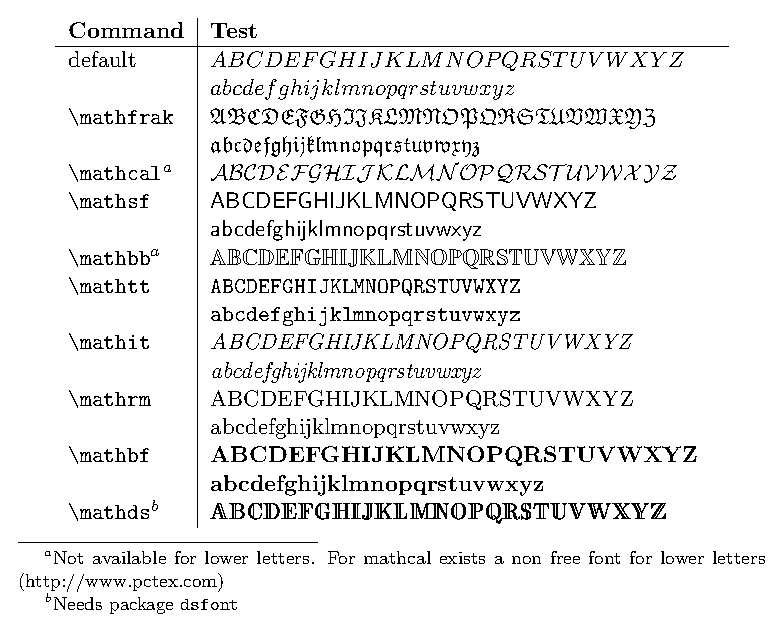
\includegraphics{styles}
\iffalse
\begin{table}[!htb]
\begin{minipage}{\linewidth}
\centering
\begin{tabularx}{.9\linewidth}{l|X}
\textbf{Command} & \textbf{Test}\tabularnewline\hline
default & $ABCDEFGHIJKLMNOPQRSTUVWXYZ$

$abcdefghijklmnopqrstuvwxyz$\tabularnewline
\CMD{mathfrak} &
$\mathfrak{{ABCDEFGHIJKLMNOPQRSTUVWXYZ}}$
$\mathfrak{{abcdefghijklmnopqrstuvwxyz}}$\tabularnewline
\CMD{mathcal}%
\footnote{Not available for lower letters. For mathcal exists a
  non free font for lower letters (http://www.pctex.com)}\addtocounter{mpfootnote}{-1} &
$\mathcal{ABCDEFGHIJKLMNOPQRSTUVWXYZ}$\tabularnewline
\CMD{mathsf}&
$\mathsf{ABCDEFGHIJKLMNOPQRSTUVWXYZ}$
$\mathsf{abcdefghijklmnopqrstuvwxyz}$\tabularnewline

\CMD{mathbb}${}^a$ & $\mathbb{ABCDEFGHIJKLMNOPQRSTUVWXYZ}$\tabularnewline
\CMD{mathtt} & $\mathtt{ABCDEFGHIJKLMNOPQRSTUVWXYZ}$

$\mathtt{abcdefghijklmnopqrstuvwxyz}$\tabularnewline
\CMD{mathit} & $\mathit{ABCDEFGHIJKLMNOPQRSTUVWXYZ}$

$\mathit{abcdefghijklmnopqrstuvwxyz}$\tabularnewline
\CMD{mathrm} & $\mathrm{ABCDEFGHIJKLMNOPQRSTUVWXYZ}$

$\mathrm{abcdefghijklmnopqrstuvwxyz}$\tabularnewline
\CMD{mathbf} & $\mathbf{ABCDEFGHIJKLMNOPQRSTUVWXYZ}$

$\mathbf{abcdefghijklmnopqrstuvwxyz}$\tabularnewline

\CMD{mathds}${}^b$ & $\mathds{ABCDEFGHIJKLMNOPQRSTUVWXYZ}$\tabularnewline
\end{tabularx}
\end{minipage}
\fi
\end{table}

\index{mathfrak@\textbackslash mathfrak}\index{mathsf@\textbackslash mathsf}
\index{mathbb@\textbackslash mathbb}\index{mathcal@\textbackslash mathcal}
\index{mathbf@\textbackslash mathbf}\index{mathit@\textbackslash mathit}
\index{mathrm@\textbackslash mathrm}\index{mathtt@\textbackslash mathtt}
\index{mathds@\textbackslash mathds}\index{double stroke}
\index{dsfont@\texttt{dsfont}}\index{Set symbol}
%\end{comment}

\section{Space}
\subsection{Math typesetting}\label{subsec:mathskip}

\mPar{\CMD{thinmuskip}\\
\CMD{medmuskip}\\
\CMD{thickmuskip}}
\LaTeX\ defines the three math lengths\footnote{For more
information see: \url{http://www.tug.org/utilities/plain/cseq.html}} with the following
values\footnote{see \texttt{\small fontmath.ltx}}:

\begin{lstlisting}
\thinmuskip=3mu
\medmuskip=4mu plus 2mu minus 4mu
\thickmuskip=5mu plus 5mu
\end{lstlisting}

\noindent where \verb|mu| is the abbreviation for \Index{math unit}.
\[
1 \mathrm{mu}= \dfrac{1}{18} \mathrm{em}
\]

\begin{table}[htb]
\centering
\begin{tabular}{ll}
\fboxsep=0pt
\text{default} & $\boxed{f(x)=x^2+3x_0\cdot\sin x}$\\
\CMD{thinmuskip=0mu} & {\thinmuskip=0mu $\boxed{f(x)=x^2+3x_0\cdot\sin x}$}\\
\CMD{medmuskip=0mu} & {\medmuskip=0mu $\boxed{f(x)=x^2+3x_0\cdot\sin x}$}\\
\CMD{thickmuskip=0mu} & {\thickmuskip=0mu $\boxed{f(x)=x^2+3x_0\cdot\sin x}$}\\
all set to zero & {\thickmuskip=0mu\thinmuskip=0mu\medmuskip=0mu $\boxed{f(x)=x^2+3x_0\cdot\sin x}$}\\
\end{tabular}
\caption{The meaning of the math spaces}\label{tab:mathSpaces}
\end{table}

These lengths can have all glue and are
used for the horizontal spacing in math expressions where \TeX{} puts spaces between symbols
and operators. The meaning of these different
horizontal skips is shown in table~\ref{tab:mathSpaces}. For a better typesetting \LaTeX{}
inserts different spaces between the symbols.

\begin{description}
\item[\CIndex{thinmuskip}] space between ordinary and operator atoms
\item[\CIndex{medmuskip}] space between ordinary and binary atoms in display and text styles
\item[\CIndex{thickmuskip}] space between ordinary and relation atoms in display and text styles
\end{description}

\subsection{Additional horizontal spacing}
\mPar{\CMD{thinspace}\\
\CMD{medspace}\\
\CMD{thickspace}\\
\CMD{negthinspace}\\
\CMD{negmedspace}\\
\CMD{negthickspace}}

\begin{table}[!htb]
\def\arraystretch{1.2}
\centering
\begin{tabular}{ll|ll}
\multicolumn{2}{l|}{Positive Space}&\multicolumn{2}{l}{Negative Space}\\\hline
\verb|$ab$|   & $\boxed{a}\boxed{b}$\\
\verb|$a b$|  & $\boxed{a} \boxed{b}$\\
\verb|$a\ b$| & $\boxed{a}\ \boxed{b}$\\
\verb|$a\mbox{\textvisiblespace}b$| & $\boxed{a}\mbox{\textvisiblespace}\boxed{b}$\\
\verb|$a\,b$|\index{,@\textbackslash ,} (\verb|$a\thinspace b$|)\index{thinspace@\textbackslash thinspace} & $\boxed{a}\,\boxed{b}$&
\verb|$a\! b$|\index{negthinspace@\textbackslash negthinspace} & $\boxed{a}\!\boxed{b}$\\
\verb|$a\: b$|\index{:@\textbackslash :} (\verb|$a\medspace b$|)\index{medspace@\textbackslash medspace}&
$\boxed{a}\:\boxed{b}$&
\verb|$a\negmedspace b$|\index{negmedspace@\textbackslash negmedspace} & $\boxed{a}\negmedspace\boxed{b}$\\
\verb|$a\; b$|\index{;@\textbackslash ;} (\verb|$a\thickspace b$|\index{thickspace@\textbackslash thickspace}&
$\boxed{a}\;\boxed{b}$&
\verb|$a\negthickspace b$|\index{negthickspace@\textbackslash negthickspace}&
$\boxed{a}\negthickspace\boxed{b}$\\
\verb|$a\quad b$|\index{quad@\textbackslash quad} & $\boxed{a}\quad\boxed{b}$\\
\verb|$a\qquad b$|\index{qquad@\textbackslash qquad} & $\boxed{a}\qquad\boxed{b}$\\
\verb|$a\hspace{0.5cm}b$|\index{hspace@\textbackslash hspace}& $\boxed{a}\hspace{0.5cm}\boxed{b}$&
\verb|$a\hspace{-0.5cm}b$| & $\boxed{a}\hspace{-0.5cm}\boxed{b}$\\
\verb|$a\kern0.5cm b$|\index{kern@\textbackslash kern} & $\boxed{a}\kern0.5cm \boxed{b}$ & \verb|$a\kern-0.5cm b$| & $\boxed{a}\kern-0.5cm \boxed{b}$\\
\verb|$a\hphantom{xx}b$|\index{hphantom@\textbackslash hphantom} & $\boxed{a}\hphantom{xx}\boxed{b}$\\
\verb|$axxb$| & $\boxed{a}xx\boxed{b}$
\end{tabular}
\caption{Spaces in math mode}\label{cap:Spaces-in-math mode}
\end{table}
%$

LaTeX defines the following short commands:

\begin{verbatim}
\def\>{\mskip\medmuskip}
\def\;{\mskip\thickmuskip}
\def\!{\mskip-\thinmuskip}
\end{verbatim}
In math mode there is often a need for additional tiny spaces between variables,
\eg $L\dfrac{di}{dt}$ written with a tiny space between $L$ and
$\dfrac{di}{dt}$ looks nicer: $L\:\dfrac{di}{dt}$. Table~\ref{cap:Spaces-in-math mode}
shows a list of all commands for horizontal space which can be used
in math mode. The ``space{}'' is seen ``between{}'' the boxed a
and b. For all examples a is \verb+\boxed{a}+ and
b is \verb+\boxed{b}+. The short forms for some
\mPar{\CMD{hspace}\\
\CMD{hphantom}\\
\CMD{kern}} 
spaces may cause problems with other packages. In this case use the
long form of the commands.

\subsection{Problems}\label{space:problems}
Using \CIndex{hphantom} in mathmode depends to on object. \CIndex{hphantom} 
reserves only the space of
the exact width without any additional space. In the following example the second line is
wrong: \verb+& \hphantom{\rightarrow} b\\+. It does not reserve any additional space.

\begin{LTXexample}[width=0.15\linewidth,wide]
\begin{align*}
a & \rightarrow b\\
  & \hphantom{\rightarrow} b\\
  & \mkern\thickmuskip\hphantom{\rightarrow}\mkern\thickmuskip b\\
  & \mathrel{\hphantom{\rightarrow}} b
\end{align*}
\end{LTXexample}

This only works when the math symbol is a mathrel one, otherwise you have to change the
horizontal space to \CIndex{medmuskip} or \CIndex{thinmuskip} or to use an empty group after
the \CIndex{hphantom} command. For more informations
about the math objects look into \verb+fontmath.ltx+ or \PIndex{amssymb} or use the \CIndex{show}
macro, which prints out the type of the mathsymbol, \eg \verb+\show\rightarrow+ with the
output:

\begin{lstlisting}
> \rightarrow=\mathchar"3221.
l.20 \show\rightarrow
\end{lstlisting}

The first digit represents the type:

\begin{tabular}{l@{ : }l}
0 & ordinary\\
1 & large operator\\
2 & binary operation\\ 
3 & relation\\
4 & opening\\
5 & closing\\
6 & punctuation\\ 
7 & variable family
\end{tabular}


%\iffalse
\begingroup
\thinmuskip=3mu
\medmuskip=4mu plus 2mu minus 4mu
\thickmuskip=5mu plus 5mu

\medskip
Grouping a math symbol can change the behaviour in horizontal spacing. Compare
$50\mkern\thinmuskip\times\mkern\thinmuskip10^{12}$ and $50{\times}10^{12}$, the first one is typeset with 
\verb+$50\times10^{12}$+ and the second one with \verb+$50{\times}10^{12}$+.
\endgroup
%\fi
Another possibilty is to use the \PIndex{numprint} package.\footnote{%
\href{ftp://ftp.dante.de/tex-archive/macros/latex/contrib/numprint/}%
{CTAN://macros/latex/contrib/numprint/}}

\subsection{Dot versus comma}\label{subsec:dot-comma}
\mPar{\CMD{mathpunct}\\\CMD{mathord}}%
In difference to a \Index{decimal point} and a \Index{comma} as a marker of thousands a lot of
countries prefer it vice versa. To get the same behaviour the meaning of \Index{dot} and
comma has to be changed:


\begin{align}
1,234,567.89 & \text{ default}\\
1.234.567,89 & \text{ vice versa, wrong spacing}\label{eq:comma}\\
1\mathpunct{.}234\mathpunct{.}567{,}89 & \text{ correct spacing}
\end{align}


\begin{lstlisting}
%\usepackage{amsmath}
1,234,567.89 & \text{ default}\\
1.234.567,89 & \text{ vice versa, wrong spacing}\\
1\mathpunct{.}234\mathpunct{.}567{,}89 & \text{ correct spacing}
\end{lstlisting}

The original definitions from \verb+fontmath.ltx+\footnote{%
Located in \url{texmf/tex/latex/base/}} are

\begin{verbatim}
\DeclareMathSymbol{,}{\mathpunct}{letters}{"3B}
\DeclareMathSymbol{.}{\mathord}{letters}{"3A}
\end{verbatim}

\noindent\CIndex{mathord} and \CIndex{mathpunct} 
can be changed for a documentwide other behaviour. In the above equation~\ref{eq:comma} 
the comma is only set in a pair of braces \verb+{,}+, which is the same as writing 
\verb+\mathord{,}+ because \LaTeX{} handles everything
inside of parenthises as a formula, which gets the same spacing. 

It is also possible to use the package \PIndex{icomma}\footnote{%
\href{ftp://ftp.dante.de/tex-archive/macros/latex/contrib/was/}%
{CTAN:// macros/latex/contrib/was/}} for a documentwide
correct spacing.

\subsection{Vertical whitespace}\label{subsec:vwhitespace}
\subsubsection{Before/after math expressions}\label{subsubsec:displayskip}

There are four predefined lengths, which control the vertical whitespace
of displayed formulas:
\begin{verbatim}
\abovedisplayskip=12pt plus 3pt minus 9pt
\abovedisplayshortskip=0pt plus 3pt
\belowdisplayskip=12pt plus 3pt minus 9pt
\belowdisplayshortskip=7pt plus 3pt minus 4pt
\end{verbatim}
\index{abovedisplayskip@\textbackslash abovedisplayskip}
\index{abovedisplayshortskip@\textbackslash abovedisplayshortskip}
\index{belowdisplayskip@\textbackslash belowdisplayskip}
\index{belowdisplayshortskip@\textbackslash belowdisplayshortskip}
The short skips are used if the formula starts behind the end of the foregoing
last line. Only for demonstration the shortskips
are set to \verb|0pt| in the following examples and the normal skips to 
\verb|20pt| without any glue:

\medskip
\noindent\fbox{\begin{minipage}{\linewidth-2\fboxsep-2\fboxrule}
\abovedisplayshortskip=0pt
\belowdisplayshortskip=0pt
\abovedisplayskip=20pt
\belowdisplayskip=20pt
\noindent The line ends before.
\begin{equation}
f(x) =  \int\frac{\sin x}{x}\,\mathrm{d}x
\end{equation}
\noindent The line doesn't end before the formula.
\begin{equation}
f(x) =  \int\frac{\sin x}{x}\,\mathrm{d}x
\end{equation}
\noindent And the next line starts as usual with some text ...
\end{minipage}}

\medskip
\begin{lstlisting}
\abovedisplayshortskip=0pt
\belowdisplayshortskip=0pt
\abovedisplayskip=20pt
\belowdisplayskip=20pt
\noindent The line ends before.
\begin{equation}
	f(x) =  \int\frac{\sin x}{x}\,\mathrm{d}x
\end{equation}
\noindent The line doesn't end before the formula.
\begin{equation}
	f(x) =  \int\frac{\sin x}{x}\,\mathrm{d}x
\end{equation}
\noindent And the next line starts as usual with some text ...
\end{lstlisting}
%$


\mPar{\texttt{fleqn} class option}%
When using the \verb+fleqn+\index{fleqn@\texttt{fleqn}} classoption for left
aligned equations the math environments \uIndex{equation} 
and \CIndex{[}\ldots\CIndex{]} are typeset as a list. This is the reason why the
vertical space is defined by the length registers for a list, especially
\LIndex{topsep}, instead of \LIndex{abovedisplayskip} and \LIndex{belowdisplayskip}.
This doesn't effect the \UIndex{eqnarray}. 


\subsubsection{Inside math expressions}\label{subsec:vspacing}

\paragraph{\CMD{\textbackslash [<length>]}}
This works inside the math mode in the same way as in the text mode.


\paragraph{\CMD{jot}}\mPar{\CMD{jot}}
The vertical space between the lines for all math expressions which allow multiple
lines  can be changed with the length \LIndex{jot}, which is predefined as

\begin{verbatim}
\newdimen\jot \jot=3pt
\end{verbatim}

The following three formulas show this for the default value, \verb|\setlength\jot{0pt}|  
and \verb|\setlength\jot{10pt}|.

\begin{minipage}{0.3\linewidth}
\begin{eqnarray*}
	y & = & d\\
	y & = & c\frac{1}{x}+d\\
	y & = & b\frac{1}{x^{2}}+cx+d\\
\end{eqnarray*}
\end{minipage}\hfill
\begin{minipage}{0.3\linewidth}
\setlength\jot{0pt}
\begin{eqnarray*}
	y & = & d\\
	y & = & c\frac{1}{x}+d\\
	y & = & b\frac{1}{x^{2}}+cx+d\\
\end{eqnarray*}
\end{minipage}\hfill
\begin{minipage}{0.3\linewidth}
\setlength\jot{10pt}
\begin{eqnarray*}
	y & = & d\\
	y & = & c\frac{1}{x}+d\\
	y & = & b\frac{1}{x^{2}}+cx+d\\
\end{eqnarray*}
\end{minipage}

Defining a new environment with a parameter makes things easier, because changes to the
length are locally.
\begin{lstlisting}
\newenvironment{mathspace}[1]{%
  \setlength{\jot}{#1}%
  \ignorespaces%
}{%
  \ignorespacesafterend%
}
\end{lstlisting}

\paragraph{\CMD{arraystretch}}\cIndex{arraystretch}
\mPar{\CMD{arraystretch}}%
The vertical space between the lines for all math expressions which contain an
\UIndex{array} can be changed with the command
\CIndex{arraystretch}, which is predefined
as
\begin{verbatim}
\renewcommand\arraystretch{1}
\end{verbatim}

Renewing this definition is global to all following math expressions, so it should be used
in the same way as \LIndex{jot}.

\paragraph{\CMD{vskip}}\index{Vertical spacing}\index{Spacing!vertical}
Another spacing for single lines is possible with the \CIndex{vskip} macro:

\begin{LTXexample}[width=0.4\linewidth]
\[
\begin{pmatrix}
0 & 1 & 1 & 0 & 0 & 1 \\
1 & 0 & 0 & 1 & 1 & 0 \\
\noalign{\vskip2pt}
0 & 1 & 1 & 0 & \dfrac{1}{\sqrt{2}} & 1\\
\noalign{\vskip2pt}
1 & 0 & 1 & 0 & 1 & 0 \\
0 & 1 & 0 & 1 & 0 & 1 \\
\end{pmatrix}
\]
\end{LTXexample}



\paragraph{Package \texttt{setspace}}
To have all formulas with another vertical spacing, one can choose
the package \PIndex{setspace} and redefining some of the math macros, \eg

\begingroup
\newcommand*\Array[2][1]{\setstretch{#1}\array{#2}}
\let\endArray\endarray

\begin{lstlisting}
\newcommand*\Array[2][1]{\setstretch{#1}\array{#2}}
\let\endArray\endarray
\end{lstlisting}

\begin{LTXexample}[width=0.25\linewidth]
\[
\begin{Array}[2]{cc}
a =&b\\
a =&b\\
a =&b
\end{Array}
\]

text $\begin{Array}{cc}
a =&b\\
a =&b\\
a =&b
\end{Array}$ text
\end{LTXexample}
\endgroup

\section{Styles}\label{sec:Styles}

\begin{table}[htb]
\newlength\formula
\settowidth{\formula}{$f(t)=\frac{T}{2\pi }\int \frac{1}{\sin \frac{\omega }{t}}dt$}
\begin{tabular}{l|ll}
Mode & Inline & Displayed\\\hline
default & $f(t)=\frac{T}{2\pi}\int\frac{1}{\sin\frac{\omega}{t}}dt$&
\begin{minipage}{\formula}\[
f(t)=\frac{T}{2\pi}\int\frac{1}{\sin\frac{\omega}{t}}dt\]
\end{minipage}\\
\CMD{displaystyle} &
${\displaystyle f(t)=\frac{T}{2\pi}\int\frac{1}{\sin\frac{\omega}{t}}dt}$&
\begin{minipage}{\formula}\[
{\displaystyle f(t)=\frac{T}{2\pi}\int\frac{1}{\sin\frac{\omega}{t}}dt}\]
\end{minipage}\\
\CMD{scriptstyle} &
${\scriptstyle {\textstyle f(t)=\frac{T}{2\pi}\int\frac{1}{\sin\frac{\omega}{t}}dt}}$&
\begin{minipage}{\formula}\[
{\textstyle {\scriptstyle f(t)=\frac{T}{2\pi}\int\frac{1}{\sin\frac{\omega}{t}}dt}}\]
\end{minipage}\tabularnewline
\CMD{scriptscriptstyle} &
${\scriptscriptstyle f(t)=\frac{T}{2\pi}\int\frac{1}{\sin\frac{\omega}{t}}dt}$&
\begin{minipage}{\formula}\[
{\scriptscriptstyle f(t)=\frac{T}{2\pi}\int\frac{1}{\sin\frac{\omega}{t}}dt}\]
\end{minipage}\tabularnewline
\CMD{textstyle} &
${\textstyle f(t)=\frac{T}{2\pi}\int\frac{1}{\sin\frac{\omega}{t}}dt}$&
\begin{minipage}{\formula}\[
{\textstyle f(t)=\frac{T}{2\pi}\int\frac{1}{\sin\frac{\omega}{t}}dt}\]
\end{minipage}
\end{tabular}
\caption{Math styles}\label{cap:Mathstyles}
\end{table}
%$
\makeatletter
\newenvironment{smallequation}[1]{%
  \skip@=\baselineskip
  #1%
  \baselineskip=\skip@
  \equation
}{\endequation \ignorespacesafterend}
\makeatother

This depends on the environment in which they are used. An inline
formula has a default math %
\mPar{\CMD{textstyle}\\
\CMD{displaystyle}\\
\CMD{scriptstyle}\\
\CMD{scripscriptstyle}} fontsize called \CIndex{textstyle},
which is smaller than the one for a display formula (see section~\ref{display}), which is called
\CIndex{displaystyle}.
Beside this predefinition there are two other special fontstyles for
math, \CIndex{scriptstyle} and \CIndex{scriptscriptstyle}.
They are called ``style{}'' in difference to ``size{}'', because
they have a dynamic character, their real fontsize belongs to the
environment in which they are used. A fraction for example is by default in scriptstyle when it is in an
inline formula like this $\frac{a}{b}$, which can be changed to
${\displaystyle \frac{a}{b}}$.
This may be in some cases useful but it looks in general ugly because
the line spacing is too big.
These four styles\index{Style} are predefined and together in a
logical relationship. It is no problem to use the other styles like
\Index{large}, \CIndex{Large}, \ldots\ \textbf{outside} the math environment. 
For example a fraction written with \CIndex{Huge}: {\Huge$\frac{a}{b}$}
(\verb|\Huge$\frac{a}{b}$|). This may cause some problems when you want to write
a displayed formula in another fontsize\index{Fontsize}, because it also affects the interline spacing of
the preceding part of the paragraph.
If you end the paragraph, you get problems with spacing and page breaking
above the equations.  So it is better to declare the font size and then
restore the baselines:
\begin{smallequation}{\tiny}
\int_1^2\,\frac{1}{x^2}\,\mathrm{d}x=0.5
\end{smallequation}
\begin{lstlisting}
\makeatletter
\newenvironment{smallequation}[1]{%
  \skip@=\baselineskip
  #1%
  \baselineskip=\skip@
  \equation
}{\endequation \ignorespacesafterend}
\makeatother

\begin{smallequation}{\tiny}
\int_1^2\,\frac{1}{x^2}\,\mathrm{d}x=0.5
\end{smallequation}
\end{lstlisting}
If you use this the other way round for huge fontsizes, don't forget to load package
\PIndex{exscale} (see section~\vref{sec:exscale}). Also see this section for diffent symbol sizes.



\section{Dots\label{sec:Dots}}

\mPar{\CMD{cdots}\\
\CMD{dots}\\
\CMD{dotsb}\\
\CMD{dotsc}\\
\CMD{dotsi}\\
\CMD{dotsm}\\
\CMD{dotso}\\
\CMD{ldots}\\
\CMD{vdots}}%
In addition to the above decorations there are some more different
dots which are single commands and not by default over/under a letter.
It is not easy to see the differences between some of them. Dots from
lower left to upper right are possible with 
\verb|\reflectbox{$\ddots$}|\index{reflectbox@\textbackslash reflectbox}
\reflectbox{$\ddots$}

\begin{table}[htb]
\centering
\begin{tabular}{*{5}{rc}}
\CMD{cdots}\index{cdots@\textbackslash cdots}&$\cdots$ &
\CMD{ddots}\index{ddots@\textbackslash ddots}&$\ddots$ &
\CMD{dotsb}\index{dotsb@\textbackslash dotsb}&$\dotsb$ &
\CMD{dotsc}\index{dotsc@\textbackslash dotsc}&$\dotsc$ &
\CMD{dotsi}\index{dotsi@\textbackslash dotsi}&$\dotsi$ \\\hline
\CMD{dotsm}\index{dotsm@\textbackslash dotsm}&$\dotsm$ &
\CMD{dotso}\index{dotso@\textbackslash dotso}&$\dotso$ &
\CMD{ldots}\index{ldots@\textbackslash ldots}&$\ldots$ &
\CMD{vdots}\index{vdots@\textbackslash vdots}&$\vdots$
\end{tabular}
\caption{Dots in math mode}
\end{table}



\section{Accents}\label{sec:Accents}

The letter ``a{}'' is only for demonstration.  The table \ref{cap:Accents-in-math mode}
shows all in standard \LaTeX{} available accents and also the ones placed under a character.
With package \PIndex{amssymb} it is easy to define new accents. For
more information see section~\vref{amssymb}  or
other possibilities at section \vref{sec:package-accent}.


\begin{table}[htb]
\makebox[\textwidth]{%
\begin{tabular}{rc|rc|rc}
\CIndex{acute}\index{acute@\textbackslash acute} &$\acute{a}$&
\CIndex{bar}\index{bar@\textbackslash bar}&$\bar{a}$&
\CIndex{breve}\index{breve@\textbackslash breve} & $\breve{a}$\\
\CIndex{bar}\index{bar@\textbackslash bar}&$\bar{a}$&
\CIndex{breve}\index{breve@\textbackslash breve} &$\breve{a}$\tabularnewline
\CIndex{check}\index{check@\textbackslash check} &$\check{a}$&
\CIndex{dddot} \index{dddot@\textbackslash dddot}&$\dddot{a}$&
\CIndex{ddot}\index{ddot@\textbackslash ddot}&$\ddot{a}$\tabularnewline
\CIndex{dot}\index{dot@\textbackslash dot}&$\dot{a}$&
\CIndex{grave}\index{grave@\textbackslash grave}&$\grave{a}$&
\CIndex{hat}\index{hat@\textbackslash hat}&$\hat{a}$\tabularnewline
\CIndex{mathring}\index{mathring@\textbackslash mathring}&$\mathring{a}$&
\CIndex{overbrace}\index{overbrace@\textbackslash overbrace}&$\overbrace{a}$&
\CIndex{overleftarrow}\index{overleftarrow@\textbackslash overleftarrow}&$\overleftarrow{a}$\tabularnewline
\CIndex{overleftrightarrow}\index{overleftrightarrow@\textbackslash overleftrightarrow}&$\overleftrightarrow{a}$&
\CIndex{overline}\index{overline@\textbackslash overline}&$\overline{a}$&
\CIndex{overrightarrow}\index{overrightarrow@\textbackslash overrightarrow}&$\overrightarrow{a}$\tabularnewline
\CIndex{tilde}\index{tilde@\textbackslash tilde}&$\tilde{a}$&
\CIndex{underbar}\index{underbar@\textbackslash underbar}&$\underbar{a}$&
\CIndex{underbrace}\index{underbrace@\textbackslash underbrace}&$\underbrace{a}$\tabularnewline
\CIndex{underleftarrow}\index{underleftarrow@\textbackslash underleftarrow}&$\underleftarrow{a}$&
\CIndex{underleftrightarrow}\index{underleftrightarrow@\textbackslash underleftrightarrow}&
$\underleftrightarrow{a}$&
\CIndex{underline}\index{underline@\textbackslash underline}&$\underline{a}$\tabularnewline
\CIndex{underrightarrow}\index{underrightarrow@\textbackslash underrightarrow}&$\underrightarrow{a}$&
\CIndex{vec}\index{vec@\textbackslash vec}&$\vec{a}$&
\CIndex{widehat}\index{widehat@\textbackslash widehat}&$\widehat{a}$\tabularnewline
\CIndex{widetilde}\index{widetilde@\textbackslash widetilde}&$\widetilde{a}$ & & & &
\end{tabular}%
}
\caption{Accents in math mode}\label{cap:Accents-in-math mode}
\end{table}

The letters \verb+i+ and \verb+j+ can be substituted with the macros \CIndex{imath}
and \CIndex{jmath} when an accents is placed over these letters and the dot should
disappear: $\vec{\imath}\ \dddot{\jmath}$ (\verb+$\vec{\imath}\ \dddot{\jmath}$+).

Accents can be used in different ways, \eg strike a single character with a horizontal line like
\verb+$\mathaccent`-A$+: $\mathaccent`-A$ or \verb+$\mathaccent\mathcode`-A$+: $\mathaccent\mathcode`-A$.
In section~\vref{cancel.sty} is a better solution for more than one character.

\subsection{Over- and underbrackets}
There are no \CIndex{underbracket} and \CIndex{overbracket}
commands in the list of accents. They can be defined in the preamble
with the following code.

\begin{lstlisting}[xleftmargin=-1cm,xrightmargin=-1cm]
\makeatletter
\def\underbracket{%
	\@ifnextchar[{\@underbracket}{\@underbracket [\@bracketheight]}%
}
\def\@underbracket[#1]{%
	\@ifnextchar[{\@under@bracket[#1]}{\@under@bracket[#1][0.4em]}%
}
\def\@under@bracket[#1][#2]#3{%\message {Underbracket: #1,#2,#3}
	\mathop{\vtop{\m@th \ialign {##\crcr $\hfil \displaystyle {#3}\hfil $%
	\crcr \noalign {\kern 3\p@ \nointerlineskip }\upbracketfill {#1}{#2}
     \crcr \noalign {\kern 3\p@ }}}}\limits}
\def\upbracketfill#1#2{$\m@th \setbox \z@ \hbox {$\braceld$}
                  \edef\@bracketheight{\the\ht\z@}\bracketend{#1}{#2}
                  \leaders \vrule \@height #1 \@depth \z@ \hfill
                  \leaders \vrule \@height #1 \@depth \z@ \hfill \bracketend{#1}{#2}$}
\def\bracketend#1#2{\vrule height #2 width #1\relax}
\makeatother
\end{lstlisting}
%$
\begin{enumerate}
\item \verb/\underbrace{...}/ is an often used command:
\begin{eqnarray}
\underbrace{{x^{2}+2x+1}} & = & f(x)\\
\left(x+1\right)^{2}\,\,\,\nonumber
\end{eqnarray}

\item Sometimes an under\textbf{bracket} is needed, which can be used in
	more ways than \verb/\underbrace{...}/.  An example for \verb/\underbracket{...}/:


\begin{eqnarray*}
\textrm{Hate Science  }& \underbracket[0.5pt]{1\rightarrow2\rightarrow3\rightarrow4}
    \underbracket[0.75pt][0.75em]{\rightarrow5\rightarrow6\rightarrow7}
    \underbracket[1pt][1em]{\rightarrow8\rightarrow9\rightarrow10} & \textrm{Love Science}\\
 & \textrm{low}\hspace{1.5cm}\textrm{medium}\hspace{1.5cm}\textrm{high}
 \end{eqnarray*}


\end{enumerate}

\subsubsection{Use of \CMD{underbracket\{...\}}}

The \verb/\underbracket{...}/ command has two optional parameters:

\begin{itemize}
\item the line thickness in any valid latex unit, \eg \verb/1pt/
\item the height of the edge brackets, \eg \verb/1em/
\end{itemize}
using without any parameters gives the same values for thickness and
height as predefined for the \CIndex{underbrace} command.


\vspace{0.3cm}
\begin{center}
\begin{tabular}{|c|c|c|}
\hline
1.& \verb/$\underbracket{foo~bar}$/ & $\underbracket{foo~bar}$ \tabularnewline\hline
2.& \verb/$\underbracket[2pt]{foo~bar}$/ & $\underbracket[2pt]{foo~bar}$ \tabularnewline\hline
3.& \verb/$\underbracket[2pt][1em] {foo~bar}$/& $\underbracket[2pt][1em] {foo~bar}$\tabularnewline\hline
\end{tabular}
\end{center}


\subsubsection{Overbracket}

In addition to the underbracket an overbracket is also useful, which can be used in
more ways than \verb/\overbrace{...}/. For example:


\begin{eqnarray*}
\textrm{Hate Science  }& \overbracket[0.5pt]{1\rightarrow2\rightarrow3\rightarrow4}
    \overbracket[0.75pt][0.75em]{\rightarrow5\rightarrow6\rightarrow7}
    \overbracket[1pt][1em]{\rightarrow8\rightarrow9\rightarrow10} & \textrm{Love Science}\\
 & \textrm{low}\hspace{1.5cm}\textrm{medium}\hspace{1.5cm}\textrm{high}\nonumber
 \end{eqnarray*}


The \verb/\overbracket{...}/ command has two optional parameters:

\begin{itemize}
\item the line thickness in any valid latex unit, \eg \verb/1pt/
\item the height of the edge brackets, \eg \verb/1em/
\end{itemize}
using without any parameters gives the same values for thickness and
height as predefined for the \CIndex{overbrace} command.


\vspace{0.3cm}
\begin{center}\begin{tabular}{|c|c|c|}
\hline
1.&\verb/$\overbracket {foo\ bar}$/ & $\overbracket {foo\ bar}$ \tabularnewline\hline
2.&\verb/$\overbracket[2pt] {foo\ bar}$/ &$\overbracket[2pt] {foo\ bar}$ \tabularnewline\hline
3.&\verb/$\overbracket[2pt] [1em] {foo\ bar}$/&$\overbracket[2pt] [1em] {foo\ bar}$\tabularnewline\hline
\end{tabular}
\end{center}

%$
\subsection{Vectors}

Especially for vectors\index{Vector} there is the package \PIndex{esvect}%
\footnote{\href{http://www.ctan.org/tex-archive/macros/latex/contrib/esvect/}%
	{CTAN://macros/latex/contrib/esvect/}} package, which looks better than the
\CMD{overrightarrow}\index{overrightarrow@\textbackslash overrightarrow}, \eg

\begin{table}[!htb]
\centering
\begin{tabular}{c|c}
\textbackslash{}vv\{...\}&\textbackslash{}overrightarrow\{...\}\tabularnewline\hline
$\vv{a}$ & $\overrightarrow{a}$\tabularnewline
$\vv{abc}$ & $\overrightarrow{abc}$\tabularnewline
$\vv{\imath}$ & $\overrightarrow{\imath}$\tabularnewline
$\vv*{A}{x}$ & $\overrightarrow{A}_{x}$\tabularnewline
\end{tabular}
\caption[Vectors with package \texttt{esvect}]%
    {Vectors with package \texttt{esvect} (in the right column the default one from \LaTeX{})}
\end{table}


Look into the documentation for more details about the package \PIndex{esvect}.

%$
\section{Exponents and indices}\label{sec:exponents}
The two active characters \verb|_| and \verb|^| can only be used in math mode. The
\textbf{following} character will be printed as an index (\verb|$y=a_1x+a_0$|: $y=a_1x+a_0$)
or as an exponent (\verb|$x^2+y^2=r^2$|: $x^2+y^2=r^2$). For more than the next character
put it inside of \verb|{}|, like \verb|$a_{i-1}+a_{i+1}<a_i$|: $a_{i-1}+a_{i+1}<a_i$.

Especially for multiple exponents \index{Multiple exponents}
there are several possibilities. For example:
\begin{equation}
((x^2)^3)^4 = {({(x^2)}^3)}^4 = {\left({\left(x^2\right)}^3\right)}^4
\end{equation}

\begin{lstlisting}
((x^2)^3)^4 =
{({(x^2)}^3)}^4 =
{\left({\left(x^2\right)}^3\right)}^4
\end{lstlisting}

\index{Upright letters}
For variables with both exponent\index{Exponent} and indice index\index{Indice} 
the order is not important, \verb|$a_1^2$| is
exactly the same than \verb|$a^2_1$|: $a_1^2=a^2_1$. By default all exponents and indices
are set as italic characters. It is possible to change this behaviour 
to get upright characters. The following example shows this for the indices.

\bgroup
\begin{LTXexample}[width=4.5cm,preset=\raggedright]
$A_{abc_{xyz}123def}^{abc123def}aa$

\makeatletter
\catcode`\_\active
\def_#1{\sb{\operator@font#1}}
\makeatother

$A_{abc_{xyz}123def}^{abc123def}aa$
\end{LTXexample}
\egroup

\section{Operators}\label{sec:ltxOperators}

They are written in upright font shape and are placed with some additional
space before and after for a better typesetting. With the \AmSmath
package it is possible to define one's own operators\index{Operator} (see
section~\vref{OperatorNames}). Table~\vref{tab:operator} and \vref{tab:operator2} show a list of
the predefined ones for standard \LaTeX{}.

\begin{table}[htb]
\centering
\begin{tabular}{llllll}
\verb+\coprod+  &$\coprod$  &\verb+\bigvee+   &$\bigvee$   &\verb+\bigwedge+&$\bigwedge$\\
\verb+\biguplus+&$\biguplus$&\verb+\bigcap+   &$\bigcap$   &\verb+\bigcup+  &$\bigcup$   \\
\verb+\intop+   &$\intop$   &\verb+\int+      &$\int$      &\verb+\prod+    &$\prod$ \\
\verb+\sum+     &$\sum$     &\verb+\bigotimes+&$\bigotimes$&\verb+\bigoplus+&$\bigoplus$\\
\verb+\bigodot+ &$\bigodot$ &\verb+\ointop+   &$\ointop$   &\verb+\oint+    &$\oint$\\
\verb+\bigsqcup+&$\bigsqcup$&\verb+\smallint+ &$\smallint$
\end{tabular}
\caption{The predefined operators of \texttt{fontmath.ltx}}\label{tab:operator}
\end{table}
The difference between \CIndex{intop} and \CIndex{int} is that the first one has by default
over/under limits and the second subscript/superscript limits. Both can be changed
with the \CIndex{limits} or \CIndex{nolimits} command. The same behaviour happens to the
\CIndex{ointop} and \CIndex{oint} Symbols.

\begin{table}[htb]
\centering
\begin{tabular}{llllll}
\verb+\log+   & $\log$    &\verb+\lg+     & $\lg$      &\verb+\ln+     & $\ln$     \\
\verb+\lim+   & $\lim$    &\verb+\limsup+ & $\limsup$  &\verb+\liminf+ & $\liminf$ \\
\verb+\sin+   & $\sin$    &\verb+\arcsin+ & $\arcsin$  &\verb+\sinh+   & $\sinh$   \\
\verb+\cos+   & $\cos$    &\verb+\arccos+ & $\arccos$  &\verb+\cosh+   & $\cosh$   \\
\verb+\tan+   & $\tan$    &\verb+\arctan+ & $\arctan$  &\verb+\tanh+   & $\tanh$   \\
\verb+\cot+   & $\cot$    &\verb+\coth+   & $\coth$    &\verb+\sec+    & $\sec$    \\
\verb+\csc+   & $\csc$    &\verb+\max+    & $\max$     &\verb+\min+    & $\min$    \\
\verb+\sup+   & $\sup$    &\verb+\inf+    & $\inf$     &\verb+\arg+    & $\arg$    \\
\verb+\ker+   & $\ker$    &\verb+\dim+    & $\dim$     &\verb+\hom+    & $\hom$    \\
\verb+\det+   & $\det$    &\verb+\exp+    & $\exp$     &\verb+\Pr+     & $\Pr$     \\
\verb+\gcd+   & $\gcd$    &\verb+\deg+    & $\deg$     &\verb+\bmod+   & $\bmod$   \\
\verb+\pmod{a}+& $\pmod{a}$
\end{tabular}
\caption{The predefined operators of \texttt{latex.ltx}}\label{tab:operator2}
\end{table}


\makeatletter
\newcommand\foo{\mathop{\operator@font foo}\nolimits}
\makeatother
For more predefined operator names see table~\vref{tab:amsopn}. It is easy 
to define a new operator with
%
\begin{lstlisting}
\makeatletter
\newcommand\foo{\mathop{\operator@font foo}\nolimits}
\makeatother
\end{lstlisting}

Now you can use \verb|\foo| in the usual way:
%
\begin{LTXexample}[width=4cm]
\[ \foo_1^2 = x^2 \]
\end{LTXexample}
In this example \verb|\foo| is defined with \verb|\nolimits|, means 
that limits\index{Limits} are placed in
superscript/subscript mode and not over under. This is still possible with \verb|\limits| in the
definition or the equation:
\begin{LTXexample}[width=4cm]
\[ \foo\limits_1^2 = x^2 \]
\end{LTXexample}

\AmSmath has an own macro for a definition, have a look at section~\vref{OperatorNames}.


\section{Greek letters}\label{sec:greek}
The \AmSmath package simulates a bold font for the greek letters, it writes a 
greek character twice with a small kerning.  The \verb|\mathbf{<character>}| 
doesn't work with lower greek character. See
section \vref{sec:greek-AMS} for the \CIndex{pmb} macro, which makes it possible 
to print bold lower greek\index{Greek} letters. Not all upper case letters have 
own macro names. If there is no difference to the roman font, then the default 
letter is used, \eg A for the upper case of
$\alpha$. Table \ref{tab:greek-letters} shows only those upper case letters 
which have own macro names. Some of the lower case letters have an additional 
\verb|var| option for an alternative.

\bgroup
\tabcolsep=3pt
\begin{longtable}{lclccc}
lower & default &  upper & default & \verb|\mathbf| & \verb|\mathit|\\\hline
\endhead
\verb|\alpha| & $\alpha$ \\
\verb|\beta|  & $\beta$  \\
\verb|\gamma| & $\gamma$
	& \verb|\Gamma| & $\Gamma$ & $\mathbf{\Gamma}$ & $\mathit{\Gamma}$\\
\verb|\delta| & $\delta$
	& \verb|\Delta| & $\Delta$ & $\mathbf{\Delta}$ & $\mathit{\Delta}$\\
\verb|\epsilon|  & $\epsilon$\\
\verb|\varepsilon|  & $\varepsilon$\\
\verb|\zeta|  & $\zeta$\\
\verb|\eta|  & $\eta$ \\
\verb|\theta|  & $\theta$
	& \verb|\Theta| & $\Theta$ & $\mathbf{\Theta}$ & $\mathit{\Theta}$\\
\verb|\vartheta|  & $\vartheta$\\
\verb|\iota|  & $\iota$\\
\verb|\kappa|  & $\kappa$\\
\verb|\lambda| & $\lambda$
	& \verb|\Lambda| & $\Lambda$ & $\mathbf{\Lambda}$ & $\mathit{\Lambda}$\\
\verb|\mu|  & $\mu$ \\
\verb|\nu|  & $\nu$\\
\verb|\xi|  & $\xi$
	& \verb|\Xi| & $\Xi$ & $\mathbf{\Xi}$ & $\mathit{\Xi}$\\
\verb|\pi|  & $\pi$
	& \verb|\Pi| & $\Pi$ & $\mathbf{\Pi}$ & $\mathit{\Pi}$\\
\verb|\varpi|  & $\varpi$ \\
\verb|\rho|  & $\rho$\\
\verb|\varrho|  & $\varrho$\\
\verb|\sigma| & $\sigma$
	& \verb|\Sigma| & $\Sigma$ & $\mathbf{\Sigma}$ & $\mathit{\Sigma}$\\
\verb|\varsigma| & $\varsigma$\\
\verb|\tau|  & $\tau$\\
\verb|\upsilon|  & $\upsilon$
	& \verb|\Upsilon| & $\Upsilon$ & $\mathbf{\Upsilon}$ & $\mathit{\Upsilon}$\\
\verb|\phi|  & $\phi$
	& \verb|\Phi| & $\Phi$ & $\mathbf{\Phi}$ & $\mathit{\Phi}$\\
\verb|\varphi|  & $\varphi$\\
\verb|\chi|  & $\chi$ \\
\verb|\psi|  & $\psi$
	& \verb|\Psi| & $\Psi$ & $\mathbf{\Psi}$ & $\mathit{\Psi}$\\
\verb|\omega| & $\omega$
	& \verb|\Omega| & $\Omega$ & $\mathbf{\Omega}$ & $\mathit{\Omega}$\\[5pt]
\caption{The greek letters}\label{tab:greek-letters}\\
\end{longtable}
\egroup

Bold \Index{greek} letters are possible with the package \PIndex{bm} (see section~\vref{sec:bm})
and if they should also be upright with the package \PIndex{upgreek}:
\index{greek!upright}\index{greek!bold}

\medskip
\verb+$\bm{\upalpha}, \bm{\upbeta} ... $+ $ \bm{\upalpha}, \bm{\upbeta} ... $

A useful definition maybe:

\begin{lstlisting}
\usepackage{upgreek}
\makeatletter
\newcommand{\bfgreek}[1]{\bm{\@nameuse{up#1}}}
\makeatother
\end{lstlisting}

\makeatletter
\newcommand{\bfgreek}[1]{\bm{\@nameuse{up#1}}}
\makeatother
Then 
\verb|$\bfgreek{mu}$| will allow you to type $\bfgreek{mu}$ to obtain an upright boldface $\mu$.



\section{Pagebreaks}
\mPar{\CMD{allowdisplaybreaks}}By default a displayed formula cannot 
have a pagebreak. This makes some sense, but sometimes it gives a better 
typesetting when a pagebreak is possible.

\begin{verbatim}
\allowdisplaybreaks
\end{verbatim}

\CIndex{allowdisplaybreaks} enables \TeX{} to insert pagebreaks into 
displayed formulas whenever a newline command appears.\index{Pagebreak} 
With the command \CIndex{displaybreak} it is also possible to insert a 
pagebreak at any place.

\section{\CMD{stackrel}}

\CIndex{stackrel} puts a character on top of another one which may be important if a
used symbol is not predefined. For example ``$\stackrel{\wedge}{=}$''
(\verb|\stackrel{\wedge}{=}|). \mPar{\CMD{stackrel}}
The syntax is

\begin{lstlisting}
\stackrel{top}{base}
\end{lstlisting}

Such symbols may be often needed so that a macro  definition in the preamble makes some sense:

\begin{lstlisting}
\newcommand{\eqdef}{%
 \ensuremath{\mathrel{\stackrel{\mathrm{def}}{=}}}}
\end{lstlisting}
%
With the \CIndex{ensuremath} command we can use the new \CIndex{eqdef} command in text
and in math mode, \LaTeX{} switches automatically in math mode, which
saves some keystrokes like the following command, which is written
without the delimiters (\texttt{\$...\$}) for the math mode \eqdef ,
only \CMD{eqdef} with a space at the end. In math mode
together with another material it may look like 
$\vec{x}\eqdef\left(x_{1},\ldots,x_{n}\right)$ and as command sequence

\begin{lstlisting}
$\vec{x}\eqdef\left(x_{1},\ldots,x_{n}\right)$
\end{lstlisting}

The fontsize of the top is one size smaller than the one from the
base, but it is no problem to get both the same size, just increase the
top or decrease the base.

\section{\CMD{choose}}

\CIndex{choose}\index{Binom} is like \CIndex{atop}
with delimiters or like \CIndex{frac}
without the fraction line and also with delimiters. It is often used
for binomial coefficients and has the following syntax:\mPar{\CMD{choose}}

\begin{lstlisting}
{above \choose below}
\end{lstlisting}
The two braces are not really important but it is safe to use them.

\begin{equation}
{{m+1 \choose n}}={{m \choose n}}+{{m \choose k-1}}\label{eq:choose}
\end{equation}

\begin{lstlisting}
{{m+1 \choose n}}={{m \choose n}}+{{m \choose k-1}}\label{eq:choose}
\end{lstlisting}


See section~\vref{sub:Binoms} for the \AmSmath equivalents and enhancements.

\section{Color in math expressions}\label{sec:color}
\index{Color}There is no difference in using colored text and colored math expressions. With
\begin{verbatim}
\usepackage{color}
\end{verbatim}

\noindent in the preamble the macro \verb|\textcolor{<color>}{<text or math>}| exists.
\begin{equation}
\textcolor{blue}{f(x)} = \int\limits_1^{\infty}\textcolor{red}{\frac{1}{x^2}}\,\mathrm{d}x=1
\end{equation}
\mPar{\CMD{textcolor}}
\begin{lstlisting}
\begin{equation}
\textcolor{blue}{f(x)} = \int\limits_1^{\infty}\textcolor{red}{\frac{1}{x^2}}\,\mathrm{d}x=1
\end{equation}
\end{lstlisting}

If all math expressions should be printed in the same color, then it is better
to use the \verb+everydisplay+ macro (section~\vref{sec:other}).


\section{Boldmath}\label{sec:boldmath}

\mPar{\CMD{mathversion}\\\CMD{boldmath}\\\CMD{unboldmath}}%
Writing a whole formula in bold\index{boldmath@\textbackslash boldmath} is possible with the command sequence
\CMD{boldmath} \ldots\ \CMD{unboldmath}, which itself must be written in textmode (outside the
formula) or with the command \verb+{\mathversion{bold} ... }+.
\index{mathversion@\textbackslash mathversion}\index{boldmath@\textbackslash
boldmath}\index{unboldmath@\textbackslash unboldmath}

\noindent\begin{minipage}{0.49\linewidth}
\[
\sum_{%
	\makebox[0pt]{$%
		{{\scriptscriptstyle 1\le j\le p\atop {%
		{1\le j\le q\atop 1\le k\le r}}}}%
	$}%
	}a_{ij}b_{jk}c_{ki}
\]
\end{minipage}\hfill
\begin{minipage}{0.49\linewidth}
\boldmath
\[
\sum_{%
	\makebox[0pt]{$%
		{{\scriptscriptstyle 1\le j\le p\atop {%
		{1\le j\le q\atop 1\le k\le r}}}}%
	$}%
	}a_{ij}b_{jk}c_{ki}
\]
\unboldmath
\end{minipage}

\medskip
\begin{lstlisting}
\boldmath
\[
\sum_{%
	\makebox[0pt]{$%
		{{\scriptscriptstyle 1\le j\le p\atop {%
		{1\le j\le q\atop 1\le k\le r}}}}%
	$}%
	}a_{ij}b_{jk}c_{ki}
\]
\unboldmath
\end{lstlisting}

The \verb+\mathversion+ macro defines a math style which is valid for all following
math expressions. If you want to have all math in bold then use this macro instead of
\CIndex{boldmath}. But it is no problem to put \CIndex{mathversion} inside a group to hold
the changes locally.

{\mathversion{bold}%
\begin{equation}
y(x) = ax^3+bx^2+cx+d
\end{equation}}

\begin{lstlisting}
{\mathversion{bold}%
\begin{equation}
y(x) = ax^3+bx^2+cx+d
\end{equation}}
\end{lstlisting}


Single characters inside a formula can be written in bold with \CIndex{mathbf}, 
but only in upright mode, which is in general not useful as shown in 
equation~\ref{eq:bold}. It is better
to use package \PIndex{bm} (see section~\vref{sec:bm}).

\begin{equation}\label{eq:bold}
\sum_{%
	\makebox[0pt]{$%
		{{\scriptscriptstyle 1\le j\le p\atop {%
		{1\le j\le q\atop 1\le k\le r}}}}%
	$}%
	}a_{ij}\mathbf{b_{jk}}c_{ki}
\end{equation}

\subsection[Bold math titles and items]{Bold math expressions as part of titles and items}\label{sec:titleItem}
By default the titles in sections, subsections, a.s.o. are printed in bold. Same for the
\verb|description| environment. The problem is that a math expression in one of these
environments is printed in default font shape, like the following example for a \verb|section| and
\UIndex{description}:

\medskip
\fbox{%
\begin{minipage}{.75\linewidth}
\section*{\thesection\ Function $f(x)=x^2$}
\begin{description}
\item[This is $y=f(x)$] Only a demonstration.
\item[And $z=f(x,y)$] Another demonstration.
\end{description}
\end{minipage}%
}

\medskip
With a redefinition of the \CIndex{section} and 
\CIndex{item} macros it is possible to get everything in bold font.

\medskip
\fbox{%
\begin{minipage}{.75\linewidth}
\let\itemOld\item
\makeatletter
\renewcommand\item[1][]{%
    \def\@tempa{#1}
    \ifx\@tempa\@empty\itemOld\else\boldmath\itemOld[#1]\unboldmath\fi%
}
\makeatother
\section*{\thesection\ \boldmath Function $f(x)=x^2$\unboldmath}
\begin{description}
\item[This is $y=f(x)$] Only a demonstration.
\item[And $z=f(x,y)$] Another demonstration.
\end{description}
\end{minipage}%
}


\medskip
\begin{lstlisting}
\let\itemOld\item
\makeatletter
\renewcommand\item[1][]{%
    \def\@tempa{#1}
    \ifx\@tempa\@empty\itemOld\else\boldmath\itemOld[#1]\unboldmath\fi%
}
\makeatother
\let\sectionOld\section
\renewcommand\section[2][\empty]{%
	\boldmath\sectionOld[#1]{#2}\unboldmath%
}
\end{lstlisting}

\section{Multiplying numbers}
When the dot is used as the decimal marker as in the United States, the preferred sign
for the multiplication of
numbers or values of quantities is a cross (\verb|\times| $\times$ ), not a half-high and
centered dot (\verb|\cdot| $\cdot$ ).

When the comma is used as the decimal marker as in Europe, the preferred sign for the
multiplication of
numbers is the half-high dot. The multiplication of quantity symbols (or numbers in
parentheses or values of
quantities in parentheses) may be indicated in one of the following ways: $ab$,
$a\cdot b$, $a\times b$.

For more information see ``Nist Guide to SI Units -More on Printing and Using Symbols and
Numbers in Scientific and
Technical Documents''\footnote{\url{http://physics.nist.gov/Pubs/SP811/sec10.html}} or
the German DIN 1304, Teil 1.


\section{Other macros}\label{sec:other}
\mPar{\CMD{everymath}\\\CMD{everydisplay}\\\CMD{underline}}%
There are some other macros which are not mentioned in the foregoing text. Here comes
a not really complete list of these macros.
\begin{description}
\item[\CMD{everymath}] \index{everymath@\textbackslash everymath} puts the argument before
any inlined math expression, \eg \verb+\everymath{\displaysize}+. Using this macro doesn't really
make sense, when one is using footnotes because the footnote number is printed as superscript in
inline mathmode and an \CMD{everymath} will be valid, too.
\item[\CMD{everydisplay}] \index{everydisplay@\textbackslash everydisplay} puts  the
argument before any displayed math expression, \eg \verb+\everydisplay{\color{blue}}+.
\item[\CMD{underline}] \index{underline@\textbackslash underline} underlines a math
expression and has to be used inside the math mode.
\[
\underline{F(x)=\int f(x)\,\mathrm{d}x}
\]
\end{description}



\part{\texorpdfstring{\AmSmath}{amsmath} package}\label{par:AMSmath-package}

In general the \AmS packages are at least a collection of three different ones:
\begin{enumerate}
\item \verb|amsmath.sty|
\item \verb|amssymb.sty|
\item \verb|amsfonts.sty|
\end{enumerate}
In the following only the first one is described in detail.

The \AmSmath has the following options:

\bigskip\noindent
\begin{tabularx}{\linewidth}{@{}lX@{}}
\verb+centertags+\index{centertags} & (default) For a split equation, place
equation numbers vertically centered on the total height of the equation.\\\hline
\verb+tbtags+\index{tbtags} & `Top-or-bottom tags' For a split equation,
place equation numbers level with the last (resp. first) line, if
numbers are on the right (resp. left).\\\hline
\verb+sumlimits+\index{sumlimits} & (default) Place the subscripts and superscripts
of summation symbols above and below, in displayed equations. This
option also affects other symbols of the same type -- $\prod$, $\coprod$,
$\bigotimes$, $\bigoplus$, and so forth -- but excluding integrals
(see below).\\\hline
\verb+nosumlimits+\index{nosumlimits} & Always place the subscripts and
superscripts of summation-type symbols to the side, even in displayed
equations.\\\hline
\verb+intlimits+\index{intlimits} & Like sumlimits, but for integral symbols.\\\hline
\verb+nointlimits+\index{nointlimits} & (default) Opposite of intlimits.\\\hline
\verb+namelimits+\index{namelimits} & (default) Like sumlimits, but for
certain `operator names' such as \verb+det+, \verb+inf+, \verb+lim+, \verb+max+, \verb+min+, that traditionally
have subscripts placed underneath when they occur in a displayed equation.\\\hline
\verb+nonamelimits+\index{nonamelimits} & Opposite of namelimits.\\\hline
\end{tabularx}
\bigskip

To use one of these package options, put the option name in the optional
argument, \eg
\verb|\usepackage[intlimits]{amsmath}|. The   %%% ----- Martin -----
\AmSmath also recognises the following options which are normally
selected (implicitly or explicitly) through the \verb|documentclass|
command, and thus need not be repeated in the option list of the \verb|\usepackage{amsmath}| statement.    %%% ----- Martin -----

\bigskip\noindent
\begin{tabularx}{\linewidth}{@{}lX@{}}
\verb+leqno+\index{leqno} & Place equation numbers on the left.\\\hline
\verb+reqno+\index{reqno} & (default) Place equation numbers on the right.\\\hline
\verb+fleqn+\index{fleqn} & Position equations at a fixed indent from the
left margin rather than centered in the text column. \AmSmath defines the
length \CMD{mathindent} and uses it when the equations have only one
tabbing character (\verb+&+).\index{mathindent@\textbackslash mathindent}\\\hline
\end{tabularx}

\bigskip\noindent All math environments are displayed ones, so  there is no special inline
math.

\section{\texttt{align} environments}

There are four different align environments, described in the following
subsections. Their behaviour is shown in table \ref{cap:align}. The symbolic
code for all align environments is:

\begin{lstlisting}
\begin{<name>}
   <name> &= x & x &= x\\
   <name> &= x & x &= x
\end{<name>}
\end{lstlisting}

\begin{table}[htb]
\caption[Comparison between the different align environments]{Comparison between the different align environments
with the same code, where the first three can have an equation number}\label{cap:align}
\begin{align*}
\framebox[0.125\columnwidth]{align} &= \framebox[0.125\columnwidth]{x} & \framebox[0.125\columnwidth]{x}&= \framebox[0.125\columnwidth]{x}\\
\framebox[0.125\columnwidth]{align}&= \framebox[0.1\columnwidth]{x} & \framebox[0.1\columnwidth]{x} &= \framebox[0.1\columnwidth]{x}
\end{align*}

\begin{alignat*}{2}
\framebox[0.125\columnwidth]{alignat} &= \framebox[0.125\columnwidth]{x} & \framebox[0.125\columnwidth]{x} &= \framebox[0.125\columnwidth]{x}\\
\framebox[0.125\columnwidth]{alignat} &= \framebox[0.1\columnwidth]{x} & \framebox[0.1\columnwidth]{x} &= \framebox[0.1\columnwidth]{x}
\end{alignat*}

\begin{flalign*}
\framebox[0.125\columnwidth]{flalign} &= \framebox[0.125\columnwidth]{x} & \framebox[0.125\columnwidth]{x} &= \framebox[0.125\columnwidth]{x}\\
\framebox[0.125\columnwidth]{flalign} &= \framebox[0.1\columnwidth]{x} & \framebox[0.1\columnwidth]{x} &= \framebox[0.1\columnwidth]{x}
\end{flalign*}

\begin{xalignat*}{2}
\framebox[0.125\columnwidth]{xalignat} &= \framebox[0.125\columnwidth]{x} & \framebox[0.125\columnwidth]{x} &= \framebox[0.125\columnwidth]{x}\\
\framebox[0.125\columnwidth]{xalignat} &= \framebox[0.1\columnwidth]{x} & \framebox[0.1\columnwidth]{x} &= \framebox[0.1\columnwidth]{x}
\end{xalignat*}

\begin{xxalignat}{2}
\framebox[0.125\columnwidth]{xxalignat} &= \framebox[0.125\columnwidth]{x} & \framebox[0.125\columnwidth]{x} &= \framebox[0.125\columnwidth]{x}\\
\framebox[0.125\columnwidth]{xxalignat} &= \framebox[0.1\columnwidth]{x} & \framebox[0.1\columnwidth]{x} &= \framebox[0.1\columnwidth]{x}
\end{xxalignat}

\end{table}

In difference to the \UIndex{eqnarray} from standard \LaTeX{} 
(section~\ref{display:eqnarray}),  the ``three'' parts
of one equation \verb+expr.-symbol-expr.+ are divided by only one ampersand    %%% ----- Martin -----
in two parts. In general the ampersand should be before the symbol to get the right spacing, 
\eg \verb+y &= x+. Compare the following three equations, the second one has a wrong spacing.    %%% ----- Martin -----


\noindent
~\hfill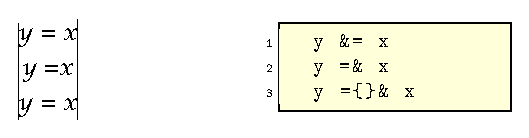
\includegraphics{amsalign}

\iffalse
\begin{minipage}{0.4\linewidth}
\begin{align}
\rnode[lt]{a}{y} &= \rnode[rt]{A}{x}
\end{align}
\vspace*{-3\abovedisplayskip}
\begin{align}
y =& x
\end{align}
\vspace*{-3\abovedisplayskip}
\begin{align}
\rnode[lb]{b}{y} ={}& \rnode[rb]{B}{x}
\end{align}
\ncline[nodesep=-10pt,linewidth=0.1pt]{A}{B}
\ncline[nodesepA=-11pt,nodesepB=-10pt,linewidth=0.1pt]{a}{b}
\end{minipage}
\hfill\begin{minipage}{0.4\linewidth}
\begin{lstlisting}
  y &= x
  y =& x
  y ={}& x
\end{lstlisting}
\end{minipage}
\fi

\subsection{The default \texttt{align} environment}

The \texttt{eqnarray} environment has a not so good spacing between
the cells. Writing the equations no. \ref{eq:2} to \ref{eq:5} with
the \texttt{align} environment gives:

\begin{align}
	y & =d\label{eq:IntoSection}\\
	y & =cx+d\\
	y_{12} & =bx^{2}+cx+d\\
	y(x) & =ax^{3}+bx^{2}+cx+d
\end{align}

\noindent The code looks like:
\begin{lstlisting}
\begin{align}
	y & =d\label{eq:IntoSection}\\
	y & =cx+d\\
	y_{12} & =bx^{2}+cx+d\\
	y(x) & =ax^{3}+bx^{2}+cx+d
\end{align}
\end{lstlisting}

\begin{itemize}
\item The \texttt{align} environment has an implicit \textbf{\{rlrl...\}}
horizontal alignment with a vertical column-alignment, \eg
\begin{LTXexample}[width=0.5\linewidth]
\begin{align*}
  1 & 2 & 3
\end{align*}
\end{LTXexample}

\item A nonumber-version \texttt{\small \textbackslash{}begin\{align{*}\}...\textbackslash{}end\{align{*}\}}
exists.
\item Unnumbered single rows are possible with \CMD{nonumber}.    %%% ----- Martin -----
\item The \texttt{align} environment takes the whole horizontal space if
you have more than two columns:
\begin{align}
y & =d & z & =1\\
y & =cx+d & z & =x+1\\
y_{12} & =bx^{2}+cx+d & z & =x^{2}+x+1\nonumber \\
y(x) & =ax^{3}+bx^{2}+cx+d & z & =x^{3}+x^{2}+x+1
\end{align}

\end{itemize}
The code for this example looks like%
\begin{lstlisting}
\begin{align}
	y & =d & z & =1\\
	y & =cx+d & z & =x+1\\
	y_{12} & =bx^{2}+cx+d & z & =x^{2}+x+1\nonumber \\
	y(x) & =ax^{3}+bx^{2}+cx+d & z & =x^{3}+x^{2}+x+1
\end{align}
\end{lstlisting}

\subsection{\texttt{alignat} environment\label{sec:alignat environment}}
\mPar{\CMD{begin\{align\}\\...\\\CMD{end\{align\}}}}
\renewcommand{\theequation}{%
  \thepart-\arabic{equation}%
}

\begin{leftbar}
>From now the counting of the equation changes. It is introduced with a foregoing command,
which doesn't really make sense, it is only for demonstration:\\
\verb|\renewcommand{\theequation}{\thepart-\arabic{equation}}|.
\end{leftbar}


This means  ``align at several places{}'' and is something like
more than two \verb+align+ environment side by side.
Parameter is the number of the \verb+align+ environments, which
is not important for the user. The
above last \verb+align+ example looks like:

\begin{alignat}{2}
y & =d & z & =1\label{eq:newCounting}\\
y & =cx+d & z & =x+1\\
y_{12} & =bx^{2}+cx+d & z & =x^{2}+x+1\nonumber \\
y(x) & =ax^{3}+bx^{2}+cx+d\quad & z & =x^{3}+x^{2}+x+1\end{alignat}


The parameter was 2 and it is 3 for the following example:    %%% ----- Martin -----

\begin{alignat}{3}
i_{11} & =0.25 & i_{12} & =i_{21} & i_{13} & =i_{23}\nonumber \\
i_{21} & =\frac{1}{3}i_{11} & i_{22} & =0.5i_{12} & i_{23} & =i_{31}\\
i_{31} & =0.33i_{22}\quad & i_{32} & =0.15i_{32}\quad & i_{33} & =i_{11}\end{alignat}


For this example the code is:
\begin{lstlisting}[xleftmargin=-1cm,xrightmargin=-1.5cm]
\begin{alignat}{3}
  i_{11} & =0.25 & i_{12} & =i_{21} & i_{13} & =i_{23}\nonumber\\
  i_{21} & =\frac{1}{3}i_{11} & i_{22} & =0.5i_{12}& i_{23} & =i_{31}\\
  i_{31} & =0.33i_{22}\quad & i_{32} & =0.15i_{32}\quad & i_{33} & =i_{11}
\end{alignat}
\end{lstlisting}

With the \verb+alignat+ environment one can easily align equations vertically
at more than one marker:

\begin{alignat}{3}
   abc &= xxx             &&= xxxxxxxxxxxx &&= aaaaaaaaa \\
   ab  &= yyyyyyyyyyyyyyy &&= yyyy         &&= ab
\end{alignat}
\begin{lstlisting}
\begin{alignat}{3}
   abc &= xxx             &&= xxxxxxxxxxxx &&= aaaaaaaaa \\
   ab  &= yyyyyyyyyyyyyyy &&= yyyy         &&= ab
\end{alignat}
\end{lstlisting}




\begin{itemize}
\item The \texttt{alignat} environment has an implicit \{rlrl...rlrl\}
horizontal alignment with a vertical column alignment.
\item A nonumber-version \texttt{\small
\textbackslash{}begin\{alignat{*}\}...\textbackslash{}end\{alignat{*}\}}
exists.
\item Unnumbered single rows are possible with \CMD{nonumber}.    %%% ----- Martin -----
\end{itemize}

\subsection{\texttt{flalign} environment}\label{ams:flalign}
\mPar{\CMD{begin\{flalign\}\\...\\\CMD{end\{flalign\}}}}This is the new replacement for the \texttt{xalignat} and \texttt{xxalignat}
environments. It is nearly the same as the  \texttt{xalignat} environment, only
more ``out spaced'' and ``left aligned''. 

\begin{LTXexample}[width=0.5\linewidth]
\begin{flalign}
i_{11} & =0.25\nonumber \\
i_{21} & =\frac{1}{3}i_{11}\\
i_{31} & =0.33i_{22}
\end{flalign}
\end{LTXexample}

\medskip
As seen, the equations are not really left aligned, when they have only one
ampersand. In this case \verb+flalign+ has the same behaviour as the \verb+align+
environment.\index{Alignment!left}\index{Indentation}


When there are more than one tabbing characters (\verb+&+), then the equations are
really left aligned. This is also an easy way to get an equation with only one
ampersand left aligned, see equation \ref{eq:leftaligned} below.
\begin{flalign}
i_{11} & =0.25 & i_{12} & =i_{21} & i_{13} & =i_{23}\nonumber \\
i_{21} & =\frac{1}{3}i_{11} & i_{22} & =0.5i_{12} & i_{23} & =i_{31}\\
i_{31} & =0.33i_{22} & i_{32} & =0.15i_{32} & i_{33} & =i_{11}
\end{flalign}
The code looks like:

\begin{lstlisting}[xleftmargin=-1cm,xrightmargin=-1.5cm]
\begin{flalign}
  i_{11} & =0.25 & i_{12} & =i_{21} & i_{13} & =i_{23}\nonumber\\
  i_{21} & =\frac{1}{3}i_{11} & i_{22} & =0.5i_{12}& i_{23} & =i_{31}\\
  i_{31} & =0.33i_{22}\quad & i_{32} & =0.15i_{32}\quad & i_{33} & =i_{11}
\end{flalign}
\end{lstlisting}

\medskip
This environment can be used to mix centered and left aligned\index{Left aligned}
equations without
using the document wide valid option \verb|fleqn|.
\begin{align}\label{eq:centered}
	f(x) & = \int\frac{1}{x^2}\,\mathrm{d}x
\end{align}

\begin{flalign}\label{eq:leftaligned}
	f(x) & = \int\frac{1}{x^2}\,\mathrm{d}x &
\end{flalign}
Equation \ref{eq:leftaligned} is left aligned in fact of the second tabbing
character \verb|&|.

\begin{lstlisting}
\begin{align}\label{eq:centered}
	f(x) & = \int\frac{1}{x^2}\,\mathrm{d}x
\end{align}

\begin{flalign}\label{eq:leftaligned}
	f(x) & = \int\frac{1}{x^2}\,\mathrm{d}x &
\end{flalign}
\end{lstlisting}

Another case is placing text left aligned, whereas the formulas should be right aligned.

\begin{flalign*}
                && 12(x-1)+20(y-3)+14(z-2) &= 0\\
\text{same as } &&               6x+10y+7z &= 0
\end{flalign*}

\begin{lstlisting}
\begin{flalign*}
                && 12(x-1)+20(y-3)+14(z-2) &= 0\\
\text{same as } &&               6x+10y+7z &= 0
\end{flalign*}
\end{lstlisting}


\subsection{\texttt{xalignat} environment}
\mPar{\CMD{begin\{xalignat\}\\...\\\CMD{end\{xalignat\}}}}%
This is an obsolete macro but still supported by the \AmSmath package.
Same as \texttt{alignat} environment, only a little more ``out spaced{}''.
\begin{xalignat}{3}
i_{11} & =0.25 & i_{12} & =i_{21} & i_{13} & =i_{23}\nonumber \\
i_{21} & =\frac{1}{3}i_{11} & i_{22} & =0.5i_{12} & i_{23} & =i_{31}\\
i_{31} & =0.33i_{22} & i_{32} & =0.15i_{32} & i_{33} & =i_{11}
\end{xalignat}
The same code looks like:

\begin{lstlisting}[xleftmargin=-1cm,xrightmargin=-1.5cm]
\begin{xalignat}{3}
  i_{11} & =0.25 & i_{12} & =i_{21} & i_{13} & =i_{23}\nonumber\\
  i_{21} & =\frac{1}{3}i_{11} & i_{22} & =0.5i_{12}& i_{23} & =i_{31}\\
  i_{31} & =0.33i_{22}\quad & i_{32} & =0.15i_{32}\quad & i_{33} & =i_{11}
\end{xalignat}
\end{lstlisting}

\subsection{\texttt{xxalignat} environment}
\mPar{\CMD{begin\{xxalignat\}\\...\\\CMD{end\{xxalignat\}}}}%
Like \texttt{xalignat}  an obsolete macro but still supported by the \AmSmath package.
Same as \texttt{align} environment, only extremely ``out spaced{}'',
therefore no equation number!
\begin{xxalignat}{3}
i_{11} & =0.25 & i_{12} & =i_{21} & i_{13} & =i_{23}\\
i_{21} & =\frac{1}{3}i_{11} & i_{22} & =0.5i_{12} & i_{23} & =i_{31}\\
i_{31} & =0.33i_{22} & i_{32} & =0.15i_{32} & i_{33} & =i_{11}
\end{xxalignat}
The same code looks like:

\begin{lstlisting}[xleftmargin=-1cm,xrightmargin=-1.5cm]
\begin{xxalignat}{3}
  i_{11} & =0.25 & i_{12} & =i_{21} & i_{13} & =i_{23}\nonumber\\
  i_{21} & =\frac{1}{3}i_{11} & i_{22} & =0.5i_{12}& i_{23} & =i_{31}\\
  i_{31} & =0.33i_{22} & i_{32} & =0.15i_{32} & i_{33} & =i_{11}
\end{xxalignat}
\end{lstlisting}


\subsection{\texttt{aligned} environment}\label{sec:aligned}

\mPar{\CMD{begin\{aligned\}\\...\\\CMD{end\{aligned\}}}}In difference to the 
\verb|split| environment (section \vref{split})\index{Split equation}, the 
\verb|aligned| environment allows more than one horizontal alignment but has 
also only one equation number:
%
\begin{equation}
\begin{aligned}
    2x+3 &= 7  &     2x+3-3 &=7-3    \\
    2x   &= 4  & \frac{2x}2 &=\frac42\\
    x    &= 2
\end{aligned}
\end{equation}

\begin{lstlisting}
\begin{equation}
\begin{aligned}
    2x+3 &= 7  &     2x+3-3 &= 7-3    \\
    2x   &= 4  & \frac{2x}2 &= \frac42\\
    x    &= 2
\end{aligned}
\end{equation}
\end{lstlisting}

The \verb|aligned| environment is similar to the \verb|array|\index{array} 
environment, there exists no
starred version and it has only one equation number and has to be part of 
another math environment, which should be \verb|equation| environment. 
The advantage of \verb|aligned| is the much
 better horizontal and vertical spacing.    %%% ----- Martin -----


\subsection{Problems}
When using one of the \verb+align+ environments, there should be no \verb+\\+ at the
end of the last line, otherwise you'll get another equation number for this  
``empty{}'' line:    %%% ----- Martin -----

\begin{LTXexample}[width=0.65\linewidth]
\begin{align}
    2x+3 &= 7\\
\end{align}
\end{LTXexample}

\begin{LTXexample}[width=0.65\linewidth]
\begin{align}
    2x+3 &= 7
\end{align}
\end{LTXexample}
\section{Other environments}


\subsection{\texttt{gather} environment}

\mPar{\CMD{begin\{gather\}\\...\\\CMD{end\{gather\}}}}
This is like a multi line environment with no special horizontal alignment.
All rows are centered and can have an own equation number:
%
\begin{gather}
i_{11}=0.25\\
i_{21}=\frac{1}{3}i_{11}\nonumber \\
i_{31}=0.33i_{22}
\end{gather}
%
For this example the code looks like:
\begin{lstlisting}
\begin{gather}
  i_{11} = 0.25\\
  i_{21} = \frac{1}{3}i_{11}\nonumber\\
  i_{31} =0.33i_{22}
\end{gather}
\end{lstlisting}

\begin{itemize}
\item The \texttt{gather}\index{gather} environment has an implicit \texttt{\{c\}}
horizontal alignment with no vertical column alignment. It is just
like an one column array/table.
\item A nonumber-version \texttt{\small \textbackslash{}begin\{gather{*}\}...\textbackslash{}end\{gather{*}\}}
exists.
Look at section \vref{split} for an example.
\end{itemize}

\subsection{\texttt{gathered} environment}
\mPar{\CMD{begin\{gathered\}[c]\\...\\\CMD{end\{gathered\}}}}

The \verb+gathered+ environment is like the \verb+aligned+ or \verb+alignat+
\index{gathered}\index{aligned}\index{alignat}
environment. They use only so much horizontal space as the widest line needs.
In difference to the \verb+gather+ environment it must be itself inside the
math mode.
%
\begin{align}
\rule{2cm}{1pt}
\begin{gathered}
\quad i_{11}=0.25\\
\quad i_{21}=\frac{1}{3}i_{11}\\
\quad i_{31}=0.33i_{22}
\end{gathered}
\rule{2cm}{1pt}
\end{align}

%
\begin{lstlisting}
\begin{align}
\rule{2cm}{1pt}
\begin{gathered}
\quad i_{11}=0.25\\
\quad i_{21}=\frac{1}{3}i_{11}\\
\quad i_{31}=0.33i_{22}
\end{gathered}
\rule{2cm}{1pt}
\end{align}
\end{lstlisting}
%

The optional argument can be used for setting the vertical alignment which is
by default c (centered). It can also be t for top or b for bottom.

\begin{align}
\rule{1cm}{1pt}
\begin{gathered}[t]
\quad A=a\\
\quad B=b\\
\quad C=c
\end{gathered}
%
\begin{gathered}[c]
\quad A=a\\
\quad B=b\\
\quad C=c
\end{gathered}
%
\begin{gathered}[b]
\quad A=a\\
\quad B=b\\
\quad C=c
\end{gathered}
\ \rule{1cm}{1pt}
\end{align}

\begin{lstlisting}
\begin{align}
\rule{1cm}{1pt}
\begin{gathered}[t]
\quad A=a\\
\quad B=b\\
\quad C=c
\end{gathered}
%
\begin{gathered}[c]
\quad A=a\\
\quad B=b\\
\quad C=c
\end{gathered}
%
\begin{gathered}[b]
\quad A=a\\
\quad B=b\\
\quad C=c
\end{gathered}
\ \rule{1cm}{1pt}
\end{align}
\end{lstlisting}


When using a square bracket as first character inside the environment, then 
everything is ignored by \AmS until a following closing bracket, because \AmS takes this
as an optional argument:
%
\begin{align}
\begin{gathered}
[A]\quad A=a\\
[B]\quad B=b\\
[C]\quad C=c
\end{gathered}
\end{align}
%
\begin{lstlisting}
\begin{align}
\begin{gathered}
[A]\quad A=a\\
[B]\quad B=b\\
[C]\quad C=c
\end{gathered}
\end{align}
\end{lstlisting}
%
The \verb+[A]+ is completely ignored, which can be avoided by using the
optional argument \verb+[c]+ or at least an empty one directly
after the \verb+\begin{gather}+. Another possibility is using the package \verb+empheq+,
which fixes this behaviour by default.
%
\begin{align}
\begin{gathered}[]
[A]\quad A=a\\
[B]\quad B=b\\
[C]\quad C=c
\end{gathered}
\end{align}
%
\begin{lstlisting}
\begin{align}
\begin{gathered}[]
[A]\quad A=a\\
[B]\quad B=b\\
[C]\quad C=c
\end{gathered}
\end{align}
\end{lstlisting}
%


\subsection{\texttt{multline} environment}
\mPar{\CMD{begin\{multline\}\\...\\\CMD{end\{multline\}}}}
This is also like a multi line%
\footnote{It is no typo, the name of the environment is \texttt{multline}, no
missing i here!} environment with a special vertical alignment. The \textbf{first}
row is \textbf{left aligned}, the second and all following ones except
the last one are \textbf{centered} and the \textbf{last} line is \textbf{right
aligned}. It is often used to write extremely long formulas:


\begin{lstlisting}[xleftmargin=-1cm,xrightmargin=-1.5cm]
\begin{multline}
  A = \lim _{n\rightarrow \infty }\Delta x\left( a^{2}+\left( a^{2}+2a\Delta x
          +\left( \Delta x\right) ^{2}\right)\right.\\
  +\left( a^{2}+2\cdot 2a\Delta x+2^{2}\left( \Delta x\right) ^{2}\right)\\
  +\left( a^{2}+2\cdot 3a\Delta x+3^{2}\left( \Delta x\right) ^{2}\right)\\
  + \ldots\\
  \left.+\left( a^{2}+2\cdot (n-1)a\Delta x +(n-1)^{2}\left( \Delta x\right) ^{2}\right) \right)\\
  = \frac{1}{3}\left( b^{3}-a^{3}\right)
\end{multline}
\end{lstlisting}
\begin{multline}
A=\lim_{n\rightarrow\infty}\Delta x\left(a^{2}+\left(a^{2}+2a\Delta x+\left(\Delta x\right)^{2}\right)\right.\label{eq:reset}\\
+\left(a^{2}+2\cdot2a\Delta x+2^{2}\left(\Delta x\right)^{2}\right)\\
+\left(a^{2}+2\cdot3a\Delta x+3^{2}\left(\Delta x\right)^{2}\right)\\
+\ldots\\
\left.+\left(a^{2}+2\cdot(n-1)a\Delta x+(n-1)^{2}\left(\Delta x\right)^{2}\right)\right)\\
=\frac{1}{3}\left(b^{3}-a^{3}\right)
\end{multline}


\begin{figure}[htb]
\begin{multline}
\framebox[0.5\columnwidth]{x}\\
\framebox[0.5\columnwidth]{x}\\
\framebox[0.5\columnwidth]{x}\\
\shoveright{\framebox[0.5\columnwidth]{x}}\\
\framebox[0.5\columnwidth]{x}\\
\framebox[0.5\columnwidth]{x}
\end{multline}
\caption{\texttt{multline} Alignment demo
(the fourth row is shifted to the right with \CMD{shoveright})}
\label{cap:multline-Alignment-Demo}
\end{figure}

\begin{figure}[htb]
\begin{minipage}[c]{0.45\textwidth}%
\fbox{\parbox{\columnwidth}{\begin{multline}
\framebox[0.5\columnwidth]{\textrm{\textbackslash multlinegap=}}\\
\framebox[0.5\columnwidth]{\the\multlinegap}\end{multline}
}}
\end{minipage}%
\hfill{}\begin{minipage}[c]{0.45\textwidth}%
{\setlength{\multlinegap}{0pt}\fbox{\parbox{\columnwidth}{\begin{multline}
\framebox[0.5\columnwidth]{\textbackslash\textrm{multlinegap=}}\\
\framebox[0.5\columnwidth]{\the\multlinegap}\end{multline}
}}}
\end{minipage}%
\caption{\label{cap:multlinegap}Demonstration of \CMD{multlinegap} (default is 0pt)}
\end{figure}



\begin{itemize}
\item A nonumber-version \CMD{begin\{multline{*}\}...}\CMD{end\{multline{*}\}}
exists.
\item By default only the last line (for right equation numbers) or the
first line (for left equation numbers) gets a number, the others can't.
\item The alignment of a single line can be changed with the command
\CMD{shoveright}\index{shoveright@\textbackslash shoveright} (figure \vref{cap:multline-Alignment-Demo})
\item The first line and the last line have a small gap to the text border.%
\footnote{When the first (numbers left) or last line (numbers right) has an
equation number then \CMD{multlinegap} is not used
for these ones, only for the line without a number.} See figure \ref{cap:multlinegap}, where the length of \CMD{multlinegap}\index{multlinegap@\textbackslash multlinegap}
is set to \texttt{0pt} for the right one.
\end{itemize}

\subsubsection{Examples for \texttt{multline}}\label{sec:Specials-for-multline}

With the multline environment the equation~\vref{eq:braces} looks like:

\begin{multline}
\frac{1}{2}\Delta(f_{ij}f^{ij})=2\left(\sum_{i<j}\chi_{ij}(\sigma_{i}-\sigma_{j})^{2}
  +f^{ij}\nabla_{j}\nabla_{i}(\Delta f)+\right.\\
+\left.\nabla_{k}f_{ij}\nabla^{k}f^{ij}+f^{ij}f^{k}\left[2\nabla_{i}R_{jk}-\nabla_{k}R_{ij}
 \right]\right)
\end{multline}
%
which is again a bad typesetting because of the two unequal parentheses.
Each one has a size which is correct for the line but not for the
whole formula. \LaTeX{} accepts only pairs of parentheses for one
line and has an ``empty{}'' parentheses, the dot ``\texttt{\textbackslash{}left.}''
or ``\texttt{\textbackslash{}right.}''{} to get only one of the ``pair{}''.
There are different solutions to get the right size of the parentheses.
One of them is to use the \CMD{vphantom} command,
which reserves the vertical space without any horizontal one, like
a vertical rule without any thickness. The sum symbol from the first
line is the biggest one and responsible for the height, so this one is
the argument of \CMD{vphantom} which has to be
placed anywhere.

\begin{multline}
\frac{1}{2}\Delta(f_{ij}f^{ij})=
	2\left(\sum_{i<j}\chi_{ij}(\sigma_{i}-
	\sigma_{j})^{2}+f^{ij}\nabla_{j}\nabla_{i}(\Delta f)+\right.\\
	\left.+\nabla_{k}f_{ij}\nabla^{k}f^{ij}+
	f^{ij}f^{k}\left[2\nabla_{i}R_{jk}-
	\nabla_{k}R_{ij}\right]\vphantom{\sum_{i<j}}\right)
\end{multline}
%
\begin{lstlisting}[xleftmargin=-1cm,xrightmargin=-1.5cm]
\begin{multline}
\frac{1}{2}\Delta(f_{ij}f^{ij})=
	2\left(\sum_{i<j}\chi_{ij}(\sigma_{i}-
	\sigma_{j})^{2}+f^{ij}\nabla_{j}\nabla_{i}(\Delta f)+\right.\\
	\left.+\nabla_{k}f_{ij}\nabla^{k}f^{ij}+
	f^{ij}f^{k}\left[2\nabla_{i}R_{jk}-
	\nabla_{k}R_{ij}\right]\vphantom{\sum_{i<j}}\right)
\end{multline}
\end{lstlisting}
%
Instead of using the \CMD{vphantom} command it is
also possible to use fixed-width parentheses, which is described in
section \vref{sec:Brackets,-Braces-and}.


A math expression with a very long fraction like the following one, which runs out 
of the margin
could be written as a multiplication to avoid the fraction line.
%
%\begin{LTXexample}[pos=t,xleftmargin=-1cm,xrightmargin=-1.5cm]
\begin{equation}
\frac{\mathrm{d}G_\infty}{\mathrm{d}n}=\frac{\left[1-e^{-pn}\right] 
  \left[Q\left(n\right)-pR\left(n\right)+R'\left(n\right)\right]e^{-pn}
  -\left[-\frac{Q \left(n\right)e^{-pn}}{p}+\frac{Q\left(0\right)}{p}+R
  \left(n\right)e^{-pn} - A\right] pe^{-pn}}{\left({1-e^{-pn}}\right)^2} = 0
\end{equation}
%\end{LTXexample}
%
\begin{lstlisting}[xleftmargin=-1cm,xrightmargin=-1.5cm]
\begin{equation}
\frac{\mathrm{d}G_\infty}{\mathrm{d}n}=\frac{\left[1-e^{-pn}\right] 
  \left[Q\left(n\right)-pR\left(n\right)+R'\left(n\right)\right]e^{-pn}
  -\left[-\frac{Q \left(n\right)e^{-pn}}{p}+\frac{Q\left(0\right)}{p}+R
  \left(n\right)e^{-pn} - A\right] pe^{-pn}}{\left({1-e^{-pn}}\right)^2} = 0
\end{equation}
\end{lstlisting}
%
With the \verb+multline+ environment it can then be split into two or more parts:
%
\begin{LTXexample}[pos=t,xleftmargin=-1cm,xrightmargin=-1.5cm]
\begin{multline}
\frac{\mathrm{d}G_\infty}{\mathrm{d}n} = 
      \frac{1}{\left( {1-e^{-pn}} \right)^2 }\cdot
      \left\{\vphantom{\frac{Q}{p}}% >>>> to get the correct height <<<<<
      \left[ 1-e^{-pn} \right] \left[ Q \left( n \right) - pR 
      \left( n \right) + R'\left( n \right) \right]e^{-pn}\right.\\
    - \left.\left[-\frac{Q \left( n \right) e^{-pn}}{p} + 
    \frac{Q \left( 0 \right)}{p} + R \left( n \right) e^{-pn} 
    - A\right] pe^{-pn}\right\} = 0
\end{multline}
\end{LTXexample}



\subsection{\texttt{split} environment}\label{split}

\mPar{\CMD{begin\{split\}\\...\\\CMD{end\{split\}}}}%
\makeatletter
\@removefromreset{equation}{section}
\makeatother
%
\begin{leftbar}
\noindent From now on the counting of the equations changes. It is introduced with a 
foregoing command, which doesn't really make sense, it is only 
for demonstration: 
\begin{lstlisting}
\makeatletter
\@removefromreset{equation}{section}
\makeatother
\end{lstlisting}
\end{leftbar}


The \verb|split| environment is like the \verb|multline|\index{multline}
or \verb|array| environment for equations longer than the column
width. Just like the array environment and in contrast to \verb|multline|,
\verb|split| can only be used as \textbf{part of another environment}.
\verb|split| itself has no own numbering, this is given by the other
environment. Without an ampersand all lines in the split environment
are right-aligned and can be aligned at a special point by using an
ampersand. In difference to the \verb|aligned| environment (section \vref{sec:aligned}), the \verb|split| 
environment don't permit more than one horizontal alignment.

It is important that the split environment has another behaviour when used inside one of the    %%% ----- Martin -----
``old'' \LaTeX{} environments \verb+\[...\]+ or \verb+\begin{equation}+ \verb+...+\verb+ \end{equation}+, in this
case more than one horizontal alignment tabs are possible.

\hspace*{-\marginparwidth}%
\begin{minipage}{0.5\columnwidth}
\[
\begin{split}
   \framebox[0.35\columnwidth]{x}\\
   \framebox[0.75\columnwidth]{x}\\
   \framebox[0.65\columnwidth]{x}\\
   \framebox[0.95\columnwidth]{x}
\end{split}
\]
\end{minipage}\hfill%
\begin{minipage}{0.5\columnwidth}
\footnotesize\begin{verbatim}
\[
\begin{split}
   \framebox[0.35\columnwidth]{x}\\
   \framebox[0.75\columnwidth]{x}\\
   \framebox[0.65\columnwidth]{x}\\
   \framebox[0.95\columnwidth]{x}
\end{split}
\]
\end{verbatim}
\end{minipage}
\vspace{2ex}

\hspace*{-\marginparwidth}%
\begin{minipage}{0.5\columnwidth}
\[
\begin{split}
   \vec{a} = {}&\framebox[0.35\columnwidth]{x}\\
             &\framebox[0.75\columnwidth]{x}\\
             &\framebox[0.65\columnwidth]{x}\\
             &\framebox[0.95\columnwidth]{x}
\end{split}
\]
\end{minipage}\hspace{1cm}%
\begin{minipage}{0.5\columnwidth}
\footnotesize%
\begin{verbatim}
\[
\begin{split}
   \vec{a} = {}&\framebox[0.35\columnwidth]{x}\\
               &\framebox[0.75\columnwidth]{x}\\
               &\framebox[0.65\columnwidth]{x}\\
               &\framebox[0.95\columnwidth]{x}
\end{split}
\]
\end{verbatim}
\end{minipage}
\vspace{1ex}

The following example shows the \texttt{split} environment as part
of the \texttt{equation} environment:

\begin{equation}
\begin{split}A_{1} & =\left|\int_{0}^{1}(f(x)-g(x))\,\mathrm{d}x\right|+\left|\int_{1}^{2}(g(x)-h(x))\,\mathrm{d}x\right|\\
 & =\left|\int_{0}^{1}(x^{2}-3x)\,\mathrm{d}x\right|+\left|\int_{1}^{2}(x^{2}-5x+6)\,\mathrm{d}x\right|\\
 & =\left|\frac{x^{3}}{3}-\frac{3}{2}x^{2}\right|_{0}^{1}+\left|\frac{x^{3}}{3}-\frac{5}{2}x^{2}+6x\right|_{1}^{2}\\
 & =\left|\frac{1}{3}-\frac{3}{2}\right|+\left|\frac{8}{3}-\frac{20}{2}+12-\left(\frac{1}{3}-\frac{5}{2}+6\right)\right|\\
 & =\left|-\frac{7}{6}\right|+\left|\frac{14}{3}-\frac{23}{6}\right|=\frac{7}{6}+\frac{5}{6}=2\,\textrm{FE}\end{split}
\label{eq:Beispiel-Integral}\end{equation}


\begin{lstlisting}[xleftmargin=-1cm,xrightmargin=-1.5cm]
\begin{equation}
  \begin{split}
    A_{1} & = \left| \int _{0}^{1}(f(x)-g(x))\,\mathrm{d}x\right| +\left|
			\int _{1}^{2}(g(x)-h(x))\,\mathrm{d}x\right| \\
          & = \left| \int _{0}^{1}(x^{2}-3x)\,\mathrm{d}x\right| +\left|
			\int _{1}^{2}(x^{2}-5x+6)\,\mathrm{d}x\right| \\
          & = \left| \frac{x^{3}}{3}-\frac{3}{2}x^{2}\right| _{0}^{1}+
			\left| \frac{x^{3}}{3}-
                \frac{5}{2}x^{2}+6x\right| _{1}^{2}\\
          & = \left| \frac{1}{3}-\frac{3}{2}\right| +\left|
			\frac{8}{3}-\frac{20}{2}+12-
                \left( \frac{1}{3}-\frac{5}{2}+6\right) \right| \\
          & = \left| -\frac{7}{6}\right| +\left| \frac{14}{3}-\frac{23}{6}
			\right| =\frac{7}{6}+\frac{5}{6}=2\, \textrm{FE}
  \end{split}
\end{equation}
\end{lstlisting}

\bigskip{}
The same using the \verb|array| environment with \verb|{rl}|-alignment
instead of \verb|split| gives same horizontal alignment, but another    %%% ----- Martin -----
vertical spacing%
\footnote{Can be changed with \texttt{\textbackslash renewcommand\textbackslash arraystretch\{1.5\}}} and the
symbols are only in scriptsize and not textsize:\footnote{See section \vref{sec:Styles}}    %%% ----- Martin -----

\begin{equation}
\begin{array}{rl}
A_{1} & =\left|\int_{0}^{1}(f(x)-g(x))\,\mathrm{d}x\right|+\left|\int_{1}^{2}(g(x)-h(x))\,\mathrm{d}x\right|\\
 & =\left|\int_{0}^{1}(x^{2}-3x)\,\mathrm{d}x\right|+\left|\int_{1}^{2}(x^{2}-5x+6)\,\mathrm{d}x\right|\\
 & =\left|\frac{x^{3}}{3}-\frac{3}{2}x^{2}\right|_{0}^{1}+\left|\frac{x^{3}}{3}-\frac{5}{2}x^{2}+6x\right|_{1}^{2}\\
 & =\left|\frac{1}{3}-\frac{3}{2}\right|+\left|\frac{8}{3}-\frac{20}{2}+12-\left(\frac{1}{3}-\frac{5}{2}+6\right)\right|\\
 & =\left|-\frac{7}{6}\right|+\left|\frac{14}{3}-\frac{23}{6}\right|=\frac{7}{6}+\frac{5}{6}=2\,\textrm{FE}
 \end{array}
 \end{equation}

Compare the following two examples for typesetting the minus sign. In the first case it
is typeset similiar to the plus character, and in the second example it is typeset
without the additional space for a binary math atom.  

\begin{minipage}{0.49\linewidth}
\begin{align}
\begin{split}
a = {} & -b + c \\
       & -d + e
\end{split}
\end{align}
%
\begin{align}
\begin{split}
a = {} & {-}b + c \\
       & {-}d + e
\end{split}
\end{align}
\end{minipage}\hfill
\begin{minipage}{0.49\linewidth}
\begin{lstlisting}
\begin{align}
\begin{split}
a = {} & -b + c \\
       & -d + e
\end{split}
\end{align}
%
\begin{align}
\begin{split}
a = {} & {-}b + c \\
       & {-}d + e
\end{split}
\end{align}
\end{lstlisting}
\end{minipage}

\begin{itemize}
\item There exists no starred version (\texttt{\textbackslash{}begin\{split{*}\}})    %%% ----- Martin -----
of the \texttt{split} environment.
\end{itemize}


\subsection{\texttt{cases} environment }

This gives support for an often used mathematical construct.\index{cases@\textbackslash cases}
You can also choose the more than once described way to convert some
text into math, like
{\footnotesize\begin{verbatim}
$x=\begin{cases}
 0 & \text{if A=...}\\
 1 & \text{if B=...}\\
 x & \textrm{this runs with as much text as you like,
      but without an automatic linebreak, it runs out
      of page....}
\end{cases}$
\end{verbatim}}
\noindent which gives equation~\vref{eq:cases}. It is obvious what the problem
is.

\begin{eqnarray}
x & = & \begin{cases}
0 & \text{if A=...}\\
1 & \text{if B=...}\\
x & \textrm{this runs with as much text as you like, but without a linebreak, it runs out of page....}\end{cases}\label{eq:cases}\end{eqnarray}


In this case it is better to use a parbox\index{parbox@\textbackslash parbox}
for the text part with a \texttt{flushleft} command for a better view.

\begin{equation}
x=\begin{cases}
0 & \text{if A=...}\\
1 & \text{if B=...}\\
x & \parbox{5cm}{\flushleft this runs with as much text as you like, but without an automatic linebreak, it runs out of page....}\end{cases}\end{equation}



\begin{lstlisting}
\begin{equation}
x=\begin{cases}
  0 & \text{if A=...}\\
  1 & \text{if B=...}\\
  x & \parbox{5cm}{%
      \flushleft%
      this runs with as much text as you like,
      but without an automatic linebreak,
      it runs out of page....}%
\end{cases}
\end{equation}
\end{lstlisting}

\begin{leftbar}
\noindent From now on the counting of the equations changes. It is introduced 
with a foregoing command, which doesn't really make sense, it is only for 
demonstration: 
\begin{lstlisting}
\renewcommand\theequation{\arabic{equation}}
\end{lstlisting}
\end{leftbar}

\renewcommand\theequation{\arabic{equation}}


\subsection{Matrix environments}\label{sec:ams-matrix}
%
\begin{table}[htb]
\centering\begin{tabular}{rcrcrc}
\textbackslash{}Vmatrix\index{Vmatrix@\textbackslash Vmatrix}&
$\begin{Vmatrix}a & b\\
c & d\end{Vmatrix}$&
\textbackslash{}Bmatrix\index{Bmatrix@\textbackslash Bmatrix}&
$\begin{Bmatrix}a & b\\
c & d\end{Bmatrix}$&
\textbackslash{}matrix\index{matrix@\textbackslash matrix}&
$\begin{matrix}a & b\\
c & d\end{matrix}$\tabularnewline
\rule{0pt}{0.85cm}\textbackslash{}vmatrix\index{vmatrix@\textbackslash vmatrix}&
$\begin{vmatrix}a & b\\
c & d\end{vmatrix}$&
\textbackslash{}bmatrix\index{bmatrix@\textbackslash bmatrix}&
$\begin{bmatrix}a & b\\
c & d\end{bmatrix}$&
\textbackslash{}pmatrix\index{pmatrix@\textbackslash pmatrix}&
$\begin{pmatrix}a & b\\
c & d\end{pmatrix}$\tabularnewline[10pt]
&&&&\textbackslash{}smallmatrix\index{smallmatrix@\textbackslash smallmatrix}&
$\begin{smallmatrix}a & b\\
c & d\end{smallmatrix}$
\end{tabular}
\caption{Matrix environments}
\end{table}

All matrix environments can be nested and an element may also contain
any other math environment, so that very complex structures are possible.
By default all cells have a centered alignment, which is often not the best
when having different decimal numbers or plus/minus values. Changing the
alignment to right (not for the \verb+smallmatrix+) is possible with
\mPar{%
\texttt{matrix}\\
\texttt{vmatrix}\\
\texttt{Vmatrix}\\
\texttt{bmatrix}\\
\texttt{Bmatrix}\\
\texttt{pmatrix}\\
\texttt{smallmatrix}%
}%

\begin{lstlisting}
\makeatletter
\def\env@matrix{\hskip -\arraycolsep
  \let\@ifnextchar\new@ifnextchar
  \array{*\c@MaxMatrixCols r}}
\makeatother
\end{lstlisting}

The special matrix environment \verb+smallmatrix+, which decreases
horizontal and vertical space is typeset in scriptstyle. The \verb|smallmatrix|
\index{smallmatrix@\textbackslash smallmatrix} environment makes some sense
in the inline mode to decrease the line height.
For dots over several columns look for \CMD{hdotsfor} in the following section.



\section{Vertical whitespace}\label{sec:ams-whitespace}
See section~\vref{subsec:vwhitespace} for the lengths which control the
vertical whitespace. There is no difference to \AmSmath.

\section{Dots}\label{sec:ams-dots}

In addition to section~\vref{sec:Dots} \AmSmath has two more commands
for dots: \CMD{dddot}\{...\}\footnote{already mentioned in section \ref{sec:Accents}} and \CMD{ddddot}\{...\}
\index{dddot@\textbackslash dddot}\index{ddddot@\textbackslash ddddot}

\verb|$\dddot{y}$|: $\dddot{y}$

\verb|$\ddddot{y}$|: $\ddddot{y}$


Another interesting dot command is \CMD{hdotsfor}\index{hdotsfor@\textbackslash hdotsfor}
with the syntax:

\begin{lstlisting}
\hdotsfor[<spacing factor>]{<number of columns>}
\end{lstlisting}

With the spacing factor the width of the dots can be stretched or
shrinked. The number of columns allows a continuing dotted line over
more columns. Equation \ref{eq:tridiagonal} shows the definition
of a tridiagonal matrix.

\begin{equation}
\underline{A}=\left[\begin{array}{ccccccc}
a_{11} & a_{12} & 0 & \ldots & \ldots & \ldots & 0\\
a_{21} & a_{22} & a_{23} & 0 & \ldots & \ldots & 0\\
0 & a_{32} & a_{33} & a_{34} & 0 & \ldots & 0\\
\vdots & \vdots & \vdots & \vdots & \vdots & \vdots & \vdots\\
\hdotsfor{7}\cr\vdots & \vdots & \vdots & \vdots & \vdots & \vdots & \vdots\\
0 & \ldots & 0 & a_{n-2,n-3} & a_{n-2,n-2} & a_{n-2,n-1} & 0\\
0 & \ldots & \ldots & 0 & q_{n-1,n-2} & a_{n-1,n-1} & a_{n-1,n}\\
0 & \ldots & \ldots & \ldots & 0 & a_{n,n-1} & a_{nn}
\end{array}\right]\label{eq:tridiagonal}
\end{equation}

\begin{lstlisting}[xleftmargin=-1cm,xrightmargin=-1.5cm]
\begin{equation}
\underline{A}=\left[\begin{array}{ccccccc}
a_{11} & a_{12} & 0 & \ldots & \ldots & \ldots & 0\\
a_{21} & a_{22} & a_{23} & 0 & \ldots & \ldots & 0\\
0 & a_{32} & a_{33} & a_{34} & 0 & \ldots & 0\\
\vdots & \vdots & \vdots & \vdots & \vdots & \vdots & \vdots\\
\hdotsfor{7}\cr\vdots & \vdots & \vdots & \vdots & \vdots & \vdots & \vdots\\
0 & \ldots & 0 & a_{n-2,n-3} & a_{n-2,n-2} & a_{n-2,n-1} & 0\\
0 & \ldots & \ldots & 0 & q_{n-1,n-2} & a_{n-1,n-1} & a_{n-1,n}\\
0 & \ldots & \ldots & \ldots & 0 & a_{n,n-1} & a_{nn}
\end{array}\right]
\end{equation}
\end{lstlisting}


\section{\texttt{fraction} commands}\label{sec:ams-fraction}


\subsection{Standard}

Additional to the font size problem described in subsection~\vref{sub:fraction command}
\AmSmath supports some more commands for fractions\index{Fraction}. The \CMD{frac} command
described in \cite{MathGuide}, does no more exist in \AmSmath.    %%% ----- Martin -----

\begin{itemize}
\item The global fraction definition has five parameters\index{genfrac@\textbackslash genfrac}
\index{fraction@\textbackslash frac}
\begin{lstlisting}[xleftmargin=-1em,xrightmargin=-1em]
\genfrac{<left delim>}{<right  delim>}{<thickness>}{<mathstyle>}{<nominator>}{<denominator>}
\end{lstlisting}
where thickness can have any length with a valid unit like \\
\verb|genfrac{}{}{1pt}{}{x^2+x+1}{3x-2}|
$\rightarrow\genfrac{}{}{1pt}{}{x^2+x+1}{3x-2}$
\item \CMD{cfrac}\index{cfrac@\textbackslash cfrac} (continued fraction) which is
by default set in the display mathstyle and useful for fractions like
\begin{equation}
\cfrac{1}{\sqrt{2}+\cfrac{1}{\sqrt{3}+\cfrac{1}{\sqrt{4}+\cfrac{1}{\ldots}}}}\label{cfrac}
\end{equation}
which looks with the default \CMD{frac} command like
\begin{equation}
	\frac{1}{\sqrt{2}+\frac{1}{\sqrt{3}+\frac{1}{\sqrt{4}+\frac{1}{\ldots}}}}
\end{equation}
where the mathstyle decreases for every new level in the fraction.
The \CMD{cfrac} command can be called with an optional
parameter which defines the placing of the nominator, which can be
\texttt{[l]}eft, \texttt{[r]}ight or \texttt{[c]}enter (the default - see
equation~\ref{cfrac}):\\
\begin{minipage}[c]{0.40\textwidth}%
\[
\cfrac[l]{1}{\sqrt{2}+\cfrac[l]{1}{\sqrt{3}+\cfrac[l]{1}{\sqrt{4}+\cfrac[l]{1}{\ldots}}}}
\]
\end{minipage}%
\hfill{}\begin{minipage}[c]{0.40\textwidth}%
\[\cfrac[r]{1}{\sqrt{2}+\cfrac[r]{1}{\sqrt{3}+\cfrac[r]{1}{\sqrt{4}+\cfrac[r]{1}{\ldots}}}}\]
\end{minipage}%

\item \CMD{dfrac}\index{dfrac@\textbackslash dfrac}
which takes by default the displaystyle\index{displaystyle@\textbackslash displaystyle}, so that
fractions in inline mode $\dfrac{1}{2}$ have the same size than in
display mode.
\item \CMD{tfrac}\index{tfrac@\textbackslash tfrac} (vice versa to \CMD{dfrac}) which takes by default
the scriptstyle\index{scriptstyle@\textbackslash scriptstyle}, so that fractions in display
mode have the same size than in inline mode.
\end{itemize}

\[\tfrac{2}{3} \text{\hspace{0.5cm}\CMD{tfrac\{2\}\{3\}}} \]
\[\frac{2}{3} \text{\hspace{0.5cm}\CMD{frac\{2\}\{3\}}} \]


\subsection{Binoms}\label{sub:Binoms}

\mPar{\CMD{binom}\\\CMD{dbinom}\\\CMD{tbinom}}They are like fractions without a rule and its syntax is different
to the \CMD{choose} command from standard \LaTeX{}
(see section \vref{sub:fraction command}). \AmSmath{} provides three
different commands for binoms just like the ones for fractions.

\begin{table}[htb]
\centering%
\begin{tabular}{lcl}
Command & Inlinemath & Displaymath\tabularnewline
\hline
\texttt{\textbackslash{}binom\{m\}\{n\}} & $\binom{m}{n}$&
${\displaystyle \binom{m}{n}}$\tabularnewline
\texttt{\rule{0pt}{0.75cm}\textbackslash{}dbinom\{m\}\{n\}}&
$\dbinom{m}{n}$&
${\displaystyle \dbinom{m}{n}}$\tabularnewline
\texttt{\rule{0pt}{0.5cm}\textbackslash{}tbinom\{m\}\{n\}}&
$\tbinom{m}{n}$&
${\displaystyle \tbinom{m}{n}}$\tabularnewline
\end{tabular}
\caption{binom commands}
\end{table}


\section{Roots}\label{sec:Roots-ams}

The typesetting for roots\index{uproot@\textbackslash uproot} is sometimes not
the best. Some solutions for better typesetting are %
\mPar{\CMD{leftroot}\\\CMD{uproot}}%
described in section~\vref{sec:Roots} for standard \LaTeX{}. \AmSmath
has some more commands for the $n$-th root:

\begin{lstlisting}
\sqrt[\leftroot{<number>}\uproot{<number>}<root>]{< ... >}
\end{lstlisting}

\noindent \verb+<number>+ indicates a value for the points%
\footnote{In PostScript units (bp -- Big Points).} of which the root can be
adjusted to the left and/or to the top, \eg
$\sqrt[k_n]{a}$ (\verb+$\sqrt[k_n]{a}$+) has a too deep exponent, whereas $\sqrt[\uproot{2}k_n]{a}$ \verb+$\sqrt[\uproot{2}k_n]{a}$+ looks nicer.



\subsection{Roots with \CMD{smash} command}

\mPar{\CMD{smash}}The default for a root\index{Root} with $\lambda_{k_{i}}$ as root
argument looks like $\sqrt{\lambda_{k_{i}}}$, which may be not the    %%% ----- Martin -----
best typesetting. It is possible to reduce the lowest point of the root
to the baseline with the \CMD{smash} command: $\sqrt{\lambda_{k_{i}}}\xrightarrow{\text{with \textbackslash smash}}\sqrt{\smash[b]{\lambda_{k_{i}}}}$


The syntax of the \CMD{smash} command%
\footnote{In \texttt{latex.ltx} \CMD{smash} is defined without an optional argument.} renewed by the \AmSmath  package is    %%% ----- Martin -----

\begin{lstlisting}
\smash[<position>]{<argument>}
\end{lstlisting}
The optional argument for the position can be:

\begin{description}
\item [t]keeps the bottom and annihilates the top
\item [b]keeps the top and annihilates the bottom
\item [tb]annihilates top and bottom (the default)
\end{description}

\section{Accents}\label{amssymb}

With the macro \verb|\mathaccent| it is easy to define new accent types, for example

\begin{lstlisting}
\def\dotcup{$\mathaccent\cdot\cup$}
\end{lstlisting}

$\mathaccent\cdot\cup$

\def\curvearrowleftright{%
	\ensuremath{%
		\mathaccent\curvearrowright{\mkern-5mu\curvearrowleft}%
	}%
}

Overwriting of two symbols is also possible:

{\huge
$\curvearrowleft\curvearrowright\curvearrowleftright$}

In this case the second symbol has to be shifted to the left for a length    %%% ----- Martin -----
of $5mu$ (mu: math unit\index{Math unit}).

\begin{lstlisting}
\def\curvearrowleftright{%
	\ensuremath{%
		\mathaccent\curvearrowright{\mkern-5mu\curvearrowleft}%
	}%
}
\end{lstlisting}

For other possibilities to define new accents see section \vref{sec:package-accent}.    %%% ----- Martin -----

\section{\CMD{mod} command}

In standard \LaTeX{} the modulo command is not an operator, though    %%% ----- Martin -----
it is often used in formulas. \AmSmath provides two (three) different
commands for modulo, which are listed in tabular~\vref{cap:The-modulo commands}.

\begin{itemize}
\item They all insert some useful space before and behind the mod-operator.
\end{itemize}

\begin{table}[htb]
\centering\begin{tabular}{rrl}
a\textbackslash{}mod\{n\^{}2\}=b&
$\rightarrow$&
$a\mod{n^{2}}=b$\tabularnewline
a\textbackslash{}pmod\{n\^{}2\}=b&
$\rightarrow$&
$a\pmod{n^{2}}=b$\tabularnewline
a\textbackslash{}pod\{n\^{}2\}=b&
$\rightarrow$&
$a\pod{n^{2}}=b$\tabularnewline
\end{tabular}
\caption{\label{cap:The-modulo commands}The modulo commands and their meaning}
\end{table}



\section{Equation numbering\label{sec:Equation-numbering}}

See section \vref{sub:Equationnumbering} for equation numbering\index{Equation!numbering}.
It is mostly the %
\mPar{\textbackslash{}numberwithin%
}same, only one command is new to \AmSmath. If you want
a numbering like ``\ref{eq:IntoSection}{}'' then write either in the preamble    %%% ----- Martin -----
or like this example anywhere in your doc:

\begin{lstlisting}
\numberwithin{equation}{section}
\end{lstlisting}

\begin{leftbar}
\numberwithin{equation}{section}From now on the numbering looks like    %%% ----- Martin -----
equation \vref{eq:IntoSection}. For the book-class you can get the
same for chapters.
\end{leftbar}

If you want to get rid of the parentheses then write in the preamble:    %%% ----- Martin -----

\begin{lstlisting}
\makeatletter
\def\tagform@#1{\maketag@@@{\ignorespaces#1\unskip\@@italiccorr}}
\makeatother
\end{lstlisting}

Now the following four subequation numbers have no parentheses.




\makeatletter
\let\oldTagForm\tagform@
\def\tagform@#1{\maketag@@@{\ignorespaces#1\unskip\@@italiccorr}}
\makeatother

\subsection{Subequations}\label{ams:subeqn}

Amsmath supports this with the environment \verb|subequation|\index{Subequations}.
For example:
\begin{subequations}
\begin{align}
y & =  d\\
y & =  cx+d\\
y & =  bx^{2}+cx+d\\
y & =  ax^{3}+bx^{2}+cx+d
\end{align}
\end{subequations}

\begin{lstlisting}
\begin{subequations}
\begin{align}
y & =  d\\
y & =  cx+d\\
y & =  bx^{2}+cx+d\\
y & =  ax^{3}+bx^{2}+cx+d
\end{align}
\end{subequations}
\end{lstlisting}

\makeatletter
\let\tagform@\oldTagForm
\makeatother


Inside of subequations only complete other environments (\texttt{\textbackslash{}begin\{...\}
... \textbackslash{}end\{...\}}) are possible.

\begin{lstlisting}
\renewcommand{\theequation}{%
  \theparentequation{}-\arabic{equation}%
}
\end{lstlisting}

\begin{subequations}
\renewcommand{\theequation}{%
  \theparentequation -\arabic{equation}%
}%
\begin{align}
y & =  d\\
y & =  cx+d\label{eq:subequation-neu}\\
y & =  bx^{2}+cx+d\\
y & =  ax^{3}+bx^{2}+cx+d
\end{align}
\end{subequations}

A ref to a subequation is possible like the one to equation \ref{eq:subequation-neu}.
The environment chooses the same counter ``\texttt{equation}''
but saves the old value into ``\texttt{parentequation}''.

\newcounter{mySubCounter}
\newcommand{\twocoleqn}[2]{
    \setcounter{mySubCounter}{0}%
    \let\OldTheEquation\theequation%
    \renewcommand{\theequation}{\OldTheEquation\alph{mySubCounter}}%
    \noindent%
    \begin{minipage}{.49\textwidth}
          \begin{equation}\refstepcounter{mySubCounter}
            #1
        \end{equation}
    \end{minipage}\hfill%
    \addtocounter{equation}{-1}%
    \begin{minipage}{.49\textwidth}
        \begin{equation}\refstepcounter{mySubCounter}
            #2
        \end{equation}
    \end{minipage}
    \let\theequation\OldTheEquation
}

It is also possible to place two equations side by side with counting as subfigures:

\twocoleqn{y=f(x)}{y=f(z)}

\vspace{1ex}
In this case, the \AmSmath internal subfigure counter cannot be used and an own
counter has to be defined:

\begin{lstlisting}
\newcounter{mySubCounter}
\newcommand{\twocoleqn}[2]{
    \setcounter{mySubCounter}{0}%
    \let\OldTheEquation\theequation%
    \renewcommand{\theequation}{\OldTheEquation\alph{mySubCounter}}%
    \noindent%
    \begin{minipage}{.49\textwidth}
          \begin{equation}\refstepcounter{mySubCounter}
            #1
        \end{equation}
    \end{minipage}\hfill%
    \addtocounter{equation}{-1}%
    \begin{minipage}{.49\textwidth}
        \begin{equation}\refstepcounter{mySubCounter}
            #2
        \end{equation}
    \end{minipage}%
    \let\theequation\OldTheEquation
}
[ ... ]
\twocoleqn{y=f(x)}{y=f(z)}
\end{lstlisting}


\section{Labels and tags}\label{sec:Labels-and-Tags}

For the \CMD{label} command\index{label@\textbackslash label} \mPar{\textbackslash{}tag%
}
see section \vref{sec:Labels}, it is just the same behaviour. \AmSmath
allows to define own single ``equation numbers\index{Equation number}''
with the \CMD{tag} command. 
\begin{align}
f(x) & =a\tag{linear}\label{eq:linear}\\
g(x) & =\,\mathrm{d}x^{2}+cx+b\tag{quadratic}\label{eq:quadratic}\\
h(x) & =\sin x\tag*{trigonometric}
\end{align}

\begin{lstlisting}
\begin{align}
f(x) & =a\tag{linear}\label{eq:linear}\\
g(x) & =\,\mathrm{d}x^{2}+cx+b\tag{quadratic}\label{eq:quadratic}\\
h(x) & =\sin x\tag*{trigonometric}
\end{align}
\end{lstlisting}

\begin{itemize}
\item The \CMD{tag} command is also possible for unnumbered
equations, \LaTeX{} changes the behaviour when a tag is detected.
\item There exists a starred version \verb|\tag{*}{...}|,    %%% ----- Martin -----
which supresses any annotations like parentheses for equation numbers\index{Equation!number}.
\item There exist two package options for tags, \verb|ctagsplit|\index{ctagsplit}    %%% ----- Martin -----
and \verb|righttag|\index{righttag} (look at the beginning of this
part on page~\pageref{par:AMSmath-package}).
\end{itemize}


\section{Limits}\label{sec:limit-AMS}

By default the sum/prod has the limits above/below and the integral
at the side. To get the same behaviour for all symbols which can have
limits load the package \AmSmath in the preamble as    %%% ----- Martin -----

\begin{lstlisting}
\usepackage[sumlimits,intlimits]{amsmath}
\end{lstlisting}

There exist also options for the vice versa (see page~\pageref{par:AMSmath-package}).    %%% ----- Martin -----
See also Section~\ref{sec:misc-AMS} for the additional commands \CMD{underset} and \CMD{overset}.



\subsection{Multiple limits}

For general information about limits\index{Limits} read section
\vref{sub:Limits-Inline}. Standard \LaTeX{} provides the \texttt{\textbackslash{}atop}\index{atop@\textbackslash atop} command
for multiple limits (section \vref{sub:Multiple-Limits}). \AmSmath \mPar{\textbackslash{}substack%
}
has an additional command for that, which
can have several lines with the following syntax:
\mPar{\CMD{begin\{Sb\}}\\...\\\CMD{end\{Sb\}}\\\CMD{begin\{Sp\}}\\...\\\CMD{end\{Sp\}}%
}

\begin{lstlisting}
\substack{...\\...\\...}
\end{lstlisting}

The environments described in \cite{MathGuide}

\begin{lstlisting}
\begin{Sb} ... \end{Sb}
\begin{Sp} ... \end{Sp}
\end{lstlisting}
are obsolete and no more part of \AmSmath.

The example equation \vref{eq:atop} with the \CMD{substack}\index{substack@\textbackslash substack} command
looks like:

\begin{equation}\label{eq:multlimits}
\sum_{\substack{1\le i\le p\\
1\le j\le q\\
1\le k\le r}
}a_{ij}b_{jk}c_{ki}
\end{equation}


Insert these limits in the following way:
\begin{lstlisting}
\begin{equation}
	\sum_{%
		\substack{1\le i\le p\\
			1\le j\le q\\
			1\le k\le r}
		}%
	a_{ij}b_{jk}c_{ki}
\end{equation}
\end{lstlisting}

\subsection{Problems}\label{subsec:ams-limits}

There are still some problems with limits and the following math
expression. For example:

\[
X = \sum_{1\le i\le j\le n}X_{ij}
\]
\begin{lstlisting}
\[
X = \sum_{1\le i\le j\le n}X_{ij}
\]
\end{lstlisting}

\noindent does not look nice because of the long limit. Using a
\CMD{makebox} also does not really solve the problem, because
\CMD{makebox} is in \TeX{} horizontal mode and knows nothing about
the appropriate math font size, because limits have a smaller font size.
It is better to define a \CMD{mathclap}\index{mathclap@\textbackslash mathclap} macro, similiar to the two
macros \CMD{llap} and \CMD{rlap} and uses the also new defined \CMD{mathclap} macro\index{clap@\textbackslash clap}:

\begin{lstlisting}
\def\mathllap{\mathpalette\mathllapinternal}
\def\mathllapinternal#1#2{%
	\llap{$\mathsurround=0pt#1{#2}$}% $
}
\def\clap#1{\hbox to 0pt{\hss#1\hss}}
\def\mathclap{\mathpalette\mathclapinternal}
\def\mathclapinternal#1#2{%
	\clap{$\mathsurround=0pt#1{#2}$}%
}
\def\mathrlap{\mathpalette\mathrlapinternal}
\def\mathrlapinternal#1#2{%
	\rlap{$\mathsurround=0pt#1{#2}$}% $
}
\end{lstlisting}


Now we can write limits which have a boxwidth of 0pt and the right font
size and the following math expression appears just behind the symbol:

\[
X = \sum_{\mathclap{1\le i\le j\le n}}X_{ij}
\]
\begin{lstlisting}
\[
X = \sum_{\mathclap{1\le i\le j\le n}}X_{ij}
\]
\end{lstlisting}

Another problem occurs when having operators with stacked limits in braces:\index{substack@\textbackslash substack}
\index{Braces!Problems}
\index{Stacked limits}
\begin{align}
\left[\sum_{\substack{i,j\\i>j}} \dots \right]
\end{align}

This case is not easy to handle when some other math expressions are around the braces
which should be on the same baseline. However, the following may help in some cases
to get better looking braces.

\begin{LTXexample}[width=0.45\linewidth,wide]
\begin{align}
foo \left[\begin{array}{@{}c@{}}
    \displaystyle\sum_{\substack{i,j\\i>j}} \dots
  \end{array}\right] bar
\end{align}
\end{LTXexample}


\subsection{\CMD{sideset}}

This is a command for a very special purpose, to combine over/under
limits with superscript/subscripts for \mPar{\CMD{sideset}}the
sum-symbol. For example: it is not possible to place the prime
for the equation \ref{eq:sideset} near to the sum\index{sum@\textbackslash sum} symbol,
because it becomes an upper limit when writing without an preceeding \verb|{}|.
\begin{equation}
\sum_{n<k\atop n\ \textrm{odd}}{}'nE_{n}\label{eq:sideset}
\end{equation}

The command \CMD{sideset}\index{sideset@\textbackslash sideset}
has the syntax

\begin{lstlisting}
\sideset{<before>}{<behind>}
\end{lstlisting}

It can place characters on all four corners of the sum-symbol:
\[
\sideset{_{LowerLeft}^{UpperLeft}}{_{LowerRight}^{UpperRight}}\sum_{B}^{T}
\]

\begin{lstlisting}
\[
\sideset{_{LowerLeft}^{UpperLeft}}{_{LowerRight}^{UpperRight}}\sum_{B}^{T}
\]
\end{lstlisting}

Now it is possible to write the equation \ref{eq:sideset} in a proper
way with the command \verb|\sideset{}{'}| before
the sum symbol:
\begin{equation}
\sideset{}{'}\sum_{n<k\atop n\ \textrm{odd}}nE_{n}
\end{equation}


\section{Operator names}\label{OperatorNames}

\mPar{\CMD{operatorname}}%
By default variables are written in italic\index{Italic} and operator
names\index{Operator!names} in upright mode, like $y=\sin(x)$.%
\footnote{See section \vref{sec:ltxOperators}, where all the standard \LaTeX{}    %%% ----- Martin -----
known operator names are listed. Package \AmSmath has
some more (see documentation).} This happens only for the known operator names, but creating a new
one is very easy with:

\begin{lstlisting}
\newcommand{\mysin}{\operatorname{mysin}}
\end{lstlisting}

Now \CMD{mysin} is also written in upright mode
$y=\mysin(x)$ and with some additional space before and behind.

It is obvious, that only those names can be defined as new operator
names which are not commands in another way. Instead of using the
new definition as an operator, it is also possible to use the text
mode. But it is better to have all operators of the same type, so that
changing the style will have an effect for all operators.

\mPar{\CMD{operatornamewithlimits}}%
The new defined operator names cannot have limits\index{Limits}, only
superscript/subscript is possible. \verb+amsopn.sty+ has an additional command
\CMD{operatornamewithlimits}\index{operatornamewithlimits@\textbackslash operatornamewithlimits},
which supports over/under limits like the one from \CMD{int}
or \CMD{sum}.

\mPar{\CMD{mathop}}
It is also possible to use the macro \verb+\mathop+ to declare anything
as operator, like
\[ \sideset{_1}{}{\mathop{\mathrm{B}}} \]
\begin{lstlisting}
\[ \sideset{_1}{}{\mathop{\mathrm{B}}} \]
\end{lstlisting}
With this definition it is possible to use \CMD{sideset} for a forgoing index, which
is only possible for an operator.

For a real \LaTeX{} definition have a look at section \vref{sec:ltxOperators}.


\section{Text in math mode}\label{sec:Text-in-math mode}

If you need complex structures between formulas, look also at section \ref{sec:verticalAlignment}.

\subsection{\CMD{text} command}
\mPar{%
\CMD{text}\\
\CMD{mbox}\\
\CMD{textnormal}\\
\CMD{mathrm}%
}%
This is the equivalent command to \CMD{mathrm}\index{mathrm@\textbackslash mathrm}
or \CMD{mbox}\index{mbox@\textbackslash mbox}
from the standard \LaTeX{} (section~\vref{sec:Text}) with the exception, that \CMD{mathrm}
always uses the roman font and \CMD{text} the actual one and that the font size is different
when used in super- and subscript. 

For example: $\boxed{f(x)=x\quad\text{this was math}}$.

\bigskip
{\sffamily\huge
$A^{\mbox{text}}_{\mbox{text}}$\quad
$A^{\text{text}}_{\text{text}}$\quad
$A^{\textnormal{text}}_{\textnormal{text}}$\quad
$A^{\mathrm{text}}_{\mathrm{text}}$
}
\medskip
\begin{lstlisting}
$\boxed{f(x)=x\quad\text{this was math}}$

{\sffamily\huge
$A^{\mbox{text}}_{\mbox{text}}$\quad
$A^{\text{text}}_{\text{text}}$\quad
$A^{\textnormal{text}}_{\textnormal{text}}$\quad
$A^{\mathrm{text}}_{\mathrm{text}}$ 
}
\end{lstlisting}

The \verb+\text+ macro can be used at any place and can be in some cases a better
solution as \verb+\intertext+ (see section~\ref{subsec:intertext}).

\begin{flalign*}
             && 12(x-1) + 20(y-3) + 14(z-2) & = 0 &&\\
  \text{and} &&               6x + 10y + 7z & = 0  &&
\end{flalign*}

\begin{align}
            && 12(x-1) + 20(y-3) + 14(z-2) & = 0\\
  \text{and} &&               6x + 10y + 7z & = 0 
\end{align}

\begin{lstlisting}
\begin{flalign*}
             && 12(x-1) + 20(y-3) + 14(z-2) & = 0 &&\\
  \text{and} &&               6x + 10y + 7z & = 0  &&
\end{flalign*}

\begin{align}
            && 12(x-1) + 20(y-3) + 14(z-2) & = 0\\
  \text{and} &&               6x + 10y + 7z & = 0 
\end{align}
\end{lstlisting}



\subsection{\CMD{intertext} command}\label{subsec:intertext}

This is useful when you want to place some text between two parts
of math stuff without leaving the math mode, like the name
``intertext\index{intertext@\textbackslash intertext}''    %%% ----- Martin -----
says. For example we write the equation~\vref{eq:Beispiel-Integral}
with an additional command after the second line.

\[
  \begin{split}
    A_{1} & = \left| \int _{0}^{1}(f(x)-g(x))\,\mathrm{d}x\right| +\left| \int _{1}^{2}(g(x)-h(x))\,\mathrm{d}x\right| \\
          & = \left| \int _{0}^{1}(x^{2}-3x)\,\mathrm{d}x\right| +\left| \int _{1}^{2}(x^{2}-5x+6)\,\mathrm{d}x\right| \\
          \intertext{Now the limits of the integrals are used}
          & = \left| \frac{x^{3}}{3}-\frac{3}{2}x^{2}\right| _{0}^{1}+\left| \frac{x^{3}}{3}-
                \frac{5}{2}x^{2}+6x\right| _{1}^{2}\\
          & = \left| \frac{1}{3}-\frac{3}{2}\right| +\left| \frac{8}{3}-\frac{20}{2}+12-
                \left( \frac{1}{3}-\frac{5}{2}+6\right) \right| \\
          & = \left| -\frac{7}{6}\right| +\left| \frac{14}{3}-\frac{23}{6}\right| =\frac{7}{6}+
                \frac{5}{6}=2\, \textrm{FE}
  \end{split}
\]

The code looks like:\\


\begin{lstlisting}[xleftmargin=-1cm,xrightmargin=-1.5cm]
\begin{equation}
  \begin{split}
    A_{1} & = \left| \int _{0}^{1}(f(x)-g(x))\,\mathrm{d}x\right| +\left| \int _{1}^{2}(g(x)-h(x))\,\mathrm{d}x\right| \\
          & = \left| \int _{0}^{1}(x^{2}-3x)\,\mathrm{d}x\right| +\left| \int _{1}^{2}(x^{2}-5x+6)\,\mathrm{d}x\right| \\
          \intertext{Now the limits of the integrals are used}
          & = \left| \frac{x^{3}}{3}-\frac{3}{2}x^{2}\right| _{0}^{1}+\left| \frac{x^{3}}{3}-
                \frac{5}{2}x^{2}+6x\right| _{1}^{2}\\
          & = \left| \frac{1}{3}-\frac{3}{2}\right| +\left| \frac{8}{3}-\frac{20}{2}+12-
                \left( \frac{1}{3}-\frac{5}{2}+6\right) \right| \\
          & = \left| -\frac{7}{6}\right| +\left| \frac{14}{3}-\frac{23}{6}\right| =\frac{7}{6}+
                \frac{5}{6}=2\, \textrm{FE}
  \end{split}
\end{equation}
\end{lstlisting}

Writing very long text is possible by using a \verb+parbox+, see section~\vref{sec:Text} for    %%% ----- Martin -----
an example with \verb+\textrm+, which behaves in the same way as \verb+\text+.




\section{Extensible arrows}
\mPar{%
  \CMD{xrightarrow}\\
  \CMD{xleftarrow}\\
  \CMD{xmapsto}}To write something like $\xrightarrow[\text{below}]{\text{above the arrow}}$ you can use the following macro

\begin{verbatim}
$\xrightarrow[\text{below}]{\text{above the arrow}}$
\end{verbatim}
\index{Arrows}\index{Extensible arrows}

\noindent and the same with \verb|\xleftarrow|. You can define your own extensible arrow macros
if you need other than these two predefined ones. To get a doublelined extensible
arrow like \verb|$\Longleftrightarrow$| ($\Longleftrightarrow$) but with the same
behaviour as an extensible one, write in the preamble    %%% ----- Martin -----

\begin{lstlisting}
\newcommand\xLongLeftRightArrow[2][]{%
    \ext@arrow 0055{\LongLeftRightArrowfill@}{#1}{#2}}
\def\LongLeftRightArrowfill@{%
	\arrowfill@\Leftarrow\Relbar\Rightarrow}
\newcommand\xlongleftrightarrow[2][]{%
    \ext@arrow 0055{\longleftrightarrowfill@}{#1}{#2}}
\def\longleftrightarrowfill@{%
	\arrowfill@\leftarrow\relbar\rightarrow}
\end{lstlisting}

The three parts \verb|\Leftarrow\Relbar\Rightarrow| define left|middle|right of the
arrow, where the middle part would be stretched in a way that the arrow is at least
as long as the text above and/or below it. This macro has one optional and one
standard parameter. The optional one is written below and the standard one above this    %%% ----- Martin -----
arrow. Now we can write

\begin{verbatim}
$\xLongLeftRightArrow[\text{below}]{\text{above the arrow}}$
$\xlongleftrightarrow[\text{below}]{\text{above the arrow}}$
\end{verbatim}

\noindent to get $\xLongLeftRightArrow[\text{below}]{\text{above the arrow}}$ or
$\xlongleftrightarrow[\text{below}]{\text{above the arrow}}$. 
The ``number'' $0055$ after \verb+\ext@arrow+ defines the position relative to the extended arrow and is
not a number but four parameters for additional space in the math unit \verb+mu+.
\index{mapstofill@\CMD{mapstofill}}

\makeatletter
\def\mapstofill@{%
  \arrowfill@{\mapstochar\relbar}\relbar\rightarrow}
\renewcommand*\xmapsto[6][]{%
  \ext@arrow #3#4#5#6\mapstofill@{#1}{#2}}
\makeatother
\begin{lstlisting}
\def\mapstofill@{%
  \arrowfill@{\mapstochar\relbar}\relbar\rightarrow}
\newcommand*\xmapsto[2][]{%
  \ext@arrow <four digits>\mapstofill@{#1}{#2}}
\end{lstlisting}

{\fboxsep=0pt
\verb+$\ext@arrow 0000$+\quad{\huge $\xmapsto[\fbox{under}]{\fbox{over}}0000$}

\verb+$\ext@arrow 9000$+\quad{\huge $\xmapsto[\fbox{under}]{\fbox{over}}9000$}

\verb+$\ext@arrow 0900$+\quad{\huge $\xmapsto[\fbox{under}]{\fbox{over}}0900$}

\verb+$\ext@arrow 0009$+\quad{\huge $\xmapsto[\fbox{under}]{\fbox{over}}0009$}

\verb+$\ext@arrow 0090$+\quad{\huge $\xmapsto[\fbox{under}]{\fbox{over}}0090$}

\verb+$\ext@arrow 0099$+\quad{\huge $\xmapsto[\fbox{under}]{\fbox{over}}0099$}

\verb+$\ext@arrow 9999$+\quad{\huge $\xmapsto[\fbox{under}]{\fbox{over}}9999$}
}

% $
\begin{itemize}
\item 1st digit: space left
\item 2nd digit: space right
\item 3rd digit: space left and right
\item 4th digit: space relativ to the tip of the ``arrow''
\end{itemize}

The two macros \verb+\xrightarrow+ and \verb+\xleftarrow+ are defined as:
\begin{lstlisting}
\newcommand{\xrightarrow}[2][]{\ext@arrow 0359\rightarrowfill@{#1}{#2}}
\newcommand{\xleftarrow}[2][]{\ext@arrow 3095\leftarrowfill@{#1}{#2}}
\end{lstlisting}



\section{Frames}\label{sec:ams-frames}
\mPar{\CMD{boxed}}%
\AmSmath knows the macro \verb|\boxed|\index{boxed@\textbackslash boxed} which can
be used for inline $a\boxed{b+c}$ and displayed math expressions:

\begin{align}
\boxed{f(x)=\int_1^{\infty}\frac{1}{x^2}\,\mathrm{d}x=1}
\end{align}

\begin{lstlisting}
\begin{align}
\boxed{f(x)=\int_1^{\infty}\frac{1}{x^2}\,\mathrm{d}x=1}
\end{align}
\end{lstlisting}

For coloured boxes use package \verb|empheq|. For an example see section \vref{sec:empheq}.

\section{Greek letters}\label{sec:greek-AMS}
\mPar{\CMD{pmb}\\\CMD{boldsymbol}}%
The \AmSmath package simulates a bold font for the greek letters by writing a greek    %%% ----- Martin -----
character twice with a small kerning. This is done with the macro
\verb|\pmb{<letter>}|\index{pmb@\textbackslash pmb}\index{Bold greek letters}. The
\verb|\mathbf{<character>}| doesn't work with lower greek character. However,
using the \CMD{boldsymbol} macro from \AmSmath{} is the better way when the font
has a bold symbol. 
\index{boldsymbol@\CMD{boldsymbol}}

Uppercase greek letters are by default in upright mode. \AmSmath\ supports also
such letters in italic mode with a preceeding \verb+var+ e.g., \verb+\varGamma+

\medskip
\begin{tabular}{ccc|cc}
\emph{letter} & \CMD{pmb}\verb+{letter}+ & \CMD{boldsymbol}\verb+{letter}+ & \emph{letter} & \emph{italic}\\
$\alpha$ & $\pmb{\alpha}$ & $\boldsymbol{\alpha}$ & $\Gamma$ & $\varGamma$\\
$\beta$ & $\pmb{\beta}$ & $\boldsymbol{\beta}$ & $\Delta$ & $\varDelta$\\
$\gamma$ & $\pmb{\gamma}$ & $\boldsymbol{\gamma}$ & $\Theta$ & $\varTheta$\\
$\delta$ & $\pmb{\delta}$ & $\boldsymbol{\delta}$ & $\Lambda$ & $\varLambda$\\
$\epsilon$ & $\pmb{\epsilon}$ & $\boldsymbol{\epsilon}$ & $\Xi$ & $\varXi$\\
$\varepsilon$ & $\pmb{\varepsilon}$ & $\boldsymbol{\varepsilon}$ & $\Pi$ & $\varPi$\\
$\zeta$ & $\pmb{\zeta}$ & $\boldsymbol{\zeta}$ & $\Sigma$ & $\varSigma$\\
$\eta$ & $\pmb{\eta}$ & $\boldsymbol{\eta}$ & $\Upsilon$ & $\varUpsilon$\\
$\theta$ & $\pmb{\theta}$ & $\boldsymbol{\theta}$ & $\Phi$ & $\varPhi$\\
$\vartheta$ & $\pmb{\vartheta}$ & $\boldsymbol{\vartheta}$ & $\Psi$ & $\varPsi$\\
$\iota$ & $\pmb{\iota}$ & $\boldsymbol{\iota}$ & $\Omega$ & $\varOmega$\\
$\ldots$   & $\ldots$ & $\ldots$ 
\end{tabular}


\section{Miscellaneous commands}\label{sec:misc-AMS}

There are several commands which can be used in math mode:\mPar{\CMD{overset}\\\CMD{underset}}

Some examples are shown in table~\vref{cap:Different-Mathcommands-supported-AMS}.

\begin{table}[htb]
\centering
{\renewcommand{\arraystretch}{2}
\begin{tabular}{r|>{\raggedright}p{2cm}}
\verb|$\underset{under}{baseline}$| \index{underset@\textbackslash underset} &
$\underset{under}{baseline}$\tabularnewline
\verb|$\overset{over}{baseline}$| \index{overset@\textbackslash overset} &
$\overset{over}{baseline}$\tabularnewline
\verb+\boldsymbol{\Omega}+ & $\boldsymbol{\Omega}$
\end{tabular}}
\caption{Different mathcommands}\label{cap:Different-Mathcommands-supported-AMS}
\end{table}

\CMD{underset} is a useful macro for having limits under non-operators 
(see page~\pageref{sec:amsopn}).    %%% ----- Martin -----
\CMD{boldsymbol} can be used for a math symbol that remains unaffected by
\CMD{mathbf} if the current math font set includes a bold version of that symbol. 


\section{Problems with \texttt{amsmath}}
\AmSmath{} is an excellent package with some ``funny features''. 
When using an \verb+align+ environment inside a \verb+gather+ environment, it should
be centered just like the other lines. This is only true, when there is a number/tag or
an additional ampersand:


%\begin{LTXexample}[pos=t]
\begin{gather*}
  \begin{align*}
    m_2 &=  m_2' + m_2''\\
        &= \frac{V_2'}{v_2'} + \frac{V_2''}{v_2''}
  \end{align*}\\
  \Rightarrow m_2 v_2' = V - V_2'' + V_2''\frac{v_2'}{v_2''}\\
\end{gather*}
\begin{gather*}
  \begin{align*}
    m_2 &=  m_2' + m_2''\\
        &= \frac{V_2'}{v_2'} + \frac{V_2''}{v_2''} & %<<<====
  \end{align*}\\
  \Rightarrow m_2 v_2' = V - V_2'' + V_2''\frac{v_2'}{v_2''}\\
\end{gather*}
%\end{LTXexample}

\begin{lstlisting}
\begin{gather*}
  \begin{align*}
    m_2 &=  m_2' + m_2''\\
        &= \frac{V_2'}{v_2'} + \frac{V_2''}{v_2''}
  \end{align*}\\
  \Rightarrow m_2 v_2' = V - V_2'' + V_2''\frac{v_2'}{v_2''}\\
\end{gather*}
\begin{gather*}
  \begin{align*}
    m_2 &=  m_2' + m_2''\\
        &= \frac{V_2'}{v_2'} + \frac{V_2''}{v_2''} & %<<<====
  \end{align*}\\
  \Rightarrow m_2 v_2' = V - V_2'' + V_2''\frac{v_2'}{v_2''}\\
\end{gather*}
\end{lstlisting}


This effect depends to the horizontal width, which is wrong in the first example,
in fact of a missing tag or number the right whitespace is cut, but the left one
is still there. The additional ampersand prevents \AmSmath{} to change the right
margin. 

Another kind of curiousity is the following example, which depends to the
same problem of cutting whitespace only on one side.

\bigskip\noindent%
%\begin{LTXexample}[pos=t]
\fbox{%
\begin{minipage}{10cm}
\begin{align*}
  a&=b \\ c&=d
\end{align*}
\end{minipage}}

\noindent\fbox{%
\begin{minipage}{10cm}
\noindent\begin{align*}
  a&=b \\ c&=d
\end{align*}
\end{minipage}} 
%\end{LTXexample}

\bigskip
\begin{lstlisting}
\bigskip\noindent\fbox{%
\begin{minipage}{10cm}
\begin{align*}
  a&=b \\ c&=d
\end{align*}
\end{minipage}}

\noindent\fbox{%
\begin{minipage}{10cm}
\noindent\begin{align*}
  a&=b \\ c&=d
\end{align*}
\end{minipage}} 
\end{lstlisting}



\part{\TeX{} and math}

There is in general no need to use the \TeX{} macros, because the ones defined with \LaTeX{}
or with \AmSmath{} are much more useful. Nevertheless there may be situations, where someone    %%% ----- Martin -----
has to use one of the \TeX{} macros or special \TeX{} math length. One can not expect, that all
macros work in the usual way, a lot of them are redefined by \LaTeX{}    %%% ----- Martin -----
or \AmSmath{}. On the other hand some of these basic macros or length definitions are used
in the \TeX{} way, so it might be interesting to have all declared in a short way for some
information.

\section{Length registers}

\subsection{\CMD{abovedisplayshortskip}}
\cIndex{abovedisplayshortskip}A length with glue, see section~\ref{subsubsec:displayskip} for an example.

\subsection{\CMD{abovedisplayskip}}
\cIndex{abovedisplayskip}A length with glue, see section~\ref{subsubsec:displayskip} for an example.

\subsection{\CMD{belowdisplayshortskip}}
\cIndex{belowdisplayshortskip}A length with glue, see section~\ref{subsubsec:displayskip} for an example.

\subsection{\CMD{belowdisplayskip}}
\cIndex{belowdisplayskip}A length with glue, see section~\ref{subsubsec:displayskip} for an example.


\subsection{\CMD{delimiterfactor}}
\cIndex{delimiterfactor}The height of a delimiter is often not optimally calculated by \TeX{}. In some cases it is    %%% ----- Martin -----
too short. With \verb+\delimiterfactor+ one can correct this height. The delimiterheight
is $<\textrm{calculated height}>\cdot <\textrm{\#1}>/1000$ where \verb+#1+ is the parameter of
\verb+\delimiterfactor+. The default value is $901$.

\begin{LTXexample}[width=0.4\linewidth]
\[
y = \left\{%
 \begin{array}{ll}
   x^2+2x  &\textrm{if }x<0,\\
   x^3     &\textrm{if }0\le x<1,\\
   x^2+x   &\textrm{if }1\le x<2,\\
   x^3-x^2 &\textrm{if }2\le x.
 \end{array}%
\right.
\]
\end{LTXexample}

\begin{LTXexample}[width=0.4\linewidth]
\[
\delimiterfactor=1500
y = \left\{%
 \begin{array}{ll}
   x^2+2x  &\textrm{if }x<0,\\
   x^3     &\textrm{if }0\le x<1,\\
   x^2+x   &\textrm{if }1\le x<2,\\
   x^3-x^2 &\textrm{if }2\le x.
 \end{array}%
\right.
\]
\end{LTXexample}

\subsection{\CMD{delimitershortfall}}
\cIndex{delimitershortfall}Additionally to the forgoing \verb+\delimiterfactor+ one can modify the height of the
delimiter with another value. \TeX{} makes the delimiter larger than the values of
$<\textrm{calculated height}>\cdot <\textrm{delimiterfactor}>/1000$ and $<\textrm{calculated height}>-<\textrm{delimitershortfall}>$. This makes it possible to always get different heights    %%% ----- Martin -----
of a sequence of delimiters. 

\begin{LTXexample}[width=0.3\linewidth]
$x\cdot\left(\left(x^2-y^2\right)-3\right)$\\[7pt]

$
\delimitershortfall-1pt
x\cdot\left(\left(x^2-y^2\right)-3\right)$
\end{LTXexample}

\begin{LTXexample}[width=0.2\linewidth]
$\left(\left(\left(A\right)\right)\right)$\\[7pt]

$\delimitershortfall-1pt
\left(\left(\left(A\right)\right)\right)$
\end{LTXexample}


\subsection{\CMD{displayindent}}
\cIndex{displayindent}This is the left shift amount of a line holding displayed equation. 
By default it is $0pt$ but
gets the value of an indented paragraph when there is an environment like the quotation one.\index{Indentation}

The following formula is typeset in the usual way without modifying anything.

\[ f(x) = \int \frac{\sin x}{x}\,\mathrm{d}x \]

Now we start a quotation environment which sets \CIndex{labelwidth} to new values for a 
greater    %%% ----- Martin -----
left margin.

\begin{itemize}
\item The following formula is typeset in the usual way without modifying anything.

\[ f(x) = \int \frac{\sin x}{x}\,\mathrm{d}x \]

\item Now we write the same equation, but now with modifying \Index{displayindent}, it is set to
the negative \verb+\leftskip+:

\[
  \displayindent=-\labelwidth
  f(x) = \int \frac{\sin x}{x}\,\mathrm{d}x 
\]
\end{itemize}

\begin{lstlisting}
\[
  \displayindent=-\leftskip 
  f(x) = \int \frac{\sin x}{x}\,\mathrm{d}x 
\]
\end{lstlisting}

\subsection{\CMD{displaywidth}}
\cIndex{displaywidth}The width of the line holding a displayed equation, which is by default 
\verb+\linewidth+. In the
second example the formula is centered for a display width of \verb+0.5\linewidth+.

\[ f(x) = \int \frac{\sin x}{x}\,\mathrm{d}x \]
\[
  \displaywidth=0.5\linewidth
  f(x) = \int \frac{\sin x}{x}\,\mathrm{d}x 
\]
\begin{lstlisting}
\[ f(x) = \int \frac{\sin x}{x}\,\mathrm{d}x \]
\[
  \displaywidth=0.5\linewidth
  f(x) = \int \frac{\sin x}{x}\,\mathrm{d}x 
\]
\end{lstlisting}

\subsection{\CMD{mathsurround}}
\cIndex{mathsurround}Extra space added when switching in and out of the 
inline math mode (see section~\ref{subsec:whitespace}).

\subsection{\CMD{medmuskip}}
\cIndex{medmuskip}See section~\ref{subsec:mathskip} for an example.

\subsection{\CMD{mkern}}
\cIndex{mkern}Similiar to \verb+\kern+, but adds a math kern item to the current math list. Length must be a math unit.

\subsection{\CMD{mskip}}
\cIndex{mskip}Similiar to \verb+\skip+, but adds math glue to the current math list. Length must be a math unit.

\subsection{\CMD{muskip}}
\cIndex{muskip}Assigns a length with a math unit to one of the 256 \verb+\muskip+ register.

\subsection{\CMD{muskipdef}}
\cIndex{muskipdef}Defines a symbolic name for a \verb+\muskip+ register.

\subsection{\CMD{nonscript}}
\cIndex{nonscript}Ignores immediately following glue or kern in script and 
scriptscript styles, which makes a redefinition of \verb+\mathchoice+ superfluous.

\subsection{\CMD{nulldelimiterspace}}
\cIndex{nulldelimiterspace}This is the width of a null or missing delimiter, 
\eg \verb+\right.+ or for the left one.

\subsection{\CMD{predisplaysize}}
\cIndex{predisplaystyle}Is the effective width of the line preceeding a displayed equation, whether 
\verb+\abovedisplayskip+ or \verb+abovedisplayshortskip+ is used for the vertical skip. 

\subsection{\CMD{scriptspace}}
\cIndex{scriptspace}The space inserted after an exponent or index, predefined as \verb+\scriptspace=0.5pt+    %%% ----- Martin -----

\subsection{\CMD{thickmuskip}}
\cIndex{thickmuskip}See section~\ref{subsec:mathskip}.

\subsection{\CMD{thinmuskip}}
\cIndex{thinmuskip}The short version for positive skip is defined as \verb+\def\,{\mskip\thinmuskip}+ and the one
for a negative skip as \verb+\def\!{\mskip-\thinmuskip}+ (see also Section~\ref{subsec:mathskip}).


\begin{LTXexample}[width=0.35\linewidth]
$\sqrt 2 x$ -- $\sqrt 2\,x$\\
$\sqrt{\log x}$ -- $\sqrt{\,\log x}$\\
$P\left({1/\sqrt n}\right)$ -- $P\left({1/ \sqrt n}\,\right)$\\[8pt]
 $[0,1)$ -- $[\,0,1)$\\
$x^2/2$ -- $x^2\!/2$\\
\end{LTXexample}

\begin{LTXexample}[width=0.35\linewidth]
\[\int\int_D \mathrm{d}x\mathrm{d}y \quad 
  \int\!\int_D \mathrm{d}x\,\mathrm{d}y\]
\[\int\!\!\int_D \mathrm{d}x\,\,\mathrm{d}y \quad 
  \int\!\!\!\int_D \mathrm{d}x\,\,\,\mathrm{d}y\]
\[\int\!\!\!\!\int_D \mathrm{d}x\,\,\,\,\mathrm{d}y \quad 
  \int\!\!\!\!\!\int_D \mathrm{d}x\,\,\,\,\,\mathrm{d}y\]
\[\int\!\!\!\int_D \mathrm{d}x\,\mathrm{d}y\]
\end{LTXexample}

\subsection{\CMD{medmuskip}}
See section~\ref{subsec:mathskip}.


\section{Math font macros}
\subsection{\CMD{delcode}}
\cIndex{delcode}Each character has not only a \CIndex{catcode} and \CIndex{mathcode} but also 
a \verb+\delcode+
which defines for a single chracter how it should look when used as a math delimiter.

\subsection{\CMD{delimiter}}
\cIndex{delimiter}Every character can be declared as a delimiter, but \TeX{} 
must know which characters
should be used for the default and the big size. For \LaTeX{} 
the macro \CIndex{DeclareMathDelimiter} should be used (see section~\vref{subsec:delim}). 

In the following example \verb+\tdela+ is the character $0x22$ ($\uparrow$) from 
font number $2$ (\verb+csmy+)  and character $0x78$ from font number $3$ (\verb+cmex+) 
for the big version.  \verb+\tdelb+ is the same vice versa ($\downarrow$).
\begin{LTXexample}[width=0.35\linewidth]
\def\tdela{\delimiter"4222378\relax}
\def\tdelb{\delimiter"5223379\relax}

$\tdela x-y\tdelb(x+y)=x^2-y^2$

\[\tdela\sum_{n=0}^\infty {1\over2^n}\tdelb^2 = 4\]

\[\left\tdela\sum_{n=0}^\infty {1\over2^n}\right\tdelb^2 = 4\]
\end{LTXexample}

\subsection{\CMD{displaystyle}}
\cIndex{displaystyle}See section~\ref{sec:Styles} for an example.

\subsection{\CMD{fam}}
\cIndex{fam}When \TeX{} switches into the math mode, it typesets everything using one of the 16 
possible families of fonts. \verb+\fam+ is an internal register where other macros can check which font is the actual one. At the beginning \TeX{} starts with \verb+\fam=-1+.

\bigskip
\noindent
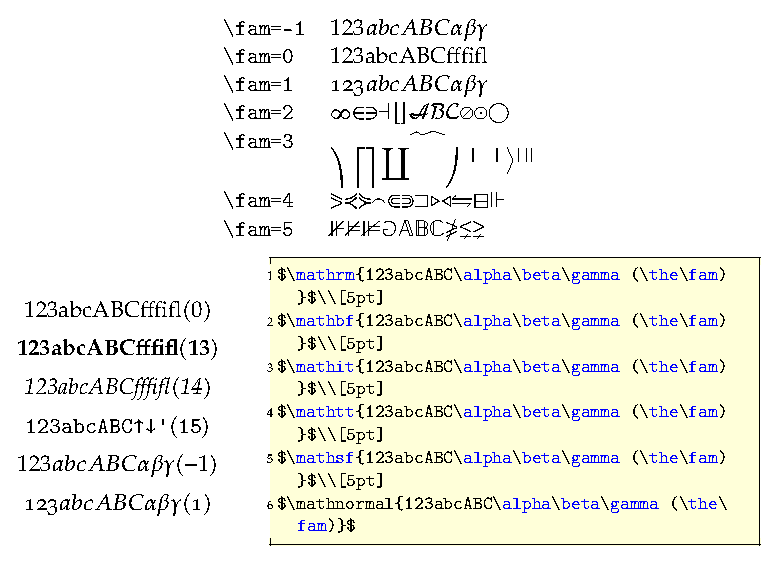
\includegraphics{family}
\iffalse

\begin{center}
\begin{tabular}{ll}
\verb+\fam=-1+ & $\fam=-1 123abcABC\alpha\beta\gamma$\\
\verb+\fam=0+  & $\fam=0 123abcABC\alpha\beta\gamma$\\
\verb+\fam=1+  & $\fam=1 123abcABC\alpha\beta\gamma$\\
\verb+\fam=2+  & $\fam=2 123abcABC\alpha\beta\gamma$\\
\verb+\fam=3+  & $\fam=3 123abcABC\alpha\beta\gamma$\\
\verb+\fam=4+  & $\fam=4 123abcABC\alpha\beta\gamma$\\
\verb+\fam=5+  & $\fam=5 123abcABC\alpha\beta\gamma$
\end{tabular}
\end{center}


\begin{LTXexample}[width=0.3\linewidth]
$\mathrm{123abcABC\alpha\beta\gamma (\the\fam)}$\\[5pt]
$\mathbf{123abcABC\alpha\beta\gamma (\the\fam)}$\\[5pt]
$\mathit{123abcABC\alpha\beta\gamma (\the\fam)}$\\[5pt]
$\mathtt{123abcABC\alpha\beta\gamma (\the\fam)}$\\[5pt]
$\mathsf{123abcABC\alpha\beta\gamma (\the\fam)}$\\[5pt]
$\mathnormal{123abcABC\alpha\beta\gamma (\the\fam)}$
\end{LTXexample}
\fi

\subsection{\CMD{mathaccent}}
\cIndex{mathaccent}Requires three parameter as one number, the class, the font family and the character.

\begin{LTXexample}[width=0.3\linewidth]
\def\dA{\mathaccent"7015\relax}
{\Large $\dA{A}$}
\end{LTXexample}

\subsection{\CMD{mathbin}}
\cIndex{mathbin}Declares a following character as a binary symbol with another 
spacing before and behind such a symbol.

\begin{LTXexample}[width=0.3\linewidth]
{\Large 
$a|b \quad a\mathbin| b$}
\end{LTXexample}

\subsection{\CMD{mathchar}}
\cIndex{mathchar}Declares a math character by three integer numbers as Parameters, giving its class,     %%% ----- Martin -----
font family, and font position. In the following example \verb+\mathchar+ defines a 
character of class 1 (big operators), font family 3 (math extension font) and number
58 (big sum character).

\begin{LTXexample}[width=0.3\linewidth]
{\Large 
$a\sum\limits_{i=1}^{\infty} b \quad 
 a\mathchar"1358\limits_{i=1}^{\infty} b$}
\end{LTXexample}

\subsection{\CMD{mathchardef}}
\cIndex{mathchardef}This is in principle the same as \CIndex{mathchar}, 
it only allows to make such definitions permanent.  

\begin{LTXexample}[width=0.25\linewidth]
\bgroup
\mathchardef\sum="1358
$a\sum\limits_{i=1}^{\infty}\sqrt{i+1}$\\[5pt]
\egroup
 
$a\sum\limits_{i=1}^{\infty}\sqrt{i+1}$ 
\end{LTXexample}


\subsection{\CMD{mathchoice}}
\cIndex{mathchoice}Specifies specific subformula sizes for the 4 main styles: 
\CIndex{displaystyle} -- \CIndex{textstyle} --
\CIndex{scriptstyle} -- \CIndex{scriptscriptstyle}.

\begin{LTXexample}[width=0.15\linewidth]
\Large
\def\myRule{{%
  \color{red}%
  \mathchoice{\rule{2pt}{20pt}}{\rule{1pt}{10pt}}%
    {\rule{0.5pt}{5pt}}{\rule{0.25pt}{2.5pt}}%
    \mkern2mu}}
$\myRule\sum\limits_{\myRule i=1}^{\myRule\infty}%
 \myRule\frac{\myRule\sqrt{\myRule i+1}}{\myRule i^2}$
\end{LTXexample}

\subsection{\CMD{mathclose}}\label{subsec:mathclose}
\cIndex{mathclose}Assigns class 5 (closing character) to the following 
parameter, which can hold a single character or a subformula.

\begin{LTXexample}[width=0.2\linewidth]
{\large
$A:\frac{B}{C}:D$\\[5pt]
$A\mathopen:\frac{B}{C}\mathclose: D $}
\end{LTXexample}


\subsection{\CMD{mathcode}}
\cIndex{mathcode}A math font is far different from a text font. A lot of the characters has to be defined with 
\verb+\mathcode+, which defines the character with its class, font family and character number, \eg
\verb+\mathcode`\<="313C+. It defines the character ``<''{} as a realtion symbol (class 3) from
the font family 1 and the character number 0x3C, which is 60 decimal.

\subsection{\CMD{mathop}}
\cIndex{mathop}Assigns class 1 (large operator) to the parameter, which can be a single character or a subformula.

\begin{LTXexample}[width=0.2\linewidth]
\[ A_{i=1}^{\infty} \]
\[ \mathop{A}_{i=1}^{\infty} \]
\end{LTXexample}

\subsection{\CMD{mathopen}}
\cIndex{mathopen}Vice versa to \verb+\mathclose+ (see section~\ref{subsec:mathclose}).


\subsection{\CMD{mathord}}
\cIndex{mathord}Assigns class 0 (ordinary character) to the following parameter, which can be a single character 
or a subformula.

\begin{LTXexample}[width=0.2\linewidth]
{\large
$y = f(x)$\\[5pt]
$y \mathord= f(x)$}
\end{LTXexample}

\subsection{\CMD{mathpunct}}
\cIndex{mathpunct}Assigns class 6 (punctuation) to the following parameter, which can be a single character
or a subformula (see section~\ref{subsec:dot-comma} for an example).

\subsection{\CMD{mathrel}}
\cIndex{mathrel}Assigns class 3 (relation) to the following parameter, which can be a single character
or a subformula.

\begin{LTXexample}[width=0.25\linewidth]
{\large
$x_1 o x_2 o x_3$\\[5pt]
$x_1\mathrel o x_2\mathrel o x_3$}
\end{LTXexample}


\subsection{\CMD{scriptfont}}
\cIndex{scriptfont}Specifies the scriptstyle font (used for super/subscript) for a family.

\begin{LTXexample}[width=0.25\linewidth]
$A_1$
\font\tenxii=cmr12
\scriptfont0=\tenxii
$A_1$ 
\end{LTXexample}


\subsection{\CMD{scriptscriptfont}}
\cIndex{scriptscriptfont}Specifies the scriptscriptstyle font for a family. 

\subsection{\CMD{scriptscriptstyle}}
\cIndex{scriptscriptstyle}Selects scriptscript style for the following characters.

\subsection{\CMD{scriptstyle}}
\cIndex{scriptstyle}Selects script style for the following characters.


\subsection{\CMD{skew}}
\cIndex{skew}Especially for italic characters double accents are often misplaced. \verb+\skew+ has three arguments
\begin{description}
\item[horizontal shift:] A value in math units for the additional shift of the accent.
\item[the accent:] The symbol which is placed above the character.
\item[the character:] This is in general a single character, but can also include itself an accent.
\end{description}

\AmSmath\ redefines the setting of double accents. This is the reason why there are only a few
cases where someone has to use \verb+\skew+ when the package \PIndex{amsmath} is loaded, like
in this document.

\begin{LTXexample}[width=0.2\linewidth]
\large
$\tilde i$ \qquad $\tilde{A}$\\[5pt]
$\skew{3}{\tilde}{i}$ \qquad $\skew{7}{\tilde}{A}$
\end{LTXexample}

\subsection{\CMD{skewchar}}
\cIndex{skewchar}Is -1 or the character (reference symbol) used to fine-tune the positioning of math accents.

\subsection{\CMD{textfont}}
\cIndex{textfont}Specifies the text font for a family.

\subsection{\CMD{textstyle}}
\cIndex{textstyle}Selects the text style for the following characters.



\section{Math macros}


\subsection{\CMD{above}}
\cIndex{above}
\begin{LTXexample}[width=0.2\linewidth]
$a\above0pt b$\\[8pt]

${a\above1pt b}$\\[8pt]

${a\above2.5pt b}$\\[8pt]

$\displaystyle{a\above0pt b}$
\end{LTXexample}



\subsection{\CMD{abovewithdelims}}
\cIndex{abovewithdelims}
\begin{LTXexample}[width=0.2\linewidth]
$a\abovewithdelims()0pt b$\\[8pt]

\def\fdelimA{\abovewithdelims\{)1.0pt}
${a\fdelimA b}$\\[8pt]

\def\fdelimB{\abovewithdelims[]2.0pt}
${a\fdelimB b}$\\[8pt]

\def\fdelimC{\abovewithdelims\{.0pt}
$\displaystyle{a\fdelimC b}$
\end{LTXexample}

\subsection{\CMD{atop}}
\cIndex{atop}

\begin{LTXexample}[width=0.2\linewidth]
$a\atop b$\\[8pt]

$({n \atop k}) = {n!\above1pt k!(n-k)!}$\\[8pt]

$\displaystyle{a\atop b}$
\end{LTXexample}


\subsection{\CMD{atopwithdelims}}
\cIndex{atopwithdelims}
\begin{LTXexample}[width=0.2\linewidth]
$a\atopwithdelims() b$\\[8pt]

${n \atopwithdelims() k} = {n!\above1pt k!(n-k)!}$\\[8pt]

$\displaystyle{a\atopwithdelims\{. b}$
\end{LTXexample}

\subsection{\CMD{displaylimits}}
\cIndex{displaylimits}Resets the conventions for using limits with operators to the standard for the used environment.

\subsection{\CMD{eqno}}\label{subsec:eqno}
\cIndex{eqno}Puts an equation number at the right margin, the parameter can hold anything. \verb+\eqno+ places
only the parameter, but doesn't increase any equation counter.

\begin{LTXexample}[width=0.5\linewidth]
\[ y=f(x) \eqno{(A12)} \]
\end{LTXexample}

\subsection{\CMD{everydisplay}}
\cIndex{everydisplay}Inserts the parameter at the start of every switch to display math mode.

\begin{LTXexample}[width=0.4\linewidth]
\everydisplay{\color{red}
}
\[ f(x) = \int \frac{\sin x}{x}\,\mathrm{d}x \]
\[ g(x) = \int \frac{\sin^2 x}{x^2}\,\mathrm{d}x \]
\end{LTXexample}

\subsection{\CMD{everymath}}
\cIndex{everymath}Same as \CIndex{everydisplay}, but now for the inline mode. 
In the following example
the displaystyle is used (besides using color red) for every inline math expression.

\bgroup
\begin{LTXexample}[width=0.45\linewidth]
\everymath{\color{red}%
  \displaystyle}
\[ f(x) = \int \frac{\sin x}{x}\,\mathrm{d}x \]
Instead of $\frac{\sin x}{x}$ 
  now with $\frac{\cos x}{x}$:
\[ g(x) = \int \frac{\cos x}{x}\,\mathrm{d}x \]
\end{LTXexample}
\egroup

Pay attention for side effects on footnotes and other macros which use the math mode for superscript
and other math related modes. In this case you'll get the footnotes also in red.

\subsection{\CMD{left}}
\cIndex{left}\TeX{} calculates the size of the following delimiter needed at the left side of a formula.
Requires an additional \verb+right+.

\subsection{\CMD{leqno}}
\cIndex{leqno}Vice versa to \verb+\eqno+ (see section~\vref{subsec:eqno}).

\subsection{\CMD{limits}}
\cIndex{limits}Typesets limits above and/or below operators (see section~\vref{sec:limits}).

\subsection{\CMD{mathinner}}
\cIndex{mathinner}Defines the following parameter as subformula.

\subsection{\CMD{nolimits}}
\cIndex{nolimits}The opposite of \CIndex{limits}, instead of above/below limits are placed to the right of large 
operators (class 1).


\subsection{\CMD{over}}
\cIndex{over}Is equivalent to the fraction macro of \LaTeX{} and equivalent to the 
\verb+\overwithdelims+, see section~\vref{subsec:overwithdelims}.

\begin{LTXexample}[width=0.2\linewidth]
$ {a\over b} \qquad {{m\over n}\over{a+b}} $
\[ {m\over n}\over{a+b} \]
\end{LTXexample}


\subsection{\CMD{overline}}
\cIndex{overline}Puts a line over the following character or subformula and has the same problems with different
heights as underlines (see section~\ref{subsec:underline}).

\begin{LTXexample}[width=0.2\linewidth]
$\overline{x}+\overline{y}=\overline{z}$\\
\let\ol\overline
$ \ol{x} + \ol{A} = \ol{z} $\\[5pt]
\def\yPh{\vphantom{A}}
$ \ol{x\yPh} + \ol{A} = \ol{z\yPh} $
\end{LTXexample}

\subsection{\CMD{overwithdelims}}\label{subsec:overwithdelims}
\cIndex{overwithdelims}Is a generalized fraction command with preset fraction bar thickness.    %%% ----- Martin -----

\begin{LTXexample}[width=0.25\linewidth]
$ {a\overwithdelims() b} \qquad {{m\over n}\overwithdelims[]{a+b}} $
\[ {m\over n}\overwithdelims\{.{a+b} \]
\end{LTXexample}


\subsection{\CMD{radical}}
\cIndex{radical}Makes a radical atom from the delimiter (27-bit number) and the math field.

\begin{LTXexample}[width=0.2\linewidth]
\def\mySqrt{\radical"0270371\relax}
$ \mySqrt{\frac{1}{7}} $\\[5pt]

\def\mySqrt{\radical"0270372\relax}
$ \mySqrt{\frac{1}{7}} $\\[5pt]

\def\mySqrt{\radical"0270373\relax}
$ \mySqrt{\frac{1}{7}} $\\[5pt]

\def\mySqrt{\radical"0270374\relax}
$ \mySqrt{\frac{1}{7}} $\\[5pt]
\end{LTXexample}

\subsection{\CMD{right}}
\cIndex{right}Opposite to \verb+\left+, makes \TeX{} calculate the size of the 
delimiter needed at the right of a formula.

\subsection{\CMD{underline}}\label{subsec:underline}
\cIndex{underline}When there is a combination of variables with and without an index, the underlines are typeset    %%% ----- Martin -----
with a different depth. Using \verb+\vphantom+ in this case is a good choice. 

\begin{LTXexample}[width=0.2\linewidth]
$\underline{x}+\underline{y}=\underline{z}$\\

\let\ul\underline
\def\yPh{\vphantom{y}}
$ \ul{x\yPh} + \ul{y} = \ul{z\yPh} $\\

$ \ul{x_1} + \ul{y_2} = \ul{z_3} $
\end{LTXexample}

\subsection{\CMD{vcenter}}
\cIndex{vcenter}Centers vertical material with respect to the axis.


\section{Math penalties}

\subsection{\CMD{binoppenalty}}
\cIndex{binoppenalty}A penalty for  breaking math expressions between lines in a paragraph. TeX breaks lines only
when the binary symbol is not the last one and when the penalty is below 10,000.

\subsection{\CMD{displaywidowpenalty}}
\cIndex{displaywidowpenalty}The penalty which is added after the penultimate line immediately preceeding a display math formula.

\subsection{\CMD{postdisplaypenalty}}
\cIndex{postdisplaypenalty}Is added immediately after a math display ends.

\subsection{\CMD{predisplaypenalty}}
\cIndex{predisplaypenalty}Is added immediately before a math display starts.

\subsection{\CMD{relpenalty}}
\cIndex{relpenalty}The penalty for a line break after a relation symbol (if a break is possible).


\part{Other packages}
The following sections are not a replacement for the package documentation!
\section{List of available math packages}
\markboth{Math packages}{Math packages}

\begin{center}
\noindent
\begin{tabular}{llll}
\href{http://www.dante.de/CTAN/help/Catalogue/entries/accents.html}{accents}&
\href{http://www.dante.de/CTAN/help/Catalogue/entries/alphalph.html}{alphalph}&
\href{http://www.dante.de/CTAN/help/Catalogue/entries/amsart.html}{amsart}&
\href{http://www.dante.de/CTAN/help/Catalogue/entries/amsbook.html}{amsbook}\\
\href{http://www.dante.de/CTAN//help/Catalogue/entries/amsbsy.html}{amsbsy}&
\href{http://www.dante.de/CTAN//help/Catalogue/entries/amscd.html}{amscd}&
\href{http://www.dante.de/CTAN//help/Catalogue/entries/amscls.html}{amscls}&
\href{http://www.dante.de/CTAN//help/Catalogue/entries/amsfonts.html}{amsfonts}\\
\href{http://www.dante.de/CTAN//help/Catalogue/entries/amslatex.html}{amslatex}&
\href{http://www.dante.de/CTAN//help/Catalogue/entries/amsltx11.html}{amsltx11}&
\href{http://www.dante.de/CTAN//help/Catalogue/entries/amsmath.html}{amsmath}&
\href{http://www.dante.de/CTAN//help/Catalogue/entries/amsppt.html}{amsppt}\\
\href{http://www.dante.de/CTAN//help/Catalogue/entries/amsppt1.html}{amsppt1}&
\href{http://www.dante.de/CTAN//help/Catalogue/entries/amsproc.html}{amsproc}&
\href{http://www.dante.de/CTAN//help/Catalogue/entries/amssym.html}{amssym (plain TeX)}&
\href{http://www.dante.de/CTAN//help/Catalogue/entries/amssymb.html}{amssymb (LaTeX)}\\
\href{http://www.dante.de/CTAN//help/Catalogue/entries/amstex.html}{amstex (Plain TeX)}&
\href{http://www.dante.de/CTAN//help/Catalogue/entries/amstext.html}{amstext}&
\href{http://www.dante.de/CTAN//help/Catalogue/entries/amsthm.html}{amsthm}&
\href{http://www.dante.de/CTAN//help/Catalogue/entries/bez123.html}{bez123}\\
\href{http://www.dante.de/CTAN//help/Catalogue/entries/bitfield.html}{bitfield}&
\href{http://www.dante.de/CTAN//help/Catalogue/entries/brclc.html}{brclc}&
\href{http://www.dante.de/CTAN//help/Catalogue/entries/breqn.html}{breqn}&
\href{http://www.dante.de/CTAN//help/Catalogue/entries/cancel.html}{cancel}\\
\href{http://www.dante.de/CTAN//help/Catalogue/entries/cases.html}{cases}&
\href{http://www.dante.de/CTAN//help/Catalogue/entries/comma.html}{comma}&
\href{http://www.dante.de/CTAN//help/Catalogue/entries/datenumber.html}{datenumber}&
\href{http://www.dante.de/CTAN//help/Catalogue/entries/diagxy.html}{diagxy}\\
\href{http://www.dante.de/CTAN//help/Catalogue/entries/doublestroke.html}{doublestroke}&
\href{http://www.dante.de/CTAN//help/Catalogue/entries/easyeqn.html}{easyeqn}&
\href{http://www.dante.de/CTAN//help/Catalogue/entries/easybmat.html}{easybmat}&
\href{http://www.dante.de/CTAN//help/Catalogue/entries/easymat.html}{easymat}\\
\href{http://www.dante.de/CTAN//help/Catalogue/entries/eqnarray.html}{eqnarray}&
\href{http://www.dante.de/CTAN//help/Catalogue/entries/esvect.html}{esvect}&
\href{http://www.dante.de/CTAN//help/Catalogue/entries/fixmath.html}{fixmath}&
\href{http://www.dante.de/CTAN//help/Catalogue/entries/fltpoint.html}{ftlpoint}\\
\href{http://www.dante.de/CTAN//help/Catalogue/entries/icomma.html}{icomma}&
\href{http://www.dante.de/CTAN//help/Catalogue/entries/leftidx.html}{leftidx}&
\href{http://www.dante.de/CTAN//help/Catalogue/entries/mathdots.html}{mathdots}&
\href{http://www.dante.de/CTAN//help/Catalogue/entries/mathtools.html}{mathtools}\\
\href{http://www.dante.de/CTAN//help/Catalogue/entries/mathematica.html}{mathematica}&
\href{http://www.dante.de/CTAN//help/Catalogue/entries/mil3.html}{mil3}&
\href{http://www.dante.de/CTAN//help/Catalogue/entries/mtbe.html}{mtbe}&
\href{http://www.dante.de/CTAN//help/Catalogue/entries/nath.html}{Nath}\\
\href{http://www.dante.de/CTAN//help/Catalogue/entries/numprint.html}{numprint}&
\href{http://www.dante.de/CTAN//help/Catalogue/entries/random.html}{random}&
\href{http://www.dante.de/CTAN//help/Catalogue/entries/romannum.html}{romannum}&
\href{http://www.dante.de/CTAN//help/Catalogue/entries/texaide.html}{TeXaide}
\end{tabular}
\end{center}

The following examples depend on the listed versions of the packages:    %%% ----- Martin -----

{\small
\begin{verbatim}
  amsopn.sty    1999/12/14 v2.01 operator names
      bm.sty    1999/07/05 v1.0g Bold Symbol Support (DPC/FMi)
  empheq.sty    2007/12/03 v2.12 Emphasizing equations (MH)
   amscd.sty    1999/11/29 v2.0
 accents.sty    2000/08/06 v1.2 Math Accent Tools
  framed.sty    2007/10/04 v 0.95: framed or shaded text with page breaks
pstricks.sty    2004/05/06 v0.2k LaTeX wrapper for `PSTricks' (RN,HV)
pstricks.tex    2003/03/07 v97 patch 15 `PSTricks' (tvz)
pst-node.tex    2008/11/26 v1.01 PSTricks package for nodes (tvz,hv)
delarray.sty    1994/03/14 v1.01 array delimiter package (DPC)
   xypic.sty    1999/02/16 Xy-pic version 3.7
 exscale.eps    Graphic file (type veps)
\end{verbatim}
}


\subsection{\texttt{accents}}\label{sec:package-accent}
If you want to write for example an underlined M, then you can do it by    %%% ----- Martin -----

\medskip
\begin{tabular}{ll}
\verb|\underline{$M$}| & \underline{$M$}\\
\verb|\underbar{$M$}|  & \underbar{$M$}\\
\verb|\underaccent{\bar}{M}| & $\underaccent{\bar}{M}$
\end{tabular}
\medskip

As seen, there is no difference between \CMD{underline} and \CMD{underbar}. For    %%% ----- Martin -----
some reasons it may be better to use the \PIndex{accent} package with the
\CMD{underaccents} macro.

\subsection{\texttt{amscd} -- commutative diagrams}

The \PIndex{amscd} package is part of the \AmSmath bundle
or available at CTAN%
\footnote{\href{http://www.ctan.org/tex-archive/macros/latex/required/amslatex/math/amscd.dtx}%
{CTAN://macros/latex/required/amslatex/math/amscd.dtx}} and has no options for the
\verb|\usepackage| command.
\texttt{amscd} does not support diagonal arrows but is much     %%% ----- Martin -----
easier to handle than the complex \PIndex{pstricks} package or
the \PIndex{xypic} package. On the other hand simple diagrams
can be written with the \UIndex{array} or look at \cite{taylor00}.

\[
\begin{CD}
  R\times S\times T @>\text{restriction}>> S\times T \\
        @VprojVV                            @VVprojV \\
  R\times S         @<<\text{inclusion}<        S
\end{CD}
\]

\begin{lstlisting}
\[
\begin{CD}
  R\times S\times T @>\text{restriction}>> S\times T \\
        @VprojVV                            @VVprojV \\
  R\times S         @<<\text{inclusion}<        S
\end{CD}
\]
\end{lstlisting}


\subsection{\texttt{amsopn}}\label{sec:amsopn}
With the \PIndex{amsopn} package it is very easy to declare new math operators, which are written in
upright mode:

$\underset{s=p}{Res}\quad\text{versus}\quad\underset{s=p}{\Res}$

\medskip
\begin{lstlisting}
\documentclass[10pt]{article}
\usepackage{amsmath}
\usepackage{amsopn}
\DeclareMathOperator{\Res}{Res}
\begin{document}
$\underset{s=p}{Res}\quad\underset{s=p}{\Res}$
\end{document}
\end{lstlisting}

Table~\ref{tab:amsopn} shows the predefined operatornames of \verb+amsopn+.

\begin{table}[htb]
\centering
\begin{tabular}{llllll}
\verb+\arccos+ & $\arccos$ & \verb+\arcsin+ & $\arcsin$ & \verb+\arctan+ & $\arctan$\\
\verb+\arg+    & $\arg$    & \verb+\cos+    & $\cos$    & \verb+\cosh+   & $\cosh$\\
\verb+\cot+    & $\cot$    & \verb+\coth+   & $\coth$   & \verb+\csc+    & $\csc$\\
\verb+\deg+    & $\deg$    & \verb+\det+    & $\det$    & \verb+\dim+    & $\dim$\\
\verb+\exp+    & $\exp$    & \verb+\gcd+    & $\gcd$    & \verb+\hom+    & $\hom$\\
\verb+\inf+    & $\inf$    & \verb+\injlim+ & $\injlim$ & \verb+\ker+    & $\ker$\\
\verb+\lg+     & $\lg$     & \verb+\lim+    & $\lim$    & \verb+\liminf+ & $\liminf$\\
\verb+\limsup+ & $\limsup$ & \verb+\ln+     & $\ln$     & \verb+\log+    & $\log$\\
\verb+\max+    & $\max$    & \verb+\min+    & $\min$    & \verb+\Pr+     & $\Pr$\\
\verb+\projlim+& $\projlim$& \verb+\sec+    & $\sec$    & \verb+\sin+    & $\sin$\\
\verb+\sinh+   & $\sinh$   & \verb+\sup+    & $\sup$    & \verb+\tan+    & $\tan$\\
\verb+\tanh+   & $\tanh$
\end{tabular}
\caption{The predefined operators of \texttt{amsopn.sty}}\label{tab:amsopn}
\end{table}


\subsection{\texttt{bigdel}}\label{sec:bigdelim}
This is a very useful package together with the \PIndex{multirow} package.
In the following example we need additional parentheses for a different
number of rows. This is also possible with the \UIndex{array},
but not as easy as with the \PIndex{bigdelim} package. The trick is that you need one
separate column for a big delimiter, but with empty cells in all rows, which
the delimiter spans. 

\[
  \begin{pmatrix}
     & x_{11} & x_{12} & \dots & x_{1p} & \rdelim\}{4}{3cm}[some text]\\
     \ldelim[{5}{1cm}[text] & x_{21} & x_{22} & \dots & x_{2p} \\
     & \vdots\\
     & x_{n_1 1}& x_{n_1 2} & \dots & x_{n_1 p}\\
     & x_{n_1+1,1}&x_{n_1+1,2} & \dots & x_{n_1+1, p} &
         \rdelim\}{3}{3cm}[some more text]\\
     & \vdots\\
     & x_{n_1+n_2, 1} & x_{n_1+n_2,2} & \dots & x_{n_1+n_2,p}\\
     & \vdots \\
  \end{pmatrix}
\]

\begin{lstlisting}[xleftmargin=-1cm,xrightmargin=-1.5cm]
\[
  \begin{pmatrix}
     & x_{11} & x_{12} & \dots & x_{1p} & \rdelim\}{4}{3cm}[some text]\\
     \ldelim[{5}{1cm}[text] & x_{21} & x_{22} & \dots & x_{2p} \\
     & \vdots\\
     & x_{n_1 1}& x_{n_1 2} & \dots & x_{n_1 p}\\
     & x_{n_1+1,1}&x_{n_1+1,2} & \dots & x_{n_1+1, p} &
         \rdelim\}{3}{3cm}[some more text]\\
     & \vdots\\
     & x_{n_1+n_2, 1} & x_{n_1+n_2,2} & \dots & x_{n_1+n_2,p}\\
     & \vdots \\
  \end{pmatrix}
\]
\end{lstlisting}

As seen in the above listing the left big delimiter is placed in the first
column, all other rows start with second column. It is possible to use all
columns above and below the delimiter. For the \UIndex{array}
there must be two more columns defined, in case of a big delimiter left and
right. The syntax of \CIndex{ldelim} and \CIndex{rdelim} is:
%
\begin{verbatim}
\ldelim<delimiter>{<n rows>}{<added horizontal space>}[<text>]
\rdelim<delimiter>{<n rows>}{<added horizontal space>}[<text>]
\end{verbatim}

Any delimiter which is possible for the \CIndex{left} or \CIndex{right} command
is allowed, \eg ``\verb/()[]{}|/''. The text is an optional argument and 
always typeset in text mode.

\subsection{\texttt{bm}}\label{sec:bm}
By default the math macro \CIndex{mathbf} writes everything in bold and in upright mode
$\mathbf{y=f(x)}$  (\verb|$\mathbf{y=f(x)}$|), but it should be in italic mode especially
for variables $\bm{y=f(x)}$ (\verb|$\bm{y=f(x)}$|), which is possible with the package \PIndex{bm}. 
For writing a whole formula in bold have a look at section~\vref{sec:boldmath}.


\subsection{\texttt{braket}}\label{sec:braket}
It is available at
 \href{http://www.ctan.org/tex-archive/macros/latex/contrib/other/misc/braket.sty}%
{CTAN://macros/latex/contrib/other/misc/braket.sty}
and provides several styles for writing math expressions inside brakets. For example:

\[ \left\{ x\in\mathbf{R} | 0<{|x|}<\frac{5}{3}\right\} \]

\begin{lstlisting}
\[ \left\{ x\in\mathbf{R} | 0<{|x|}<\frac{5}{3}\right\} \]
\end{lstlisting}

\noindent looks not quite right and it is not really easy to get the first vertical line in the same
size as the outer braces. Some solution may be using \CIndex{vphantom}:

\[
\left\{\vphantom{\frac{5}{3}}x\in\mathbf{R} \right|\left. 0<{|x|}<\frac{5}{3}\right\}
\]

\begin{lstlisting}
\[
\left\{\vphantom{\frac{5}{3}}x\in\mathbf{R} \right|\left. 0<{|x|}<\frac{5}{3}\right\}
\]
\end{lstlisting}

The package \PIndex{braket} has the macros

\begin{lstlisting}
\Bra{<math expression>}
\Ket{<math expression>}
\Braket{<math expression>}
\Set{<math expression>}
\end{lstlisting}

\noindent and the same with a leading lower letter, which are not really interesting.

\[ \Bra{x\in\mathbf{R} | 0<|x|<\frac{5}{3}} \]
\[ \Ket{x\in\mathbf{R} | 0<|x|<\frac{5}{3}} \]
\[ \Braket{x\in\mathbf{R} | 0<|x|<\frac{5}{3}} \]
\[ \Braket{x\in\mathbf{R} | 0<\vert x\vert <\frac{5}{3}} \]
\[ \Set{x\in\mathbf{R} | 0<|x|<\frac{5}{3}} \]

\begin{lstlisting}
\[ \Bra{x\in\mathbf{R} | 0<|x|<\frac{5}{3}} \]
\[ \Ket{x\in\mathbf{R} | 0<|x|<\frac{5}{3}} \]
\[ \Braket{x\in\mathbf{R} | 0<|x|<\frac{5}{3}} \]
\[ \Braket{x\in\mathbf{R} | 0<\vert x\vert <\frac{5}{3}} \]
\[ \Set{x\in\mathbf{R} | 0<|x|<\frac{5}{3}} \]
\end{lstlisting}

The difference between the \CIndex{Set} and the \CIndex{Braket} macro is the  handling of the
vertical lines. In \CIndex{Set} only the first one gets the same size as the
braces\index{Braces} and in \CIndex{Braket} all.

\[  \Braket{ \phi | \frac{\partial^2}{\partial t^2} | \psi }\]
\[  \Set{ \phi | \frac{\partial^2}{\partial t^2} | \psi }\]
\begin{lstlisting}
\[\Braket{\phi | \frac{\partial^2}{\partial t^2} | \psi}\]
\[\Set{\phi | \frac{\partial^2}{\partial t^2} | \psi}\]
\end{lstlisting}


\CMD{Bra} and \CMD{Ket} do nothing with the inner vertical lines.


\subsection{\texttt{cancel}}\label{cancel.sty}
This is a nice package for canceling anything in mathmode with a slash, 
backslash or a \verb+X+. To get
a horizontal line we can define an additional macro called \CIndex{hcancel} 
with an optional argument
for the line color (requires package \PIndex{color}):
%
\begin{lstlisting}
\newcommand\hcancel[2][black]{\setbox0=\hbox{#2}%
	\rlap{\raisebox{.45\ht0}{\textcolor{#1}{\rule{\wd0}{1pt}}}}#2}
\end{lstlisting}

It is no problem to redefine the \CIndex{cancel} macros to get also colored lines. 
A horizontal line for
single characters is also decribed in section~\vref{sec:Accents}.

\medskip
\noindent
\verb+\cancel+: $f(x)=\dfrac{\left(x^2+1\right)\cancel{(x-1)}}{\cancel{(x-1)}(x+1)}$\\[0.5cm]
\verb+\bcancel+: $\bcancel{3}\qquad\bcancel{1234567}$\\[0.5cm]
\verb+\xcancel+: $\xcancel{3}\qquad\xcancel{1234567}$\\[0.5cm]
\verb+\hcancel+: $\hcancel{3}\qquad\hcancel[red]{1234567}$

\bigskip
\begin{lstlisting}
$f(x)=\dfrac{\left(x^2+1\right)\cancel{(x-1)}}{\cancel{(x-1)}(x+1)}$\\[0.5cm]
$\bcancel{3}\qquad\bcancel{1234567}$\\[0.5cm]
$\xcancel{3}\qquad\xcancel{1234567}$\\[0.5cm]
$\hcancel{3}\qquad\hcancel[red]{1234567}$
\end{lstlisting}


\subsection{\texttt{cool}}\label{cool}
The \PIndex{cool} package defines a lot of special mathematical expressions 
to use them by the macro name. The following list shows only some of
them, for more informations look at the example file, which comes with
the package.  

\bgroup
\parindent=0pt
\bigskip
\begin{tabular}{@{}ll@{}}
\CIndex{Sin}\verb|{x}|	& $\displaystyle \Sin{x}$\\
\CIndex{Cos}\verb|{x}|	& $\displaystyle \Cos{x}$\\
\CIndex{Tan}\verb|{x}|	& $\displaystyle \Tan{x}$\\
\CIndex{Csc}\verb|{x}|	& $\displaystyle \Csc{x}$\\
\CIndex{Sec}\verb|{x}|	& $\displaystyle \Sec{x}$\\
\CIndex{Cot}\verb|{x}|	& $\displaystyle \Cot{x}$
\end{tabular}

\bigskip
\Style{ArcTrig=inverse}%
\CMD{Style\{ArcTrig=inverse\}} (default)

\bigskip
\begin{tabular}{@{}ll@{}}
\CIndex{ArcSin}\verb|{x}|& $\displaystyle \ArcSin{x}$\\
\CIndex{ArcCos}\verb|{x}|& $\displaystyle \ArcCos{x}$\\
\CIndex{ArcTan}\verb|{x}|& $\displaystyle \ArcTan{x}$
\end{tabular}

\bigskip
\Style{ArcTrig=arc}
\CMD{Style\{ArcTrig=arc\}}

\bigskip
\begin{tabular}{@{}ll@{}}
\CIndex{ArcSin}\verb|{x}| & $\displaystyle \ArcSin{x}$\\
\CIndex{ArcCos}\verb|{x}| & $\displaystyle \ArcCos{x}$\\
\CIndex{ArcTan}\verb|{x}| & $\displaystyle \ArcTan{x}$\\
\CIndex{ArcCsc}\verb|{x}| & $\displaystyle \ArcCsc{x}$\\
\CIndex{ArcSec}\verb|{x}| & $\displaystyle \ArcSec{x}$\\
\CIndex{ArcCot}\verb|{x}| & $\displaystyle \ArcCot{x}$
\end{tabular}


\bigskip
\begin{tabular}{@{}ll@{}}
\CIndex{Factorial}\verb|{n}|	& $\displaystyle \Factorial{n}$\\
\CIndex{DblFactorial}\verb|{n}|	& $\displaystyle \DblFactorial{n}$\\
\CIndex{Binomial}\verb|{n}{k}|	& $\displaystyle \Binomial{n}{k}$\\
\CIndex{Multinomial}\verb|{1,2,3,4}|& $\displaystyle \Multinomial{i_1,\ldots,i_n}$
\end{tabular}

\bigskip
\begin{tabular}{@{}ll@{}}
\CIndex{GammaFunc}\verb|{x}|	& $\displaystyle \GammaFunc{x}$\\
\CIndex{IncGamma}\verb|{a}{x}|	& $\displaystyle \IncGamma{a}{x}$\\
\CIndex{GenIncGamma}\verb|{a}{x}{y}|& $\displaystyle \GenIncGamma{a}{x}{y}$	\\
\CIndex{RegIncGamma}\verb|{a}{x}|& $\displaystyle \RegIncGamma{a}{x}$	\\
\CIndex{RegIncGammaInv}\verb|{a}{x}|& $\displaystyle \RegIncGammaInv{a}{x}$	\\
\CIndex{GenRegIncGamma}\verb|{a}{x}{y}|	& $\displaystyle \GenRegIncGamma{a}{x}{y}$\\
\CIndex{GenRegIncGammaInv}\verb|{a}{x}{y}|& $\displaystyle \GenRegIncGammaInv{a}{x}{y}$\\
\CIndex{Pochhammer}\verb|{a}{n}|	& $\displaystyle \Pochhammer{a}{n}$	\\
\CIndex{LogGamma}\verb|{x}|		& $\displaystyle \LogGamma{x}$
\end{tabular}


\bigskip

\begin{tabular}{@{}ll@{}}
\CIndex{Hypergeometric}\verb|{0}{0}{}{}{x}| & $\displaystyle \Hypergeometric{0}{0}{}{}{x}$\\
\CIndex{Hypergeometric}\verb|{0}{1}{}{b}{x}|& $\displaystyle \Hypergeometric{0}{1}{}{b}{x}$
\end{tabular}


\bigskip
\begin{tabular}{@{}ll@{}}
\CIndex{RegHypergeometric}\verb|{0}{0}{}{}{x}| & $\displaystyle \RegHypergeometric{0}{0}{}{}{x}$\\
\CIndex{RegHypergeometric}\verb|{0}{1}{}{b}{x}|& $\displaystyle \RegHypergeometric{0}{1}{}{b}{x}$
\end{tabular}



\bigskip
\begin{tabular}{@{}l@{}}
\CIndex{MeijerG}\verb|[a,b]{n}{p}{m}{q}{x}| \\
 \hspace*{2cm} $\displaystyle \MeijerG[a,b]{n}{p}{m}{q}{x}$ \\
\CIndex{MeijerG}\verb|{1,2,3,4}{5,6}{3,6,9}{12,15,18,21,24}{x}| \\
 \hspace*{2cm} $\displaystyle \MeijerG{1,2,3,4}{5,6}{3,6,9}{12,15,18,21,24}{x}$
\end{tabular}

\index{Zeta!Functions}
\index{Polylogarithm}
\index{Zeta!Riemann}
\index{Zeta!Hurwitz}
\index{Zeta}

\bigskip
\begin{tabular}{@{}ll@{}}
\CIndex{RiemannZeta}\verb|{s}|	& $\displaystyle \RiemannZeta{s}$\\
\CIndex{Zeta}\verb|{s}|		& $\displaystyle \Zeta{s}$\\
\CIndex{HurwitzZeta}\verb|{s}{a}|& $\displaystyle \HurwitzZeta{s}{a}$\\
\CIndex{Zeta}\verb|{s,a}|	 & $\displaystyle \Zeta{s,a}$	\\
\CIndex{RiemannSiegelTheta}\verb|{x}|& $\displaystyle \RiemannSiegelTheta{x}$	\\
\CIndex{RiemannSiegelZ}\verb|{x}|	& $\displaystyle \RiemannSiegelZ{x}$		\\
\CIndex{StieltjesGamma}\verb|{n}|	& $\displaystyle \StieltjesGamma{n}$
\end{tabular}


\index{Mathieu!Functions}
\index{Mathieu!Characteristics}

\bigskip
\begin{tabular}{@{}ll@{}}
\CIndex{MathieuC}\verb|{a}{q}{z}|	& $\displaystyle \MathieuC{a}{q}{z}$	\\
\CIndex{MathieuS}\verb|{a}{q}{z}| 	& $\displaystyle \MathieuS{a}{q}{z}$
\end{tabular}


\bigskip
\begin{tabular}{@{}ll@{}}
\CIndex{MathieuCharacteristicA}\verb|{r}{q}|& $\displaystyle \MathieuCharacteristicA{r}{q}$	\\
\CIndex{MathieuCharisticA}\verb|{r}{q}|	& $\displaystyle \MathieuCharisticA{r}{q}$	\\

%%%%%%% Characteristic Value of Even Mathieu Fucntion b_r(q)
\CIndex{MathieuCharacteristicB}\verb|{r}{q}|& $\displaystyle \MathieuCharacteristicB{r}{q}$	\\
\CIndex{MathieuCharisticB}\verb|{r}{q}|& $\displaystyle \MathieuCharisticB{r}{q}$	\\
				
%%%%%%%% Characteristic Exponent of a Mathieu Fucntion r(a,q)
\CIndex{MathieuCharacteristicExponent}\verb|{a}{q}|& $\displaystyle \MathieuCharacteristicExponent{a}{q}$\\
\CIndex{MathieuCharisticExp}\verb|{a}{q}|& $\displaystyle \MathieuCharisticExp{a}{q}$
\end{tabular}
\egroup

\subsection{\texttt{delarray}}\label{delarray}

Package \PIndex{delarray}%
\footnote{\href{http://www.ctan.org/tex-archive/macros/latex/required/tools/delarray.dtx}{CTAN://macros/latex/required/tools/delarray.dtx}%
} supports different delimiters which are defined together with the
beginning of an array:

\begin{lstlisting}
\begin{array}<delLeft>{cc}<delRight>
...
\end{lstlisting}

\noindent defines an array with two centered columns and the delimiters\\
``\texttt{<delLeft><delRight>}{}'', \eg ``\texttt{()}{}''.

\medskip{}
\begin{minipage}[c]{0.45\textwidth}%
\begin{lstlisting}
\[
A=\begin{array}({cc})
	a & b\\
	c & d
\end{array}
\]
\end{lstlisting}

\end{minipage}%
\hfill{}\begin{minipage}[c]{0.45\textwidth}%
\[
A=\begin{array}({cc})
a & b \\
c & d
\end{array}
\]
\end{minipage}%

\medskip{}

The \PIndex{delarray} package expects a pair of delimiters. If you need only
one (like the cases structure) then use the dot for an ``empty''
delimiter, \eg

\medskip{}
\begin{minipage}[c]{0.45\textwidth}%
\begin{lstlisting}
\[
A=\begin{array}\{{cc}.
	a & b\\
	c & d
\end{array}
\]
\end{lstlisting}

\end{minipage}%
\hfill{}\begin{minipage}[c]{0.45\textwidth}%
\[A=\begin{array}\{{cc}.
a & b \\
c & d
\end{array}\]
\end{minipage}%

\medskip{}

\noindent which is a useful command for a cases structure without the \AmSmath 
package, which is described in the \AmSmath part.


\subsection{\texttt{dotseqn}}\label{dotseqn}
This package%
\footnote{\href{http://www.ctan.org/tex-archive/macros/latex/contrib/dotseqn/}%
{CTAN://macros/latex/contrib/dotseqn}} fills the space between the math 
expression and the equation
number with dots. Expect problems when using this package together with \AmSmath.

\begingroup
\makeatletter 
% package couldn't be loaded, it redefines the math
% environments
\newcommand\EqnDots{\leaders\hbox{\kern4\p@ .\kern4\p@}\hfill}
\@ifundefined{mathindent}{\newdimen\mathindent \mathindent\leftmargini}{}
\renewcommand{\[}{\relax \ifmmode\@badmath \else
 \begin{trivlist}%
  \@beginparpenalty\predisplaypenalty \@endparpenalty\postdisplaypenalty
  \item[]\leavevmode \hbox to\linewidth\bgroup $\m@th\displaystyle %$
  \hskip\mathindent\bgroup
 \fi}
\renewcommand{\]}{\relax\ifmmode \egroup $\hfil% $
    \egroup \end{trivlist}%
  \else \@badmath \fi}
\renewenvironment{equation}%
 {\@beginparpenalty\predisplaypenalty \@endparpenalty\postdisplaypenalty
     \refstepcounter{equation}\trivlist \item[]\leavevmode
       \hbox to\linewidth\bgroup $\m@th% $
         \displaystyle \hskip\mathindent}%
 {$\EqnDots % $   Replace `\hfil' with dotted leaders `\EqnDots'.
     \displaywidth\linewidth\hbox{\@eqnnum}\egroup \endtrivlist}
\renewenvironment{eqnarray}{%
   \stepcounter{equation}%
   \def\@currentlabel{\p@equation\theequation}%
   \global\@eqnswtrue \m@th \global\@eqcnt\z@  \tabskip\mathindent
   \let\\\@eqncr \setlength\abovedisplayskip\topsep
   \ifvmode \addtolength\abovedisplayskip\partopsep \fi
   \addtolength\abovedisplayskip\parskip
   \setlength\belowdisplayskip\abovedisplayskip
   \setlength\belowdisplayshortskip\abovedisplayskip
   \setlength\abovedisplayshortskip\abovedisplayskip
   $$\everycr{}\halign to\linewidth% $$
   \bgroup
     \hskip\@centering
     $\displaystyle\tabskip\z@skip{##}$\@eqnsel&%
     \global\@eqcnt\@ne \hfil${\DEQ@acs##\DEQ@acs}$\hfil&%
     \global\@eqcnt\tw@ $\displaystyle{##}$\hskip\@centering\cr%
 }% end of "\begin" part
 {\@@eqncr
   \noalign{% vertical skip up to overlay phantom line
      \penalty\@M \vskip-\prevdepth
      \edef\@tempa{\omit\span\omit\span\omit   % span three columns
        \vrule\@depth\the\prevdepth \@width\z@ % strut of proper depth
        \kern-\mathindent \kern\linewidth}%    % full line width
      \nointerlineskip \expandafter % use saved |\@tempa| outside group
   }\@tempa\cr
   \egroup
   \global\advance\c@equation\m@ne$$% $$
   \global\@ignoretrue
 }
\def\@@eqncr{\let\reserved@a\@empty
   \ifcase\@eqcnt \def\reserved@a{& &}\or \def\reserved@a{&}\fi
   \reserved@a
   \if@eqnsw \egroup $\EqnDots \@eqnnum $\bgroup \stepcounter{equation}%
   \fi \global\@eqnswtrue\global\@eqcnt\z@\cr}
\def\DEQ@acs{\hskip\tw@\arraycolsep}
\makeatother
\begin{eqnarray} 
  F(x) &=& \int f(x)\,\mathrm{d}x + C 
\end{eqnarray}
%
\begin{equation}
  F(x)=\int f(x)\,\mathrm{d}x + C 
\end{equation}
\endgroup

\begin{lstlisting}
\begin{eqnarray} 
  F(x) &=& \int f(x)\,\mathrm{d}x + C 
\end{eqnarray}
%
\begin{equation}
  F(x)=\int f(x)\,\mathrm{d}x + C 
\end{equation}
\end{lstlisting}


\subsection{\texttt{empheq}}\label{sec:empheq}

This package\footnote{The package is part of the \texttt{mh}-bundle 
of Morten H\o gholm (\href{http://www.ctan.org/tex-archive/macros/latex/contrib/mh/}{CTAN://macros/latex/contrib/mh/}).} 
supports different frames for math environments of the \AmSmath
package. It doesn't support  all the environments from standard \LaTeX{} which 
are not modified by \AmSmath, \eg \UIndex{eqnarray}.

With the optional argument of the \UIndex{empheq} 
the preferred box type
can be specified. A simple one is \CIndex{fbox}

\begin{empheq}[box=\fbox]{align}
	f(x)=\int_1^{\infty}\frac{1}{x^2}\,\mathrm{d}x=1
\end{empheq}

\begin{lstlisting}
\begin{empheq}[box=\fbox]{align}
	f(x)=\int_1^{\infty}\frac{1}{x^2}\,\mathrm{d}x=1
\end{empheq}
\end{lstlisting}

The same is possible with the macro \verb|\colorbox|:
\begin{empheq}[box={\fboxsep=10pt\colorbox{yellow}}]{align}
	f(x)=\int_1^{\infty}\frac{1}{x^2}\,\mathrm{d}x=1
\end{empheq}

\begin{lstlisting}
\begin{empheq}[box={\fboxsep=10pt\colorbox{yellow}}]{align}
	f(x)=\int_1^{\infty}\frac{1}{x^2}\,\mathrm{d}x=1
\end{empheq}
\end{lstlisting}

The key \verb|box| can hold any possible \LaTeX{} command sequence. Boxing
subequations is also no problem, the \UIndex{empheq} works in the same way:

\begin{subequations}
\begin{empheq}[box={\fboxsep=10pt\colorbox{cyan}}]{align}
	f(x) & =\int_1^{\infty}\frac{1}{x^1}\,\mathrm{d}x=1\\
	f(x) & =\int_2^{\infty}\frac{1}{x^2}\,\mathrm{d}x=0.25
\end{empheq}
\end{subequations}

\begin{lstlisting}
\begin{subequations}
\begin{empheq}[box={\fboxsep=10pt\colorbox{cyan}}]{align}
	f(x) & =\int_1^{\infty}\frac{1}{x^2}\,\mathrm{d}x=1\\
	f(x) & =\int_2^{\infty}\frac{1}{x^2}\,\mathrm{d}x=0.25
\end{empheq}
\end{subequations}
\end{lstlisting}

For more information on \PIndex{empheq} package have a look at the documentation of the package
which is available at any CTAN server.

\subsection{\texttt{esint}}\label{sec:esint}
This is a very useful package when you want nice double or triple integral or curve
integral symbols. The ones from the \PIndex{wasysym} package%
\footnote{\href{http://www.ctan.org/tex-archive/macros/latex/contrib/wasysym/}%
{CTAN://macros/latex/contrib/wasysym/}} are not the best.
\verb|esint|\footnote{\href{http://www.ctan.org/tex-archive/macros/latex/contrib/esint/}%
{CTAN://macros/latex/contrib/esint/}
\href{http://www.ctan.org/tex-archive/fonts/ps-type1/esint/}{CTAN://fonts/ps-type1/esint/}} supports the following symbols:

\allowdisplaybreaks
\begin{align}
\text{\CMD{int}}      &: \int\\
\text{\CMD{iint}}     &: \iint\\
\text{\CMD{iiintop}}  &: \iiintop\\
\text{\CMD{iiiintop}} &: \iiiintop\\
\text{\CMD{dotsintop}}&: \dotsintop\\
\text{\CMD{ointop}}   &: \ointop\\
\text{\CMD{oiint}}    &: \oiint\\
\text{\CMD{sqint}}    &: \sqint\\
\text{\CMD{sqiint}}   &: \sqiint\\
\text{\CMD{ointctrclockwise}}    &: \ointctrclockwise\\
\text{\CMD{ointclockwise}}       &: \ointclockwise\\
\text{\CMD{varointclockwise}}    &: \varointclockwise\\
\text{\CMD{varointctrclockwise}} &: \varointctrclockwise\\
\text{\CMD{fint}}        &: \fint\\
\text{\CMD{varoiint}}    &: \varoiint\\
\text{\CMD{landupint}}   &: \landupint\\
\text{\CMD{landdownint}} &: \landdownint
\end{align}


\subsection{\texttt{eucal} and \texttt{euscript}}\label{sec:euscript.sty}

These packages should be part of your local \TeX{} installation, because
they come with the \AmSmath packages. Otherwise get them from CTAN%
\footnote{\href{http://www.ctan.org/tex-archive/fonts/amsfonts/latex/euscript.sty}%
{CTAN://fonts/amsfonts/latex/euscript.sty}}. They support a scriptwriting of only uppercase
letters:

\begin{center}
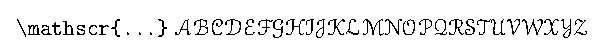
\includegraphics{EuScript}
%\texttt{\textbackslash{}mathscr\{...\}}\index{EuScript@\textbackslash EuScript}
%{$\EuScript{ABCDEFGHIJKLMNOPQRSTUVWXYZ}$}
\end{center}

Read the documentation for the interdependence to the    %%% ----- Martin -----
\verb|\mathcal| command. For the above example the
package \PIndex{eucal} was loaded with the option \verb|mathscr|.


\subsection{\texttt{exscale}}\label{sec:exscale}

The following formula is written with the default fontsize where everything
looks more or less well:

\[
\int_{-1}^{+1}\frac{f(x)}{\sqrt{1-x^{2}}}\,%
\,\mathrm{d}x\approx\frac{\pi}{n}\sum_{i=1}^{n}f\left(\cos\left(\frac{2i-1}{2n}\right)\right)\]


Writing the same with the fontsize \CIndex{huge} gives
a surprising result, which belongs to the historical development of
\LaTeX{}, the \CIndex{int} and \CIndex{sum} symbols
are not stretched. This extreme fontsize is often needed for slides
and not only written ``just for fun{}''.

\begin{center}
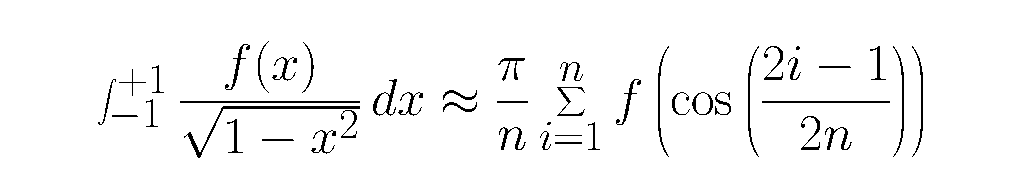
\includegraphics{exscale}
\end{center}

Using the \PIndex{exscale} package%
\footnote{\href{http://www.ctan.org/tex-archive/macros/latex/base/}%
{CTAN://macros/latex/base/}} package, which should be part of any local \TeX{}
installation, all symbols get the right size.

\begin{minipage}[c]{1.0\textwidth}%
\centering\huge\[
\int_{-1}^{+1}\frac{f(x)}{\sqrt{1-x^{2}}}\,\mathrm{d}x\approx\frac{\pi}{n}%
\sum_{i=1}^{n}f\left(\cos\left(\frac{2i-1}{2n}\right)\right)\]
\end{minipage}%

\subsection{\texttt{mathtools}}\label{sec:mathtools}
This package comes with a lot of additional features for typesetting math code.
Sometimes it is useful when only such equations are numbered which are
referenced in the text. This is possible with the switch \verb+\showonlyrefs+.

Matrices are set by default with a centered horizontal alignment, which is
often not the best way. The \PIndex{mathtools} package provides a starred version of
the matrix environments which allow an optional argument for the horizontal
alignment:

\[
\begin{pmatrix*}[r]
  1 & -1 &  0 \\
 -1 &  1 & -1 \\
  1 & -1 &  0 \\
-11 & 11 &-11 \\
\end{pmatrix*}
\]

\begin{lstlisting}
\[
\begin{pmatrix*}[r]
  1 & -1 &  0 \\
 -1 &  1 & -1 \\
  1 & -1 &  0 \\
-11 & 11 &-11 \\
\end{pmatrix*}
\]
\end{lstlisting}

\PIndex{mathtools} also provides some more environments for setting equations.
Very interesting is the \UIndex{lgathered}, which allows to typeset a formula in
the following way:

\begin{LTXexample}[width=0.6\linewidth]
\begin{align}
 x &= 
  \begin{lgathered}[t]
    a + b + c \\
    d + e + 
      \!\begin{gathered}[t]
        f + g + h \\
        i + j + k
      \end{gathered}
  \end{lgathered}
\end{align}
\end{LTXexample}

The \CMD{!}\index{*@\textbackslash\char033} revokes the internal horizontal space 
in front of the \UIndex{gathered}.



\subsection{\texttt{nicefrac}}\label{sec:nicefrac}
Typesetting fractions\index{Fraction} in the inline mode is often a bad choice, the vertical spacing
increases in fact of the fraction. The \PIndex{nicefrac} package defines the macro
\CIndex{nicefrac}, which is used in the same way as the \CIndex{frac} command, but it
typesets the fraction with a less height: \nicefrac{2}{3} \lstinline|\nicefrac{2}{3}|. 
The package is part of the \PIndex{units} package bundle and can be found in the
directory of \PIndex{units}. 



\subsection{\texttt{relsize}}\label{sec:relsize}
Often consecutives math operators are used, like two sum symbols, \eg
%
\[  \sum\sum_{i=1}^n i^2 \]


As seen the sums are of the same size. To increase the first operator size, someone
can use the \CIndex{scalebox} macro from package \UIndex{graphicx} and write an own macro    %%% ----- Martin -----
\verb+\Sum+, \eg \index{Operator!size}\index{Size!Operator}

\begin{lstlisting}
\def\Sum{\ensuremath\mathop{\scalebox{1.2}{$\displaystyle\sum$}}}
\[ \Sum_{j=1}\sum_{i=1}^\infty i \]
\end{lstlisting}

\def\Sum{\ensuremath\mathop{\scalebox{1.2}{$\displaystyle\sum$}}}
\[ \Sum_{j=1}\sum_{i=1}^\infty i \]

Another solution is to use the \PIndex{relsize} package%
\footnote{\href{http://www.ctan.org/tex-archive/macros/latex/ltxmisc/}{CTAN://macros/latex/ltxmisc/}} 
together with the \PIndex{exscale} one. \PIndex{relsize} defines a useful macro \CIndex{mathlarger}:

\begin{LTXexample}
\[ \mathlarger{\sum}\sum_{i=1}^n i^2 \]
\end{LTXexample}


\subsection{\texttt{xypic}}\label{xypic.sty}

The \CIndex{xymatrix} macro is part of the \PIndex{xypic} package%
\footnote{\href{http://www.ctan.org/tex-archive/support/latex2html/}%
{CTAN://macros/generic/diagrams/xypic/xy-3.7/}} which can be loaded with several options
which are not so important here.%
\footnote{For more information look at the package documentation or the
package \PIndex{xy} itself, which is often saved in \texttt{/usr/share/texmf/tex/generic}}.

\begin{equation}
\xymatrix{A\POS[];[d]**\dir{~},[];[dr]**\dir{-} & B & C\\
D & E\POS[];[l]**\dir{.},[];[r]**\dir{~} & F\POS[];[dl]**\dir{~}\\
G & H & I}
\label{eq:xymatrix}
\end{equation}


This matrix was created with

\begin{lstlisting}
\[
\xymatrix{ A\POS [];[d]**\dir {~},[];[dr]**\dir {-} & B & C\\
 D & E\POS [];[l]**\dir {.},[];[r]**\dir {~} & F\POS [];[dl]**\dir {~}\\
 G & H & I}
\]
\end{lstlisting}




\part{Math fonts}
Typesetting text and math is far different. There exist a lot of free text fonts without
additional math characters. This is the reason why we have to buy a commercial math font, e.\,g. 
\Index{Palatino} (\PIndex{pamath}) or \Index{Helvetica} (\PIndex{hvmath}), or to 
combine the free text font with another free math font.

\section{Computer modern}
This is the default font, designed by Knuth.\index{cmr}\index{Computer modern} For the PDF output
the Type 1 fonts cm-super and BlueSky were used.

\Mbox{cm-crop}

\section{Latin modern}
This is the new designed font which comes with an own Type 1 version.\FIndex{lm}\index{Latin modern} 

\Mbox{lm-crop}

\section{Palatino}
There is a free package mathpazo.\PIndex{mathpazo}\index{Palatino} 

\Mbox{pazo-crop}

\section{Palatino -- microimp}
There is the package \PIndex{pamath} for the nonfree palatino font.\PIndex{mathpazo}\index{Palatino} 

\Mbox{pamath-crop}

\section{cmbright}

\Mbox{cmbright-crop}

\section{minion}

\Mbox{minionpro-crop}



\part{Special symbols}

In this section only those symbols are defined, which are not part of the    %%% ----- Martin -----
list of all available symbols:
\href{http://www.ctan.org/tex-archive/info/symbols/comprehensive/symbols-a4.pdf}%
{CTAN://info/symbols/comprehensive/symbols-a4.pdf}. With
\verb+fontmath.ltx+ \LaTeX{} itself defines the following special symbols for using inside math:    %%% ----- Martin -----

\begin{table}[htb]
\centering
\begin{tabular}{l|c}
Name & Meaning\\\hline
\verb+\mathparagraph+ & $\mathparagraph$\\
\verb+\mathsection+ & $\mathsection$\\
\verb+\mathdollar+ & $\mathdollar$\\
\verb+\mathsterling+ & $\mathsterling$\\
\verb+\mathunderscore+ & $\mathunderscore$\\
\verb+\mathellipsis+ & $\mathellipsis$\\
\end{tabular}
\caption{Predefined math symbols from \texttt{fontmath.ltx}}\label{fontmath.ltx}
\end{table}

\section{Integral symbols}
\index{Integral symbols}

\def\Xint#1{\mathchoice
   {\XXint\displaystyle\textstyle{#1}}%
   {\XXint\textstyle\scriptstyle{#1}}%
   {\XXint\scriptstyle\scriptscriptstyle{#1}}%
   {\XXint\scriptscriptstyle\scriptscriptstyle{#1}}%
   \!\int}
\def\XXint#1#2#3{{\setbox0=\hbox{$#1{#2#3}{\int}$}
     \vcenter{\hbox{$#2#3$}}\kern-.5\wd0}}
\def\ddashint{\Xint=}
\def\dashint{\Xint-}
\def\clockint{\Xint\circlearrowright} % GOOD!
\def\counterint{\Xint\rotcirclearrowleft} % Good for Computer Modern!
\def\rotcirclearrowleft{\mathpalette{\RotLSymbol{-30}}\circlearrowleft}
\def\RotLSymbol#1#2#3{\rotatebox[origin=c]{#1}{$#2#3$}}

\begin{center}
\begin{tabular}{lc}
Name & Symbol\\\hline
\verb|\dashint| & $\dashint$\\
\verb|\ddashint| & $\ddashint$\\
\verb|\clockint| & $\clockint$\\
\verb|\counterint| & $\counterint$
\end{tabular}
\end{center}

%$
For all new integral symbols limits can be used in the usual way:

\begin{equation}
\ddashint_01=\dashint_10<\oint\limits_{-\infty}^\infty = \clockint\counterint_A
\end{equation}

\begin{lstlisting}
\ddashint_01=\dashint_10<\oint\limits_{-\infty}^\infty = \clockint\counterint_A
\end{lstlisting}

Put the following definitions into the preamble to use one or all of these new
integral symbols.

\begin{lstlisting}
\def\Xint#1{\mathchoice
   {\XXint\displaystyle\textstyle{#1}}%
   {\XXint\textstyle\scriptstyle{#1}}%
   {\XXint\scriptstyle\scriptscriptstyle{#1}}%
   {\XXint\scriptscriptstyle\scriptscriptstyle{#1}}%
   \!\int}
\def\XXint#1#2#3{{\setbox0=\hbox{$#1{#2#3}{\int}$}
     \vcenter{\hbox{$#2#3$}}\kern-.5\wd0}}
\def\ddashint{\Xint=}
\def\dashint{\Xint-}
\def\clockint{\Xint\circlearrowright} % GOOD!
\def\counterint{\Xint\rotcirclearrowleft} % Good for Computer Modern!
\def\rotcirclearrowleft{\mathpalette{\RotLSymbol{-30}}\circlearrowleft}
\def\RotLSymbol#1#2#3{\rotatebox[origin=c]{#1}{$#2#3$}}
\end{lstlisting}

%\clearpage
\section{Harpoons}
\LaTeX{} knows no stretchable harpoon\index{Harpoon} symbols, like \verb|\xrightarrow|.
The following code defines several harpoon symbols.%
\index{xrightharpoondown@\textbackslash xrightharpoondown}
\index{xrightharpoonup@\textbackslash xrightharpoonup}
\index{xleftharpoondown@\textbackslash xleftharpoondown}
\index{xleftharpoonup@\textbackslash xleftharpoonup}
\index{xleftrightharpoons@\textbackslash xleftrightharpoons}
\index{xrightleftharpoons@\textbackslash xrightleftharpoons}%
%
\mPar{\CMD{xrightharpoondown}\\%
\CMD{xrightharpoonup}\\%
\CMD{xleftharpoondown}\\%
\CMD{xleftharpoonup}\\%
\CMD{xleftrightharpoons}\\%
\CMD{xrightleftharpoons}%
}

\begin{lstlisting}
\def\rightharpoondownfill@{%
	\arrowfill@\relbar\relbar\rightharpoondown}
\def\rightharpoonupfill@{%
	\arrowfill@\relbar\relbar\rightharpoonup}
\def\leftharpoondownfill@{%
	\arrowfill@\leftharpoondown\relbar\relbar}
\def\leftharpoonupfill@{%
	\arrowfill@\leftharpoonup\relbar\relbar}
\newcommand{\xrightharpoondown}[2][]{%
	\ext@arrow 0359\rightharpoondownfill@{#1}{#2}}
\newcommand{\xrightharpoonup}[2][]{%
	\ext@arrow 0359\rightharpoonupfill@{#1}{#2}}
\newcommand{\xleftharpoondown}[2][]{%
	\ext@arrow 3095\leftharpoondownfill@{#1}{#2}}
\newcommand{\xleftharpoonup}[2][]{%
	\ext@arrow 3095\leftharpoonupfill@{#1}{#2}}
\newcommand{\xleftrightharpoons}[2][]{\mathrel{%
	\raise.22ex\hbox{%
		$\ext@arrow 3095\leftharpoonupfill@{\phantom{#1}}{#2}$}%
	\setbox0=\hbox{%
		$\ext@arrow 0359\rightharpoondownfill@{#1}{\phantom{#2}}$}%
	\kern-\wd0 \lower.22ex\box0}%
}
\newcommand{\xrightleftharpoons}[2][]{\mathrel{%
	\raise.22ex\hbox{%
		$\ext@arrow 3095\rightharpoonupfill@{\phantom{#1}}{#2}$}%
	\setbox0=\hbox{%
		$\ext@arrow 0359\leftharpoondownfill@{#1}{\phantom{#2}}$}%
	\kern-\wd0 \lower.22ex\box0}%
}
\end{lstlisting}

\begin{tabular}{ll}
\verb|\xrightharpoondown[under]{over}| & $\xrightharpoondown[under]{over}$\\[10pt]
\verb|\xrightharpoonup[under]{over}|   & $\xrightharpoonup[under]{over}$ \\[10pt]
\verb|\xleftharpoondown[under]{over}|  & $\xleftharpoondown[under]{over}$\\[10pt]
\verb|\xleftharpoonup[under]{over}|    & $\xleftharpoonup[under]{over}$  \\[10pt]
\verb|\xleftrightharpoons[under]{over}|& $\xleftrightharpoons[under]{over}$\\[10pt]
\verb|\xrightleftharpoons[under]{over}|& $\xrightleftharpoons[under]{over}$
\end{tabular}

%$

\section{Bijective mapping arrow}

To get something like \bijmap~we can define:
\begin{lstlisting}
\def\bijmap{%
	\ensuremath{%
		\mathrlap{\rightarrowtail}\rightarrow%
	}%
}
\end{lstlisting}

This uses the \CIndex{mathrlap} definition from section~\vref{subsec:ams-limits}. With this
definition a huge symbol is also possible: \verb+{\Huge\bijmap}+ {\Huge\bijmap}.

\section{Stacked equal sign}
There are several symbols stacked with an equal sign, \eg \CIndex{doteq}, \CIndex{equiv} or
\CIndex{cong} ($\doteq$, $\equiv{}$, $\cong$ ). But there are still some missing, which are
shown in table~\ref{tab:equal} and the following definitions.

\begin{table}[htb]
\centering
\begin{tabular}{ll}
\verb+\eqdef+ & \eqdef\\
\verb+\eqexcl+ & \eqexcl\\
\verb+\eqhat+ & \eqhat
\end{tabular}
\caption{New symbols in combination with the equal sign}\label{tab:equal}
\end{table}

\begin{lstlisting}
\newcommand{\eqdef}{\ensuremath{\mathrel{\stackrel{\mathrm{def}}{=}}}}
\newcommand{\eqexcl}{\ensuremath{\mathrel{\stackrel{\mathrm{!}}{=}}}}
\newcommand{\eqhat}{\ensuremath{\mathrel{\widehat{=}}}}
\end{lstlisting}

\section{Other symbols}

\begin{minipage}{0.7\linewidth}
\begin{lstlisting}
\newcommand*{\threesim}{%
  \mathrel{\vcenter{\offinterlineskip
  \hbox{$\sim$}\vskip-.35ex\hbox{$\sim$}\vskip-.35ex\hbox{$\sim$}}}}
$\threesim ABC$
\end{lstlisting}%
\end{minipage}\hfill
\begin{minipage}{0.15\linewidth}
$\threesim ABC$
\end{minipage}


\noindent
\begin{minipage}{0.7\linewidth}
\begin{lstlisting}
\newcommand\Let{\mathrel{\mathop:\!\!=}}%  Upper case L!
\newcommand\teL{\mathrel{=\!\!\mathop:}}
$x\Let y$ $y\teL x$
\end{lstlisting}%
\end{minipage}\hfill
\newcommand\Let{\mathrel{\mathop:\!\!=}}%  Upper case L!
\newcommand\teL{\mathrel{=\!\!\mathop:}}
$x\Let y$ $y\teL x$
\begin{minipage}{0.15\linewidth}
\end{minipage}


%\lstset{xrightmargin=-\marginparwidth}

\part{Examples}
\section{Tuning math typesetting}
Chapter 18 of the \TeX book is named ,,Fine Points of Mathematics Typing``~\cite{knuth86}
and it 
shows on 20 pages some more or less important facts when typesetting mathematical 
expressions. Often inline formulas contain a \Index{punctuation} character like a
\Index{dot}, \Index{comma}, \Index{colon}, \etc. It is a general rule to write
those characters outside the math mode. Compare

\begin{LTXexample}[preset=\raggedright,width=0.4\linewidth]
$a, b, c, d, e, \textrm{and }f$ \\[5pt]
$a$, $b$, $c$, $d$, $e$, and $f$ 
\end{LTXexample}

Having such math as single expressions enables \TeX\ to insert a linebreak at several
places (see Section~\vref{subsec:linebreak}). 

Writing an \Index{ellipses} as three single dots, doesn't look very nice, one should
always use the \CIndex{ldots} command:

\begin{LTXexample}[preset=\raggedright,width=0.4\linewidth]
$1,...,10$\\[5pt]
$1,\ldots,10$
\end{LTXexample}

This is correct as long as on the left and right are a comma as a separator.
For sums the \CIndex{cdot} command should be used instead:

\begin{LTXexample}[preset=\raggedright,width=0.4\linewidth]
$1+2+\cdots+10$\\[5pt]
$x_n=x_{n-1}=\cdots=n_0=1$
\end{LTXexample}

For a multiplication it is important which character is used, in european countries
often a centered dot. In such a case it is appropriate not to use the \CIndex{cdots}
command for a ellipsis.

For typesetting integrals\index{Integral} or differential equations\index{differential equation} 
it makes sense to define the following short macros:

\begin{lstlisting}
\newcommand*{\diff}{\mathop{}\!\mathrm{d}}
\newcommand*\dst{\,\frac{\diff s}{\diff t}
\end{lstlisting}

\newcommand*{\diff}{\mathop{}\!\mathrm{d}}


\iffalse
\newcommand*\dy{\,\mathrm{d}y}
\newcommand*\dx{\,\mathrm{d}x}
\newcommand*\dyx{\,\frac{\mathrm{d}y}{\mathrm{d}x}}
\newcommand*\ds{\,\mathrm{d}s}
\newcommand*\dt{\,\mathrm{d}t}
\newcommand*\dst{\,\frac{\mathrm{d}s}{\mathrm{d}t}}
\fi

\begin{LTXexample}[preset=\raggedright,width=0.4\linewidth]
\begin{align*}
F(x) &= \int\!f(x)\diff x\\
v(t) &= \dst\\
a(t) &= \frac{\diff{}^2s}{\diff t^2}
\end{align*}
\end{LTXexample}

\begin{LTXexample}[preset=\raggedright,width=0.4\linewidth]
\begin{align*}
G(t)   &= \underbrace{\,\int\cdots\!\int\!\!}_D\;\diff x\diff y\ldots\\
u_C(t) &= \int\!\,i_C(t)\diff t  
\end{align*}
\end{LTXexample}

\bigskip
\section{Matrix}
\subsection{Identity matrix}

There are several possibilities to write this matrix. Here is a solution
with the default array environment.

\begin{LTXexample}[width=0.4\linewidth]
\[
\left(
  \begin{array}{ccccc}
    1\\
     & 1 &  & \text{{\huge{0}}}\\
     &  & 1\\
     & \text{{\huge{0}}} &  & 1\\
     &  &  &  & 1
  \end{array}
\right) 
\]
\end{LTXexample}

\subsection{System of linear equations}

\begin{LTXexample}[pos=t]
\[
\begin{array}{l@{\:=\:}*{5}{l@{\:+\:}}l}
y_1 & a_{11}x_1 & a_{12}x_2 & a_{13}x_3 & \dots & a_{1(n-1)}x_{n-1} & a_{1n}x_n \\
y_2 & a_{21}x_1 & a_{22}x_2 & a_{23}x_3 & \dots & a_{2(n-1)}x_{n-1} & a_{2n}x_n \\
\ \vdots &\ \vdots &\ \vdots &\ \vdots &\ \vdots &\ \vdots &\ \vdots\\
y_{n-1} & a_{(n-1)1}x_1 & a_{(n-1)2}x_2 & a_{(n-1)3}x_3 & \dots & a_{(n-1)(n-1)}x_{n-1} & a_{(n-1)n}x_n\\
y_n & a_{n1}x_1 & a_{n2}x_2 & a_{n3}x_3 & \dots & a_{(n)(n-1)}x_{n-1} & a_{nn}x_n
\end{array} 
\]
\end{LTXexample}

\subsection{Matrix with comments on top}


\begin{LTXexample}[width=0.35\linewidth]
\def\rb#1{\rotatebox{90}{$\xleftarrow{#1}$}}
\begin{tabular}{c}
$\begin{matrix}
\rb{text1}&\rb{text1}&\rb{text1}&\rb{text1}\\
\end{matrix}$\\
$\begin{bmatrix}
X_x & Y_x & Z_x & T_x \\
X_y & Y_y & Z_y & T_y \\
X_z & Y_z & Z_z & T_z \\
0   & 0   & 0   & 1
\end{bmatrix}$
\end{tabular}
\end{LTXexample}

%$




\section{Cases structure}

\index{Cases!numbered lines}Sometimes it is better to use the array environment instead of amsmath's    %%% ----- Martin -----
cases environment. To get optimal horizontal spacing for the conditions,
there are two matrixes in series, one $3\times 1$ followed by $3\times 3$ matrix.
To minimize the horizontal space around the variable $z$ a

\begin{lstlisting}
\addtolength{\arraycolsep}{-3pt}
\end{lstlisting}
is a useful command.

\begin{equation}
\addtolength{\arraycolsep}{-3pt}
I(z)=\delta_{0}\left\{%
	\begin{array}{lcrcl}
		D+z & \quad & -D & \le z\le & -p\\
		D-\frac{1}{2}\left(p-\frac{z^{2}}{p}\right)%
			 & \quad & -p & \le z\le & \phantom{-}p\\
		D-z & \quad & p & \le z\le & \phantom{-}D
	\end{array}\right.
\end{equation}

\begin{lstlisting}
\begin{equation}
\addtolength{\arraycolsep}{-3pt}
I(z)=\delta_{0}\left\{%
  \begin{array}{lcrcl}
    D+z & \quad & -D & \le z\le & -p\\
    D-\frac{1}{2}\left(p-\frac{z^{2}}{p}\right)%
	 & \quad & -p & \le z\le & \phantom{-}p\\
    D-z & \quad & p & \le z\le & \phantom{-}D
  \end{array}\right.
\end{equation}
\end{lstlisting}


The \CMD{phantom}\index{phantom@\textbackslash phantom} command
replaces exactly that place with whitespace which the argument needs.

\subsection{Cases with numbered lines}
This is not possible in an easy way, because \verb+cases+ uses the array
environment for typesetting which has by default no numbering. However, there
are some tricky ways to get numbered lines. The following three examples
use the \verb+tabular+, the \verb+tabularx+ and the \verb+array+ environment.   

\bigskip\noindent
\begin{tabular}{rc}
\ldelim\{{2}{2.75cm}[some text here] &      %%% ----- Martin -----
   \parbox{{\linewidth-3cm-4\tabcolsep}}{
   \vspace*{1ex}
   \begin{flalign}
     x & = 2\quad\text{if }y >2 &\\
     x & = 3\quad\text{if }y \le 2&
   \end{flalign}}
\end{tabular}

\bigskip
\begin{lstlisting}
\begin{tabular}{rc}
\ldelim\{{2}{2.75cm}[some text here] & 
   \parbox{{\linewidth-3cm-4\tabcolsep}}{
   \vspace*{1ex}
   \begin{flalign}
     x & = 2\quad\text{if }y >2 &\\
     x & = 3\quad\text{if }y \le 2&
   \end{flalign}}
\end{tabular}
\end{lstlisting}


\bigskip\noindent
\begin{tabularx}{\linewidth}{rXc}
\ldelim\{{2}{2.75cm}[some text here]     %%% ----- Martin -----
  & $ x = 2\quad\text{if }y > 2  $ & \refstepcounter{equation}(\theequation)\\
  & $ x = 3\quad\text{if }y \le 2$ &\refstepcounter{equation}(\theequation)
\end{tabularx}

\bigskip
\begin{lstlisting}
\begin{tabularx}{\linewidth}{rXc}
\ldelim\{{2}{2.75cm}[some text here] 
  & $x=2\quad\text{if }y>2$ &\refstepcounter{equation}(\theequation)\\
  & $x=3\quad\text{if }y\le2$&\refstepcounter{equation}(\theequation)
\end{tabularx}
\end{lstlisting}


\bigskip
\[
\begin{array}{rc@{\qquad}c}
\ldelim\{{2}{2.75cm}[some text here]     %%% ----- Martin -----
  & x = 2\quad\text{if }y > 2  & \refstepcounter{equation}(\theequation)\\
  & x = 3\quad\text{if }y \le 2& \refstepcounter{equation}(\theequation)
\end{array}
\]


\bigskip
\begin{lstlisting}
\[
\begin{array}{rc@{\qquad}c}
\ldelim\{{2}{2.75cm}[some text here] 
  & x = 2\quad\text{if }y > 2  & \refstepcounter{equation}(\theequation)\\
  & x = 3\quad\text{if }y \le 2& \refstepcounter{equation}(\theequation)
\end{array}
\]
\end{lstlisting}

%$

\section{Arrays}

There is a general rule that a lot of mathematical stuff should be
divided in smaller pieces. But sometimes it is difficult to get a nice
horizontal alignment when splitting a formula. The following ones
uses the \texttt{array} environment to get a proper alignment.


\subsection{Quadratic equation}

\begin{equation}
\begin{array}{rcll}
y & = & x^{2}+bx+c\\
  & = & x^{2}+2\cdot{\displaystyle\frac{b}{2}x+c}\\
  & = & \underbrace{x^{2}+2\cdot\frac{b}{2}x+\left(\frac{b}{2}\right)^{2}}-{\displaystyle%
 \left(\frac{b}{2}\right)^{2}+c}\\
 &  & \qquad\left(x+{\displaystyle \frac{b}{2}}\right)^{2}\\
 & = & \left(x+{\displaystyle \frac{b}{2}}\right)^{2}-\left({\displaystyle%
 \frac{b}{2}}\right)^{2}+c & \left|+\left({\displaystyle%
 \frac{b}{2}}\right)^{2}-c\right.\\
y+\left({\displaystyle \frac{b}{2}}\right)^{2}-c & = & \left(x+{\displaystyle%
 \frac{b}{2}}\right)^{2} & \left|(\textrm{Scheitelpunktform})\right.\\
y-y_{S} & = & (x-x_{S})^{2}\\
S(x_{S};y_{S}) & \,\textrm{bzw.}\, & S\left(-{\displaystyle%
 \frac{b}{2};\,\left({\displaystyle \frac{b}{2}}\right)^{2}-c}\right)
\end{array}
\end{equation}

\begin{lstlisting}[xrightmargin=-\marginparwidth]
\begin{equation}
\begin{array}{rcll}
y & = & x^{2}+bx+c\\
  & = & x^{2}+2\cdot{\displaystyle\frac{b}{2}x+c}\\
  & = & \underbrace{x^{2}+2\cdot\frac{b}{2}x+\left(\frac{b}{2}\right)^{2}}-{\displaystyle%
 \left(\frac{b}{2}\right)^{2}+c}\\
 &  & \qquad\left(x+{\displaystyle \frac{b}{2}}\right)^{2}\\
 & = & \left(x+{\displaystyle \frac{b}{2}}\right)^{2}-\left({\displaystyle%
\frac{b}{2}}\right)^{2}+c & \left|+\left({\displaystyle%
\frac{b}{2}}\right)^{2}-c\right.\\
y+\left({\displaystyle \frac{b}{2}}\right)^{2}-c & = & \left(x+{\displaystyle%
\frac{b}{2}}\right)^{2} & \left|(\textrm{Scheitelpunktform})\right.\\
y-y_{S} & = & (x-x_{S})^{2}\\
S(x_{S};y_{S}) & \,\textrm{bzw.}\, & S\left(-{\displaystyle%
\frac{b}{2};\,\left({\displaystyle \frac{b}{2}}\right)^{2}-c}\right)
\end{array}
\end{equation}
\end{lstlisting}



\subsection{Vectors and matrices}
\index{Vector}
\begin{equation}
\begin{array}{rcl}
\underline{RS} & = & \left(\begin{array}{cccccccc}
01 & a4 & 55 & 87 & 5a & 58 & db & 9e\\
a4 & 56 & 82 & f3 & 1e & c6 & 68 & e5\\
02 & a1 & fc & c1 & 47 & ae & 3d & 19\\
a4 & 55 & 87 & 5a & 58 & db & 9e & 03\end{array}\right)\\
\\
\left(\begin{array}{c}
	s_{i,0}\\
	s_{i,1}\\
	s_{i,2}\\
	s_{i,3}
\end{array}\right) & = & \underline{RS}\cdot%
\left(\begin{array}{c}
	m_{8i+0}\\
	m_{8i+1}\\
	\cdots\\
	m_{8i+6}\\
	m_{8i+7}
\end{array}\right)\\
\\
S_{i} & = & \sum_{j=0}^{3}s_{i,j}\cdot2^{8j}\qquad i=0,1,...,k-1\\
\\
S & = & \left(S_{k-1},S_{k-2},...,S_{1},S_{0}\right)
\end{array}
\end{equation}

\begin{lstlisting}
\begin{equation}
\begin{array}{rcl}
\underline{RS} & = & \left(\begin{array}{cccccccc}
01 & a4 & 55 & 87 & 5a & 58 & db & 9e\\
a4 & 56 & 82 & f3 & 1e & c6 & 68 & e5\\
02 & a1 & fc & c1 & 47 & ae & 3d & 19\\
a4 & 55 & 87 & 5a & 58 & db & 9e & 03\end{array}\right)\\
\\
\left(\begin{array}{c}
	s_{i,0}\\
	s_{i,1}\\
	s_{i,2}\\
	s_{i,3}
\end{array}\right) & = & \underline{RS}\cdot%
\left(\begin{array}{c}
	m_{8i+0}\\
	m_{8i+1}\\
	\cdots\\
	m_{8i+6}\\
	m_{8i+7}
\end{array}\right)\\
\\
S_{i} & = & \sum_{j=0}^{3}s_{i,j}\cdot2^{8j}\qquad i=0,1,...,k-1\\
\\
S & = & \left(S_{k-1},S_{k-2},...,S_{1},S_{0}\right)
\end{array}
\end{equation}
\end{lstlisting}


\subsection{Cases with (eqn)array environment}

This solution is important when \AmSmath can't be used.    %%% ----- Martin -----

$\lim\limits_{n->\infty}q^{n}=\left\{%
	\begin{array}{lc@{\kern2pt}c@{\kern2pt}r}
		\textrm{divergent}\  & q & \le & -1\\
		0 & |q| & < & 1\\
		1 &  q  & = & 1\\
		\infty  & q & > & 1
	\end{array}\right.$

\medskip
\begin{lstlisting}
$\lim\limits_{n->\infty}q^{n}=\left\{%
  \begin{array}{lc@{\kern2pt}c@{\kern2pt}r}
	\textrm{divergent}\  & q & \le & -1\\
	0 & |q| & < & 1\\
	1 &  q  & = & 1\\
	\infty  & q & > & 1
  \end{array}\right.$
\end{lstlisting}
%$

\subsection{Arrays inside arrays}
The array environment is a powerful one because it can be nested in several ways:

\[
\left(
\begin{array}{c@{}c@{}c}
\begin{array}{|cc|}
\hline
a_{11} & a_{12} \\
a_{21} & a_{22} \\
\hline
\end{array} & 0 & 0 \\
0 & \begin{array}{|ccc|}
    \hline
    b_{11} & b_{12} & b_{13}\\
    b_{21} & b_{22} & b_{23}\\
    b_{31} & b_{32} & b_{33}\\
    \hline
    \end{array} & 0 \\
0 & 0 & \begin{array}{|cc|}
        \hline
        c_{11} & c_{12} \\
        c_{21} & c_{22} \\
        \hline
        \end{array} \\
\end{array}
\right)
\]

\begin{lstlisting}
\[
\left(
\begin{array}{c@{}c@{}c}
	\begin{array}{|cc|}\hline
		a_{11} & a_{12} \\
		a_{21} & a_{22} \\\hline
	\end{array} & \mathbf{0} & \mathbf{0} \\
	\mathbf{0} &
	\begin{array}{|ccc|}\hline
		b_{11} & b_{12} & b_{13}\\
		b_{21} & b_{22} & b_{23}\\
		b_{31} & b_{32} & b_{33}\\\hline
	\end{array} & \mathbf{0} \\
	\mathbf{0} & \mathbf{0} &
	\begin{array}{|cc|}\hline
		c_{11} & c_{12} \\
		c_{21} & c_{22} \\\hline
	\end{array} \\
\end{array}
\right)
\]
\end{lstlisting}

\[
Y^1=
\begin{array}{c}
	\null\\[1ex]% kann weg
	\left[\begin{array}{rrrr}
		0 & 0 & 1 & 0\\
		1 & 0 & 1 & 0\\
		1 & 1 & 1 & 1
	\end{array}\right]\\[3ex]\hline
	\begin{array}{rrrr}
%		\hdotsfor{4}\\% statt \\[3ex]\hline
		2 & 1 &3 & 1
	\end{array}
\end{array}
\]

\begin{lstlisting}
\[
Y^1=
\begin{array}{c}
  \null\\[1ex]% only vor vertical alignment
  \left[\begin{array}{rrrr}
	0 & 0 & 1 & 0\\
	1 & 0 & 1 & 0\\
	1 & 1 & 1 & 1
  \end{array}\right]\\[3ex]\hline
  \begin{array}{rrrr}
%	\hdotsfor{4}\\%( needs \AmSmath) instead of \\[3ex]\hline
	2 & 1 &3 & 1
  \end{array}
\end{array}
\]
\end{lstlisting}

\subsection{Colored cells}\label{sub:color}
In general there is no difference in coloring tabular or array cells. The following example
shows how one can put \index{color}colors in rows, columns and cells.
\index{rowcolor@\textbackslash rowcolor}\index{columncolor@\textbackslash columncolor}

\medskip\noindent
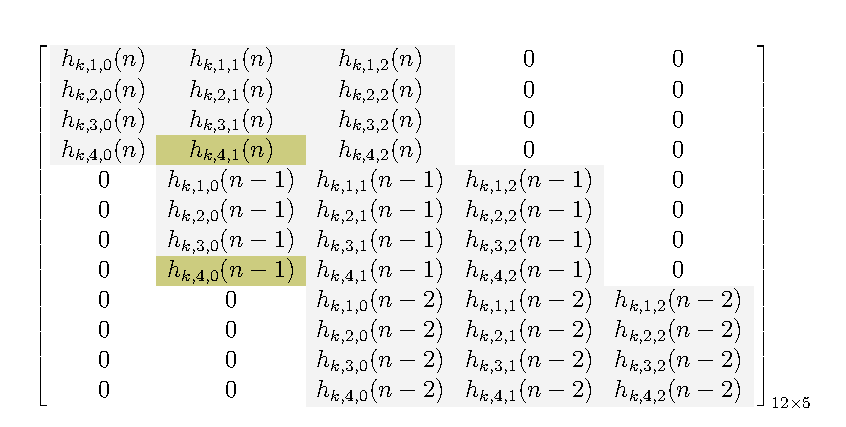
\includegraphics[width=\columnwidth]{colArray}

%\[
%\left[\,
%\begin{array}{*{5}{>{\columncolor[gray]{0.95}}c}}
%  {h_{k,1,0}(n)} & {h_{k,1,1}(n)} & {h_{k,1,2}(n)} & \zero & \zero \\
%  {h_{k,2,0}(n)} & {h_{k,2,1}(n)} & {h_{k,2,2}(n)} & \zero & \zero \\
%  {h_{k,3,0}(n)} & {h_{k,3,1}(n)} & {h_{k,3,2}(n)} & \zero & \zero \\
%  {h_{k,4,0}(n)} & \colCell{umbra}{h_{k,4,1}(n)} & {h_{k,4,2}(n)} & \zero & \zero \\
%  \zero & {h_{k,1,0}(n-1)} & {h_{k,1,1}(n-1)} & {h_{k,1,2}(n-1)} & \zero \\
%  \zero & {h_{k,2,0}(n-1)} & {h_{k,2,1}(n-1)} & {h_{k,2,2}(n-1)} & \zero \\
%  \zero & {h_{k,3,0}(n-1)} & {h_{k,3,1}(n-1)} & {h_{k,3,2}(n-1)} & \zero \\
%  \zero & \colCell{umbra}{h_{k,4,0}(n-1)} & {h_{k,4,1}(n-1)} & {h_{k,4,2}(n-1)} & \zero \\
%  \zero & \zero & {h_{k,1,0}(n-2)} & {h_{k,1,1}(n-2)} & {h_{k,1,2}(n-2)}\\
%  \rowcolor[gray]{0.75}%
%  \zero & \zero & {h_{k,2,0}(n-2)} & {h_{k,2,1}(n-2)} & {h_{k,2,2}(n-2)}\\
%  \zero & \zero & {h_{k,3,0}(n-2)} & {h_{k,3,1}(n-2)} & {h_{k,3,2}(n-2)}\\
%  \zero & \zero & {h_{k,4,0}(n-2)} & {h_{k,4,1}(n-2)} & {h_{k,4,2}(n-2)}
%\end{array} \,\right]
%\end]


\medskip
\begin{lstlisting}[xrightmargin=-\marginparwidth]
...
\usepackage{array}
\usepackage{colortbl}
\definecolor{umbra}{rgb}{0.8,0.8,0.5}
\def\zero{\multicolumn{1}{>{\columncolor{white}}c}{0}}
\def\colCell#1#2{\multicolumn{1}{>{\columncolor{#1}}c}{#2}}
\begin{document}
\[\left[\,
\begin{array}{*{5}{>{\columncolor[gray]{0.95}}c}}
  h_{k,1,0}(n) & h_{k,1,1}(n) & h_{k,1,2}(n) & \zero & \zero\\
  h_{k,2,0}(n) & h_{k,2,1}(n) & h_{k,2,2}(n) & \zero & \zero\\
  h_{k,3,0}(n) & h_{k,3,1}(n) & h_{k,3,2}(n) & \zero & \zero\\
  h_{k,4,0}(n)} & \colCell{umbra}{h_{k,4,1}(n)} & h_{k,4,2}(n) & \zero & \zero\\
  \zero & h_{k,1,0}(n-1) & h_{k,1,1}(n-1) & h_{k,1,2}(n-1) & \zero\\
  \zero & h_{k,2,0}(n-1) & h_{k,2,1}(n-1) & h_{k,2,2}(n-1) & \zero\\
  \zero & h_{k,3,0}(n-1) & h_{k,3,1}(n-1) & h_{k,3,2}(n-1) & \zero\\
  \zero & \colCell{umbra}{h_{k,4,0}(n-1)} & h_{k,4,1}(n-1) & h_{k,4,2}(n-1) & \zero\\
  \zero & \zero & h_{k,1,0}(n-2) & h_{k,1,1}(n-2) & h_{k,1,2}(n-2)\\
  \zero & \zero & h_{k,2,0}(n-2) & h_{k,2,1}(n-2) & h_{k,2,2}(n-2)\\
  \zero & \zero & h_{k,3,0}(n-2) & h_{k,3,1}(n-2) & h_{k,3,2}(n-2)\\
  \zero & \zero & h_{k,4,0}(n-2) & h_{k,4,1}(n-2) & h_{k,4,2}(n-2)
\end{array} \,\right]_{12\times 5}\]
...
\end{lstlisting}


\subsection{Boxed rows and columns}

\begin{LTXexample}[width=0.35\linewidth]
\[
\overrightarrow{A}=\left[
    \begin{array}{cccc}
	1 & 2 & 3 & 4\\
	1 & 2 & 3 & 4\\\hline
	\multicolumn{1}{|c}{1} & 2 & 3 & 
	\multicolumn{1}{c|}{4}\\\hline
	1 & 2 & 3 & 4
    \end{array}\right]
\]
\end{LTXexample}


\begin{LTXexample}[width=0.35\linewidth]
\[
\overrightarrow{A}=\left[
    \begin{array}{cc|c|c}\cline{3-3}
	1 & 2 & 3 & 4\\
	1 & 2 & 3 & 4\\
	1 & 2 & 3 & 4\\
	1 & 2 & 3 & 4\\\cline{3-3}
    \end{array}\right]
\]
\end{LTXexample}

\begin{LTXexample}[width=0.35\linewidth]
\[
\overrightarrow{A}=\left[
    \begin{array}{cc|c|c}\cline{3-3}
	1 & 2 & 3 & 4\\
	1 & 2 & 3 & 4\\\hline
	\multicolumn{1}{|c}{1} & 2 & 3 & 
	\multicolumn{1}{c|}{4}\\\hline
	1 & 2 & 3 & 4\\\cline{3-3}
    \end{array}\right]
\]
\end{LTXexample}



\section{Over- and underbraces}
\subsection{Braces and roots}
To put an underbrace in a root without enlarging the root symbol is possible with
the \verb+\makebox+ macro:

\[ z =\;\;\underbrace{\makebox[\widthof{~$x^2+y^2$}][r]{$\sqrt{x^2+y^2}$}}_{=z^2} \]

\begin{lstlisting}
\[
z =\;\;\underbrace{%
  \makebox[\widthof{~$x^2+y^2$}][r]{%
     $\sqrt{x^2+y^2}$}}_{=z^2}
\]
\end{lstlisting}



\subsection{Overlapping braces}
Overlapping under- and overbraces like%
\parbox{10em}{\begin{align*}
\qquad\overbrace{\qquad\qquad}^o\qquad\\[-16pt]
\underbrace{\qquad\qquad}_{u1}\underbrace{\qquad\qquad}_{u2}
\end{align*}} needs some tricky code, because we cannot have parts of the argument inside
\verb+overbrace+\index{overbrace@\textbackslash overbrace} and also \verb+underbrace+.
\index{underbrace@\textbackslash underbrace} The following equation~\vref{eq:pqFormel}
is an example for such a construction:

\begin{align}\label{eq:pqFormel}
y &= 2x^2 -3x +5\nonumber\\
  & \hphantom{= \ 2\left(x^2-\frac{3}{2}\,x\right. }%
         \textcolor{blue}{%
              \overbrace{\hphantom{+\left(\frac{3}{4}\right)^2- %
                  \left(\frac{3}{4}\right)^2}}^{=0}}\nonumber\\[-11pt]
  &= 2\left(\textcolor{red}{%
     \underbrace{%
         x^2-\frac{3}{2}\,x + \left(\frac{3}{4}\right)^2}%
     }%
     \underbrace{%
        - \left(\frac{3}{4}\right)^2 + \frac{5}{2}}%
     \right)\\
  &= 2\left(\qquad\textcolor{red}{\left(x-\frac{3}{4}\right)^2}
     \qquad + \ \frac{31}{16}\qquad\right)\nonumber\\
y\textcolor{blue}{-\frac{31}{8}}
  &= 2\left(x\textcolor{cyan}{-\frac{3}{4}}\right)^2\nonumber
\end{align}

\medskip%[xrightmargin=-\marginparwidth]
\begin{lstlisting}
\begin{align}\label{eq:pqFormel}
y &= 2x^2 -3x +5\nonumber\\
  & \hphantom{= \ 2\left(x^2-\frac{3}{2}\,x\right. }%
         \textcolor{blue}{%
              \overbrace{\hphantom{+\left(\frac{3}{4}\right)^2- %
                  \left(\frac{3}{4}\right)^2}}^{=0}}\nonumber\\[-11pt]
  &= 2\left(\textcolor{red}{%
     \underbrace{%
         x^2-\frac{3}{2}\,x + \left(\frac{3}{4}\right)^2}%
     }%
     \underbrace{%
        - \left(\frac{3}{4}\right)^2 + \frac{5}{2}}%
     \right)\\
  &= 2\left(\qquad\textcolor{red}{\left(x-\frac{3}{4}\right)^2}
     \qquad + \ \frac{31}{16}\qquad\right)\nonumber\\
y\textcolor{blue}{-\frac{31}{8}}
  &= 2\left(x\textcolor{cyan}{-\frac{3}{4}}\right)^2\nonumber
\end{align}
\end{lstlisting}

\subsection[Vertical alignment]{Vertical alignment of different braces}
When having several braces in one formula line, then it looks better when all
braces are also on the same line, \eg

\begin{equation}
	\binom{x_R}{y_R} = \underbrace{r\vphantom{\binom{A}{B}}}_{\text{Scaling}}\cdot%
    \underbrace{%
		\begin{pmatrix}
    		\sin \gamma & -\cos \gamma \\
    		\cos \gamma & \sin \gamma \\
		\end{pmatrix}%
    }_{\text{Rotation}}
	\binom{x_K}{y_K} +
    \underbrace{\binom{t_x}{t_y}}_{\text{Translation}}
\end{equation}
%[xrightmargin=-\marginparwidth]
\begin{lstlisting}
\begin{equation}
\binom{x_R}{y_R} = \underbrace{r\vphantom{\binom{A}{B}}}_{\text{Skaling}}\cdot%
    \underbrace{%
	\begin{pmatrix}
    		\sin \gamma & -\cos \gamma \\
    		\cos \gamma & \sin \gamma \\
	\end{pmatrix}%
    }_{\text{Rotation}}
\binom{x_K}{y_K} + \underbrace{\binom{t_x}{t_y}}_{\text{Translation}}
\end{equation}
\end{lstlisting}

It is again the \verb+\vphantom+ macro which reserves the needed vertical space.
Nevertheless the horizontal space around the \verb+r+ of the first underbrace and the last \verb|+| should
be decreased to get a better typesetting. This is possible with \verb+\hspace+ or
simply \verb+\kern+:

\[ \binom{x_R}{y_R} = %
    \kern-10pt\underbrace{r\vphantom{\binom{A}{B}}}_{\text{Skaling}}\kern-10pt%
    \cdot\underbrace{%
      \begin{pmatrix}
        \sin \gamma & -\cos \gamma \\
        \cos \gamma & \sin \gamma \\
      \end{pmatrix}%
    }_{\text{Rotation}}
  \binom{x_K}{y_K} +\kern-5pt%
  \underbrace{\binom{t_x}{t_y}}_{\text{Translation}} \]
%[xrightmargin=-\marginparwidth]
\begin{lstlisting}
\[ \binom{x_R}{y_R} = %
    \kern-10pt\underbrace{r\vphantom{\binom{A}{B}}}_{\text{Skaling}}\kern-10pt%
    \cdot\underbrace{%
      \begin{pmatrix}
        \sin \gamma & -\cos \gamma \\
        \cos \gamma & \sin \gamma \\
      \end{pmatrix}%
    }_{\text{Rotation}}
  \binom{x_K}{y_K} +\kern-5pt%
  \underbrace{\binom{t_x}{t_y}}_{\text{Translation}} \]
\end{lstlisting}


\subsection[Alignment]{Vertical and horizontal alignment}
The forgoing example simply uses \verb+\hspace+ to decrease the horizontal width between two
\index{underbrace@\textbackslash underbrace} underbraces. This may be okay for a single solution, but in general it is better to have some    %%% ----- Martin -----
code which works in any case.

The following example looks simple but it needs some tricky code to get vertical and horizontal
alignment.\index{substack@\textbackslash substack}

\def\num#1{\hphantom{#1}}
\def\vsp{\vphantom{\rangle_1}}

\begin{equation*}
    \frac{300}{5069}%
    \underbrace{\longmapsto\vphantom{\frac{1}{1}}}_{%
	   \mathclap{\substack{%
	     \Delta a=271\num9\vsp \\[2pt]
	     \Delta b=4579\vsp\\[2pt]
	     \text{$1$ iteration}%
	   }}} \frac{29}{490}%
	\underbrace{\longmapsto \frac{19}{321}\longmapsto}_{%
      \mathclap{\substack{%
	     \Delta a=10\num{9}=\langle271\rangle_{29}\num{20}\\[2pt]
         \Delta b=169=\langle4579\rangle_{490}\\[2pt]
         \text{$2$ iterations}
      }}} \frac{9}{152}
    \underbrace{\longmapsto \frac{8}{135}\longmapsto\dots\longmapsto}_{%
      \substack{%
	    \Delta a=1\num{7}=\langle10\rangle_{9}\num{119}\\[2pt]
	    \Delta b=17=\langle169\rangle_{152}\\[2pt]
	    \text{$8$ iterations}
      }} \frac{1}{16}
    \underbrace{\longmapsto\dots\longmapsto\vphantom{\frac{8}{135}}}_{%
      \substack{%
	     \Delta a=0=\langle1\rangle_{1}\num{76} \\[2pt]
	     \Delta b=1=\langle17\rangle_{16} \\[2pt]
         \text{$8$ iterations}
      }} \frac{1}{1}
\end{equation*}

It uses the macro \verb+\mathclap+ defined in section\vref{subsec:ams-limits}
\index{mathclap@\textbackslash mathclap}\index{vphantom@\textbackslash vphantom}\index{hphantom@\textbackslash hphantom}
, which gives a better result.    %%% ----- Martin -----
It is also possible to use \verb+\makebox[0pt]{...}+ but it works only in text mode
and this needs some more \verb+$...$+.\index{substack@\textbackslash substack}

%[xrightmargin=-\marginparwidth]
\begin{lstlisting}
\def\num#1{\hphantom{#1}}
\def\vsp{\vphantom{\rangle_1}}

\begin{equation*}
    \frac{300}{5069}%
    \underbrace{\longmapsto\vphantom{\frac{1}{1}}}_{%
	   \mathclap{\substack{%
	     \Delta a=271\num9\vsp \\[2pt]
	     \Delta b=4579\vsp\\[2pt]
	     \text{$1$ iteration}%
	   }}} \frac{29}{490}%
	\underbrace{\longmapsto \frac{19}{321}\longmapsto}_{%
      \mathclap{\substack{%
	     \Delta a=10\num{9}=\langle271\rangle_{29}\num{20}\\[2pt]
         \Delta b=169=\langle4579\rangle_{490}\\[2pt]
         \text{$2$ iterations}
      }}} \frac{9}{152}
    \underbrace{\longmapsto \frac{8}{135}\longmapsto\dots\longmapsto}_{%
      \substack{%
	    \Delta a=1\num{7}=\langle10\rangle_{9}\num{119}\\[2pt]
	    \Delta b=17=\langle169\rangle_{152}\\[2pt]
	    \text{$8$ iterations}
      }} \frac{1}{16}
    \underbrace{\longmapsto\dots\longmapsto\vphantom{\frac{8}{135}}}_{%
      \substack{%
	     \Delta a=0=\langle1\rangle_{1}\num{76} \\[2pt]
	     \Delta b=1=\langle17\rangle_{16} \\[2pt]
         \text{$8$ iterations}
      }} \frac{1}{1}
\end{equation*}
\end{lstlisting}


\section{Integrals}\label{sec:Integrals}
\index{underset@\textbackslash underset}
\def\Q#1#2{\frac{\partial #1}{\partial #2}}
%
The \emph{first theorem of Green} is:
\[
\underset{\mathcal{G}\quad}\iiint\!%
	\left[u\nabla^{2}v+\left(\nabla u,\nabla v\right)\right]\mathrm{d}^{3}V%
	=\underset{\mathcal{S}\quad}\oiint u\,\Q{v}{n}\,\,\mathrm{d}^{2}A
\]

The \emph{second theorem of Green} is:

\[
\underset{{\mathcal{G}\quad}}\iiint\!%
	\left[u\nabla^{2}v-v\nabla^{2}u\right]\mathrm{d}^{3}V%
	=\underset{\mathcal{S}\quad}\oiint%
	\left(u\,\Q{v}{n}-v\,\Q{u}{n}\right)\mathrm{d}^{2}A
\]


They are both written with the \PIndex{esint} package%
\footnote{See section~\vref{sec:Integrals}.}, which gives nice integral symbols.  
The \LaTeX{} code for the first equation is:

%[xrightmargin=-\marginparwidth]
\begin{lstlisting}
\[
\underset{\mathcal{G}\quad}\iiint\!%
  \left[u\nabla^{2}v+\left(\nabla u,\nabla v\right)\right]\mathrm{d}^{3}V%
  =\underset{\mathcal{S}\quad}\oiint u\,\Q{v}{n}\,\,\mathrm{d}^{2}A
\]
\end{lstlisting}

\noindent with the following definition in the preamble for the partial derivation:

\begin{lstlisting}
\def\Q#1#2{\frac{\partial#1}{\partial #2}}
\end{lstlisting}

\noindent which makes things easier to write.

%--------------------------------------------------------------------------
\section{Horizontal alignment}\label{sec:verticalAlignment}
%--------------------------------------------------------------------------
\subsection{Over more than one page}
%--------------------------------------------------------------------------
Sometimes it may be useful to have a vertical alignment over the whole page with a mix of    %%% ----- Martin -----
formulas and text. Section \ref{sec:Text-in-math mode} shows the use of \CMD{intertext}.
There is another trick to get all formulas vertical aligned.  Let's have the following
formulas distributed over the whole page:
%
\begin{align*}
     f(x) &= a\\
     g(x) &= x^2-4x\\
f(x)-g(x) &= x^2+x^3+x\\
     g(x) &= x^2+x^3+x^4+x^5+b
\end{align*}
%
They all have a different length of the left and right side. Now we want to write some
text and other objects between them, but let the alignment untouched. We choose the
longest left and the longest right side and take them for scaling with the \CMD{hphantom}
command:

\begin{verbatim}
\hphantom{\mbox{$f(x)-g(x)$}} & \hphantom{\mbox{$= x^2+x^3+x^4+x^5+b$}}
\end{verbatim}

This is the first (empty) line in every equation where now all other lines are aligned to
this one. For example:

\bgroup
\medskip\noindent
\rule{\columnwidth}{1pt}
\newcommand\x{blah blah blah blah blah blah blah blah }
\addtolength\abovedisplayshortskip{-.5cm}% decrease the skip
\addtolength\abovedisplayskip{-.5cm}
\x\x\x
\begin{align}
\hphantom{\mbox{$f(x)-g(x)$}} & \hphantom{\mbox{$= x^2+x^3+x^4+x^5+b$}}\nonumber\\
f(x) &= a\\
g(x) &= x^2-4x
\end{align}
%
\x\x\x
\begin{align}
\hphantom{\mbox{$f(x)-g(x)$}} & \hphantom{\mbox{$= x^2+x^3+x^4+x^5+b$}}\nonumber\\
f(x)-g(x) &= x^2+x^3+x
\end{align}
\x\x\x
%
\begin{align}
\hphantom{\mbox{$f(x)-g(x)$}} & \hphantom{\mbox{$= x^2+x^3+x^4+x^5+b$}}\nonumber\\
g(x) &= x^2+x^3+x^4+x^5+b
\end{align}
\x\x\x

\noindent
\rule{\columnwidth}{1pt}
\egroup
\medskip

The phantom line is empty but leaves the vertical space for a line. This could be
corrected with decreasing the \CMD{abovedisplayshortskip} length and done all
inside a group.

%[xrightmargin=-\marginparwidth]
\begin{lstlisting}
\newcommand\x{blah blah blah blah blah blah blah blah }
\bgroup
\addtolength\abovedisplayshortskip{-0.5cm}% decrease the skip
\addtolength\abovedisplayskip{-0.5cm}
\x\x\x
\begin{align}
\hphantom{\mbox{$f(x)-g(x)$}} & \hphantom{\mbox{$= x^2+x^3+x^4+x^5+b$}}\nonumber\\
f(x) &= a\\
g(x) &= x^2-4x
\end{align}
%
\x\x\x
\begin{align}
\hphantom{\mbox{$f(x)-g(x)$}} & \hphantom{\mbox{$= x^2+x^3+x^4+x^5+b$}}\nonumber\\
f(x)-g(x) &= x^2+x^3+x
\end{align}
\x\x\x
%
\begin{align}
\hphantom{\mbox{$f(x)-g(x)$}} & \hphantom{\mbox{$= x^2+x^3+x^4+x^5+b$}}\nonumber\\
g(x) &= x^2+x^3+x^4+x^5+b
\end{align}
\x\x\x
\egroup
\end{lstlisting}




Another case of aligning equations inside an itemize environment is the following one.
With the \CIndex{makebox} macro one can have the same size on the left side of the
equal sign to get a vertical alignment.

\newsavebox\lW
\sbox\lW{$P_{3}+P_{2}-P_{1}$}%  $

\begin{itemize}
\item first function \\
  $\displaystyle\makebox[\wd\lW][r]{$P_1$}=\sum_a \in A$
\item but another one \\
  $\makebox[\wd\lW][r]{$\sin\left(P_1\right)$}=blabla$
\item or perhaps \\
  $P_{3}+P_{2}-P_{1}=blablub$
\end{itemize}

%[xrightmargin=-\marginparwidth]
\begin{lstlisting}
\newsavebox\lW
\sbox\lW{$P_{3}+P_{2}-P_{1}$}

\begin{itemize}
\item first function \\
  $\displaystyle\makebox[\wd\lW][r]{$P_1$}=\sum_a \in A$
\item but another one \\
  $\makebox[\wd\lW][r]{$\sin\left(P_1\right)$}=blabla$
\item or perhaps \\
  $P_{3}+P_{2}-P_{1}=blablub$
\end{itemize}
\end{lstlisting}
%$

%--------------------------------------------------------------------------
\subsection{Special text columns}
%--------------------------------------------------------------------------
This one comes from Hartmut Henkel and offers a special form of placing
additional text between the equation and the \Index{equation number}. This makes only
sense when you load the documentclass with the option \verb+fleqn+. The example
places the additional text at \verb+0.5\textwidth+, changing this value is no
problem.

\clearpage
\medskip
\noindent\rule{\linewidth}{1pt}
\begingroup
\small
text text text text text text text text text text text text text text
text text text text text text text text text text text text text text
text text text text text text text text text text text text text text
text text text text text text text text text text text text text text

\makeatletter
\@fleqntrue
\let\old@mathmargin=\@mathmargin
\@mathmargin=-1sp
\let\oldmathindent=\mathindent
\let\mathindent=\@mathmargin
\newsavebox{\myendhook} % for the tabulars
\def\tagform@#1{{(\maketag@@@{\ignorespaces#1\unskip\@@italiccorr)}
  \makebox[0pt][r]{% after the equation number
    \makebox[0.5\textwidth][l]{\usebox{\myendhook}}}%
  \global\sbox{\myendhook}{}% empty box
}}
\makeatother
\sbox{\myendhook}{%
\begin{footnotesize}%
\begin{tabular}{@{}ll}
$a_0$ & Bohrscher Radius ($\mathrm{= 0{,}53\,\mbox{\AA}}$)\\
$e$ & Elementarladung\\
$N_{si}$ & Anzahl der Siliziumatome\\
& pro Einheitsvolumen\\
$m$ & Atomgewicht\\
$Z$ & Kernladungszahl
\end{tabular}
\end{footnotesize}}
%
\begin{equation}
\varepsilon = \frac{E \cdot 4 \cdot \pi \cdot \varepsilon_{0}
\cdot a_0 \cdot \left( Z_i^{\frac{2}{3}} + Z_{Si}^{\frac{2}{3}}
\right)^{-\frac{1}{2}}} {Z_i \cdot Z_{Si} \cdot e2 \cdot \left( 1
+ \frac{m_i}{m_{Si}} \right)}\,;
\end{equation}

\sbox{\myendhook}{abc}

\begin{equation}
a2+b2=c2
\end{equation}

\begin{equation}
z = 9
\end{equation}
text text text text text text text text text text text text text text
text text text text text text text text text text text text text text
text text text text text text text text text text text text text text
text text text text text text text text text text text text text text

\endgroup
\noindent\rule{\linewidth}{1pt}

\medskip
This solution works only with \AmSmath{}, without you have to redefine the
\LaTeX{} macro, which creates the equation number.

%[xrightmargin=-\marginparwidth]
\begin{lstlisting}
\newsavebox{\myendhook} % for the tabulars
\def\tagform@#1{{(\maketag@@@{\ignorespaces#1\unskip\@@italiccorr)}
  \makebox[0pt][r]{% after the equation number
    \makebox[0.4\textwidth][l]{\usebox{\myendhook}}%
  }%
  \global\sbox{\myendhook}{}% clear box content
}}
[ ... ]
\sbox{\myendhook}{%
\begin{footnotesize}%
\begin{tabular}{@{}ll}
$a_0$ & Bohrscher Radius ($\mathrm{= 0{,}53\,\mbox{\AA}}$)\\
$e$ & Elementarladung\\
$N_{si}$ & Anzahl der Siliziumatome\\
& pro Einheitsvolumen\\
$m$ & Atomgewicht\\
$Z$ & Kernladungszahl
\end{tabular}
\end{footnotesize}}
%
\begin{equation}
\varepsilon = \frac{E \cdot 4 \cdot \pi \cdot \varepsilon_{0}
\cdot a_0 \cdot \left( Z_i^{\frac{2}{3}} + Z_{Si}^{\frac{2}{3}}
\right)^{-\frac{1}{2}}} {Z_i \cdot Z_{Si} \cdot e2 \cdot \left( 1
+ \frac{m_i}{m_{Si}} \right)}\,;
\end{equation}
%
\sbox{\myendhook}{abc}
%
\begin{equation} a2+b2=c2  \end{equation}
%
\begin{equation} z = 9 \end{equation}
\end{lstlisting}


%--------------------------------------------------------------------------
\subsection{Centered vertical dots}
%--------------------------------------------------------------------------

By default the vertical dots of \CMD{vdots} are aligned to the left of 
the $=$ symbol and not centered.\index{vdots@\textbackslash vdots}
%
\bgroup
\newsavebox{\eqbox}% Heiko Bauke
\sbox{\eqbox}{$\null=\null$}
\newcommand\Vdots{\makebox[\wd\eqbox]{\vdots}}
%
\begin{align}
  a_1 & = b_1    & c_1 & = d_1 \\
  a_2 & = b_2    & c_2 & = d_2 \\
  a   & \Vdots b &     & \Vdots \nonumber \\
  a_n & = b_n    & c_n & = d_n 
\end{align}
\egroup
%
\begin{lstlisting}
\usepackage{amsmath}
...

\newsavebox{\eqbox}
\sbox{\eqbox}{$\null=\null$}
\newcommand\Vdots{\makebox[\wd\eqbox]{\vdots}}

\begin{align}
  a_1 & = b_1    & c_1 & = d_1 \\
  a_2 & = b_2    & c_2 & = d_2 \\
  a   & \Vdots b &     & \Vdots \nonumber \\
  a_n & = b_n    & c_n & = d_n 
\end{align}
\end{lstlisting}


%------------------------------------------------------------------------------
\section{Node connections}
%------------------------------------------------------------------------------
This is a typical application for PSTricks and it needs the package \verb+pst-node+
and doesn't work with \verb+pdflatex+. Use \verb+vlatex+, \verb+ps4pdf+ or \verb+ps2pdf+.

\medskip
\noindent\fbox{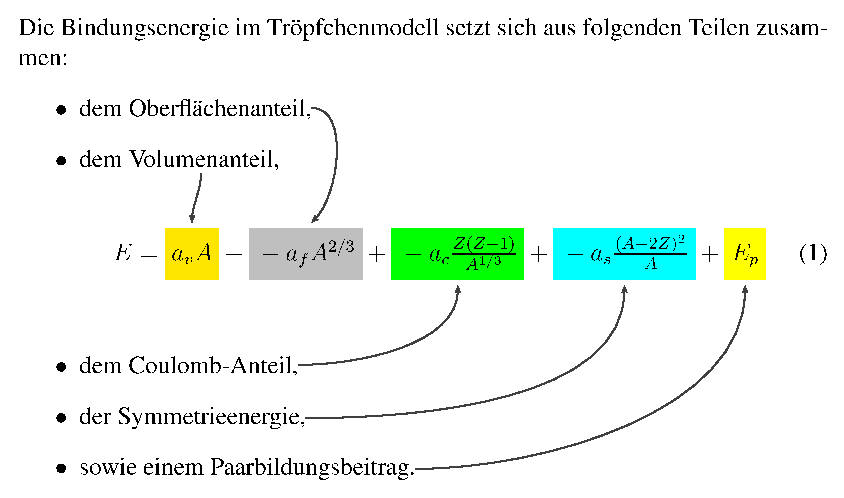
\includegraphics[width=\linewidth]{node}}

\iffalse
\noindent\fbox{\parbox{\linewidth-2\fboxsep-2\fboxrule}{%
\psset{nodesep=3pt}
\definecolor{lila}{rgb}{0.6,0.2,0.5}
\definecolor{darkyellow}{rgb}{1,0.9,0}
Die Bindungsenergie im Tr\"opfchenmodell setzt sich aus
folgenden Teilen zusammen:
\begin{itemize}
\item dem \rnode{b}{Oberfl\"achenanteil}
\item dem \rnode{a}{Volumenanteil},\\[0.75cm]
\def\xstrut{\vphantom{\frac{(A)^1}{(B)^1}}}
\begin{equation}
E =
\rnode[t]{ae}{\psframebox*[fillcolor=darkyellow,
  linestyle=none]{\xstrut a_vA}} +
\rnode[t]{be}{\psframebox*[fillcolor=lightgray,
  linestyle=none]{\xstrut -a_fA^{2/3}}} +
\rnode[t]{ce}{\psframebox*[fillcolor=green,
  linestyle=none]{\xstrut -a_c\dfrac{Z(Z-1)}{A^{1/3}}}} +
\rnode[t]{de}{\psframebox*[fillcolor=cyan,
  linestyle=none]{\xstrut -a_s\frac{(A-2Z)^2}{A}}} +
\rnode[t]{ee}{\psframebox*[fillcolor=yellow,
  linestyle=none]{\xstrut E_p}}
\end{equation}\\
\item dem \rnode{c}{Coulomb-Anteil}
\item der \rnode{d}{Symmetrieenergie}
\item sowie einem \rnode{e}{Paarbildungsbeitrag}.
\end{itemize}
\nccurve[angleA=-90,angleB=90]{->}{a}{ae}
\nccurve[angleB=45]{->}{b}{be}
\nccurve[angleB=-90]{->}{c}{ce}
\nccurve[angleB=-90]{->}{d}{de}
\nccurve[angleB=-90]{->}{e}{ee}
}}
\fi

\medskip
%,xrightmargin=-\marginparwidth
\begin{lstlisting}[tabsize=4]
\psset{nodesep=3pt}
\definecolor{lila}{rgb}{0.6,0.2,0.5}
\definecolor{darkyellow}{rgb}{1,0.9,0}
Die Bindungsenergie im Tr\"opfchenmodell setzt sich aus
folgenden Teilen zusammen:
\begin{itemize}
\item dem \rnode{b}{Oberfl\"achenanteil}
\item dem \rnode{a}{Volumenanteil},\\[1cm]
\def\xstrut{\vphantom{\frac{(A)^1}{(B)^1}}}
\begin{equation}
E =
\rnode[t]{ae}{\psframebox*[fillcolor=darkyellow,
  linestyle=none]{\xstrut a_vA}} +
\rnode[t]{be}{\psframebox*[fillcolor=lightgray,
  linestyle=none]{\xstrut -a_fA^{2/3}}} +
\rnode[t]{ce}{\psframebox*[fillcolor=green,
  linestyle=none]{\xstrut -a_c\frac{Z(Z-1)}{A^{1/3}}}} +
\rnode[t]{de}{\psframebox*[fillcolor=cyan,
  linestyle=none]{\xstrut -a_s\frac{(A-2Z)^2}{A}}} +
\rnode[t]{ee}{\psframebox*[fillcolor=yellow,
  linestyle=none]{\xstrut E_p}}
\end{equation}\\[0.25cm]
\item dem \rnode{c}{Coulomb-Anteil}
\item der \rnode{d}{Symmetrieenergie}
\item sowie einem \rnode{e}{Paarbildungsbeitrag}.
\end{itemize}
\nccurve[angleA=-90,angleB=90]{->}{a}{ae}
\nccurve[angleB=45]{->}{b}{be}  \nccurve[angleB=-90]{->}{c}{ce}
\nccurve[angleB=-90]{->}{d}{de} \nccurve[angleB=-90]{->}{e}{ee}
\end{lstlisting}




%-----------------------------------------------------------------------------
\section[Special Placement]{Special placement of displayed equations}
%-----------------------------------------------------------------------------

%-----------------------------------------------------------------------------
\subsection{Formulas side by side}\label{sec:sidebyside}
%-----------------------------------------------------------------------------

Sometimes it may be useful to have numbered formulas side by side like the following ones:

%\begin{framed}
\begin{mtabular}{*{2}{m{0.35\linewidth}m{0.15\linewidth}}}
\begin{align*} \oint E ds=0 \end{align*} & \eqnCnt %
	& \begin{align*} \nabla\cdot B=0 \end{align*} & \eqnCnt[\label{blah}]\\
\begin{align*} a =\frac{c}{d} \end{align*} & \eqnCnt %
	& \begin{align*} b = 1 \end{align*} & \eqnCnt\\
\begin{align*} c =1 \end{align*} & \eqnCnt[\label{blub}]
	& \begin{align*} \int 2x \,\mathrm{d}x = x^2+C \end{align*} & \eqnCnt
\end{mtabular}
%\end{framed}


And again a default display equation:
\begin{align}
F(x) &= \int_0^\infty\dfrac{1}{x}\,\mathrm{d}x
\end{align}

%,xrightmargin=-\marginparwidth
\begin{lstlisting}[tabsize=4]
\begin{mtabular}{*{2}{m{0.35\linewidth}m{0.15\linewidth}}}
\begin{align*} \oint E ds=0 \end{align*} & \eqnCnt %
	& \begin{align*} \nabla\cdot B=0 \end{align*} & \eqnCnt[\label{blah}]\\
\begin{align*} a =\frac{c}{d} \end{align*} & \eqnCnt %
	& \begin{align*} b = 1 \end{align*} & \eqnCnt\\
\begin{align*} c =1 \end{align*} & \eqnCnt[\label{blub}]
	& \begin{align*} \int 2x \,\mathrm{d}x = x^2+C \end{align*} & \eqnCnt
\end{mtabular}
\end{lstlisting}

The new environment \verb|mtabular| has two arguments, one optional and one which is the same
as the one from the \verb|tabular| environment. With the option \verb|long| it is possible to have    %%% ----- Martin -----
all the formulas in a \verb|longtable| environment, which allows a pagebreak. The new macro
\verb|\eqnCnt| controls the counting of these equations as subequations for one tabular
line. This macro can have an optional argument for a label. At least it counts 
the equations. If the
equation number is not centered to the foregoing equation, then it needs some more horizontal
space in the tabular column.

\begin{verbatim}
\eqnCnt[<optional label>]
\end{verbatim}

The vertical space is controlled by the length \verb|\mtabskip|, which 
is by default \verb|-1.25cm| and can be modified in the usual way.
To define all these macros write into the preamble:

%,xrightmargin=-\marginparwidth
\begin{lstlisting}[tabsize=4]
\usepackage{amsmath}
\newcounter{subequation}
\newlength\mtabskip\mtabskip=-1.25cm
\newcommand\eqnCnt[1][]{%
	\refstepcounter{subequation}%
	\begin{align}#1\end{align}%
	\addtocounter{equation}{-1}}
\def\mtabLong{long}
\makeatletter
\newenvironment{mtabular}[2][\empty]{%
	\def\@xarraycr{%
		\stepcounter{equation}%
		\setcounter{subequation}{0}%
		\@ifnextchar[\@argarraycr{\@argarraycr[\mtabskip]}}
	\let\theoldequation\theequation%
	\renewcommand\theequation{\theoldequation.\alph{subequation}}
	\edef\mtabOption{#1}
	\setcounter{subequation}{0}%
	\tabcolsep=0pt
	\ifx\mtabOption\mtabLong\longtable{#2}\else\tabular{#2}\fi%
}{%
	\ifx\mtabOption\mtabLong\endlongtable\else\endtabular\fi%
	\let\theequation\theoldequation%
	\stepcounter{equation}}
\makeatother
\end{lstlisting}


As seen in equation~\ref{blub} and equation~\ref{blah}, everything of the table contents is 
nonsense~\ldots And the following tabular is defined as a \Index{longtable} to enable pagebreaks.
%which is the reason for the following big skip, to show that it works.


%\vspace*{3cm}
%\begin{framed}
\begin{mtabular}[long]{*{2}{m{0.35\linewidth}m{0.15\linewidth}}}
\begin{align*} \oint E ds=0 \end{align*} & \eqnCnt %
	& \begin{align*} \nabla\cdot B=0 \end{align*} & \eqnCnt\\
\begin{align*} a =\frac{c}{d} \end{align*} & \eqnCnt %
	& \begin{align*} b = 1 \end{align*} & \eqnCnt\\
\begin{align*} c =1 \end{align*} & \eqnCnt
	& \begin{align*} \int 2x \,\mathrm{d}x = x^2+C \end{align*} & \eqnCnt\\
\begin{align*} \oint E ds=0 \end{align*} & \eqnCnt %
	& \begin{align*} \nabla\cdot B=0 \end{align*} & \eqnCnt\\
\begin{align*} a =\frac{c}{d} \end{align*} & \eqnCnt %
	& \begin{align*} b = 1 \end{align*} & \eqnCnt\\
\begin{align*} c =1 \end{align*} & \eqnCnt
	& \begin{align*} \int 2x \,\mathrm{d}x = x^2+C \end{align*} & \eqnCnt\\
\begin{align*} \oint E ds=0 \end{align*} & \eqnCnt %
	& \begin{align*} \nabla\cdot B=0 \end{align*} & \eqnCnt[\label{blah2}]\\
\begin{align*} a =\frac{c}{d} \end{align*} & \eqnCnt %
	& \begin{align*} b = 1 \end{align*} & \eqnCnt\\
\begin{align*} c =1 \end{align*} & \eqnCnt[\label{blub2}]
	& \begin{align*} \int 2x \,\mathrm{d}x = x^2+C \end{align*} & \eqnCnt\\
\begin{align*} \oint E ds=0 \end{align*} & \eqnCnt %
	& \begin{align*} \nabla\cdot B=0 \end{align*} & \eqnCnt\\
\begin{align*} a =\frac{c}{d} \end{align*} & \eqnCnt %
	& \begin{align*} b = 1 \end{align*} & \eqnCnt\\
\begin{align*} c =1 \end{align*} & \eqnCnt
	& \begin{align*} \int 2x \,\mathrm{d}x = x^2+C \end{align*} & \eqnCnt
\end{mtabular}
%\end{framed}

As seen in equation~\ref{blub2} and equation~\ref{blah2}, everything is nonsense ...


And again a default display equation:
\begin{align}
F(x) &= \int_0^\infty\dfrac{1}{x}\,\mathrm{d}x
\end{align}

\begin{lstlisting}[tabsize=4]
\begin{mtabular}[long]{*{2}{m{0.375\linewidth}m{0.125\linewidth}}}
\begin{align*} \oint E ds=0 \end{align*} & \eqnCnt %
	& \begin{align*} \nabla\cdot B=0 \end{align*} & \eqnCnt\\
\begin{align*} a =\frac{c}{d} \end{align*} & \eqnCnt %
	& \begin{align*} b = 1 \end{align*} & \eqnCnt\\
\begin{align*} c =1 \end{align*} & \eqnCnt
	& \begin{align*} \int 2x \,\mathrm{d}x = x^2+C \end{align*} & \eqnCnt\\

[ ... ]
\end{lstlisting}

%-----------------------------------------------------------------------------
\subsection[Itemize environment]{Formulas inside an itemize enviroment}\label{sec:itemize}
%-----------------------------------------------------------------------------
Without any modification it is not possible to get a numbered equation
at the same height as the symbol of the itemize environment\index{itemize@\texttt{itemize}}. This depends on    %%% ----- Martin -----
the \LIndex{abovedisplayskip}. The formula has to be raised up for exactly this length.

\begin{lstlisting}
\def\itemMath#1{%
    \raisebox{-\abovedisplayshortskip}{%
        \parbox{0.75\linewidth}{%
            \begin{equation}#1\end{equation}}}}
%
\begin{itemize}
\item \itemMath{ f = l }
\item \itemMath{ g(x) = \int f(x)\,\mathrm{d}x }
\end{itemize}
\end{lstlisting}

\def\itemMath#1{%
    \raisebox{-\abovedisplayshortskip}{%
        \parbox{0.75\linewidth}{%
            \begin{equation}#1\end{equation}}}}
%
\begin{itemize}
\item \itemMath{ f = l }
\item \itemMath{ g(x) = \int f(x)\,\mathrm{d}x }
\end{itemize}


\section{Roots}
There exists no special symbol for roots\index{Root} which are longer than one line. In such
cases the root should be split into two or more one, like $\sqrt{a\cdot b\cdot c}=\sqrt{a}\cdot\sqrt{a}\cdot\sqrt{b}\cdot\sqrt{c}$
if possible. If nothing helps one can use \CMD{overline}\cIndex{overline} for 
following lines of the root. The following example uses the \verb+multline+ environment
to get only one equation number:

\begin{multline}
d(P,Q)|_{Stat.,Dependent}=\\
  \sqrt{\left[a_{11}(x_{1}-y_{1})^{2}+a_{22}(x_{2}-y_{2})^{2}+
     \ldots+a_{pp}(x_{p}-y_{p})^{2}\right]+} \\
  \overline{\rule{0pt}{2.5ex}
     \left[2a_{12}(x_{1}-y_{1})(x_{2}-y_{2})+2a_{13}
        (x_{1}-y_{1})(x_{3}-y_{3}) + \right.}\\  
  \overline{\rule{0pt}{2.5ex}
     \left.\ldots +2a_{p-1,p}(x_{p-1}-y_{p-1})(x_{p}-y_{p})\right]}
\end{multline}


\begin{lstlisting}
\begin{multline}
d(P,Q)|_{Stat.,Dependent}=\\
  \sqrt{\left[a_{11}(x_{1}-y_{1})^{2}+a_{22}(x_{2}-y_{2})^{2}+
     \ldots+a_{pp}(x_{p}-y_{p})^{2}\right]+} \\
  \overline{\rule{0pt}{2.5ex}
     \left[2a_{12}(x_{1}-y_{1})(x_{2}-y_{2})+2a_{13}
        (x_{1}-y_{1})(x_{3}-y_{3}) + \right.}\\  
  \overline{\rule{0pt}{2.5ex}
     \left.\ldots +2a_{p-1,p}(x_{p-1}-y_{p-1})(x_{p}-y_{p})\right]}
\end{multline}
\end{lstlisting}


Alternative:

\begin{multline}
d(P,Q)|_{Stat.,Dependent}=\\
  \Big(\left[a_{11}(x_{1}-y_{1})^{2}+a_{22}(x_{2}-y_{2})^{2}+
     \ldots+a_{pp}(x_{p}-y_{p})^{2}\right]+ \\
     \left[2a_{12}(x_{1}-y_{1})(x_{2}-y_{2})+2a_{13}
        (x_{1}-y_{1})(x_{3}-y_{3}) + \right.\\  
     \left.\ldots +2a_{p-1,p}(x_{p-1}-y_{p-1})(x_{p}-y_{p})\right]\Big)^{1/2}
\end{multline}


\begin{lstlisting}
\begin{multline}
d(P,Q)|_{Stat.,Dependent}=\\
  \left\{\left[a_{11}(x_{1}-y_{1})^{2}+a_{22}(x_{2}-y_{2})^{2}+
     \ldots+a_{pp}(x_{p}-y_{p})^{2}\right]+\right. \\
     \left[2a_{12}(x_{1}-y_{1})(x_{2}-y_{2})+2a_{13}
        (x_{1}-y_{1})(x_{3}-y_{3}) + \right.\\  
     \left.\left.\ldots +2a_{p-1,p}(x_{p-1}-y_{p-1})(x_{p}-y_{p})\right]\right\}^{1/2}
\end{multline}
\end{lstlisting}



\part{Lists, bibliography and index}
\bgroup
\lhead{}\rhead{}
\clearpage\phantomsection\addcontentsline{toc}{section}{List of Figures}
\listoffigures
\clearpage\phantomsection\addcontentsline{toc}{section}{List of Tables}
\listoftables
\clearpage\phantomsection\addcontentsline{toc}{section}{Bibliography}

{\nocite{*}
\raggedright
\bibliography{Mathmode}
\bibliographystyle{plain}
}
\clearpage\addcontentsline{toc}{section}{Index}
{\let\BSL\textbackslash
\renewcommand\textbackslash{{\ttfamily\BSL}}
\printindex{}
}
\egroup


\appendix
\section*{Appendix}
\section{Filelist}
This document was build with

\begin{lstlisting}[breaklines,xrightmargin=-\marginparwidth]
This is pdfTeXk, Version 3.1415926-1.40.9 (Web2C 7.5.7) (format=pdflatex 2008.10.24)  30 OCT 2008 10:19
\end{lstlisting}

and with the following file and package versions:


\begin{lstlisting}[breaklines,xrightmargin=-\marginparwidth]
 *File List*
 article.cls    2005/09/16 v1.4f Standard LaTeX document class
  size11.clo    2005/09/16 v1.4f Standard LaTeX file (size option)
fixltx2e.sty    2006/03/24 v1.1n fixes to LaTeX
 fontenc.sty
   t1enc.def    2005/09/27 v1.99g Standard LaTeX file
inputenc.sty    2006/05/05 v1.1b Input encoding file
  latin1.def    2006/05/05 v1.1b Input encoding file
    bera.sty    2004/01/31 (WaS)
 fontenc.sty
   t1enc.def    2005/09/27 v1.99g Standard LaTeX file
textcomp.sty    2005/09/27 v1.99g Standard LaTeX package
  ts1enc.def    2001/06/05 v3.0e (jk/car/fm) Standard LaTeX file
beraserif.sty    2004/01/30 (WaS)
  keyval.sty    1999/03/16 v1.13 key=value parser (DPC)
   t1fve.fd    2004/09/07 scalable font definitions for T1/fve.
berasans.sty    2004/01/30 (WaS)
beramono.sty    2004/01/31 (WaS)
   ifpdf.sty    2007/12/12 v1.6 Provides the ifpdf switch (HO)
  ifvtex.sty    2007/09/09 v1.3 Switches for detecting VTeX and its modes (HO)
 comment.sty    
graphicx.sty    1999/02/16 v1.0f Enhanced LaTeX Graphics (DPC,SPQR)
graphics.sty    2006/02/20 v1.0o Standard LaTeX Graphics (DPC,SPQR)
    trig.sty    1999/03/16 v1.09 sin cos tan (DPC)
graphics.cfg    2007/01/18 v1.5 graphics configuration of teTeX/TeXLive
  pdftex.def    2008/09/08 v0.04l Graphics/color for pdfTeX
varwidth.sty    2003/03/10 ver 0.9a;  Variable-width minipages
   array.sty    2005/08/23 v2.4b Tabular extension package (FMi)
delarray.sty    1994/03/14 v1.01 array delimiter package (DPC)
tabularx.sty    1999/01/07 v2.07 `tabularx' package (DPC)
 amsmath.sty    2000/07/18 v2.13 AMS math features
 amstext.sty    2000/06/29 v2.01
  amsgen.sty    1999/11/30 v2.0
  amsbsy.sty    1999/11/29 v1.2d
  amsopn.sty    1999/12/14 v2.01 operator names
 amssymb.sty    2002/01/22 v2.2d
amsfonts.sty    2001/10/25 v2.2f
      bm.sty    2004/02/26 v1.1c Bold Symbol Support (DPC/FMi)
 upgreek.sty    2003/02/12 v2.0 (WaS)
  cancel.sty    2000/03/12 v2.1 Cancel math terms
   amscd.sty    1999/11/29 v1.2d
 accents.sty    2006/05/12 v1.3 Math Accent Tools
  dsfont.sty    1995/08/01 v0.1 Double stroke roman fonts
multirow.sty    
bigdelim.sty    
  framed.sty    2007/10/04 v 0.95: framed or shaded text with page breaks
longtable.sty    2004/02/01 v4.11 Multi-page Table package (DPC)
varioref.sty    2006/05/13 v1.4p package for extended references (FMi)
  xcolor.sty    2007/01/21 v2.11 LaTeX color extensions (UK)
   color.cfg    2007/01/18 v1.5 color configuration of teTeX/TeXLive
 makeidx.sty    2000/03/29 v1.0m Standard LaTeX package
     url.sty    2006/04/12  ver 3.3  Verb mode for urls, etc.
setspace.sty    2000/12/01 6.7 Contributed and Supported LaTeX2e package
  empheq.sty    2007/12/03 v2.12 Emphasizing equations (MH)
 mhsetup.sty    2007/12/03 v1.2 programming setup (MH)
mathtools.sty    2008/08/01 v1.06 mathematical typesetting tools (MH)
    calc.sty    2005/08/06 v4.2 Infix arithmetic (KKT,FJ)
nicefrac.sty    1998/08/04 v0.9b Nice fractions
  ifthen.sty    2001/05/26 v1.1c Standard LaTeX ifthen package (DPC)
 exscale.sty    1997/06/16 v2.1g Standard LaTeX package exscale
 relsize.sty    2003/07/04 ver 3.1
  xspace.sty    2006/05/08 v1.12 Space after command names (DPC,MH)
   eucal.sty    2001/10/01 v2.2d Euler Script fonts
footmisc.sty    2007/06/12 v5.4a a miscellany of footnote facilities
   esint.sty    
  esvect.sty    
remreset.sty    
    cool.sty    2006/12/29 v1.35 COntent Oriented LaTeX
coollist.sty    2007/10/06 v1.2 COntent Oriented LaTeX Lists
 coolstr.sty    2007/01/08 v2.1 COntent Oriented LaTeX Strings
 forloop.sty    2006/09/18 v3.0 For Loops for LaTeX
     bbm.sty    1999/03/15 V 1.2 provides fonts for set symbols - TH
   xypic.sty    1999/02/16 Xy-pic version 3.7
      xy.sty
fancyhdr.sty    
showexpl.sty    2007/02/03 v0.3h Typesetting example code (RN)
listings.sty    2007/02/22 1.4 (Carsten Heinz)
 lstmisc.sty    2007/02/22 1.4 (Carsten Heinz)
listings.cfg    2007/02/22 1.4 listings configuration
 lstmisc.sty    2007/02/22 1.4 (Carsten Heinz)
showexpl.cfg    2005/06/30 v0.02 Definitions for the showexpl package (hv)
lstlang1.sty    2004/09/05 1.3 listings language file
lstlang2.sty    2004/09/05 1.3 listings language file
lstlang3.sty    2004/09/05 1.3 listings language file
lstlang1.sty    2004/09/05 1.3 listings language file
lstlang2.sty    2004/09/05 1.3 listings language file
lstlang3.sty    2004/09/05 1.3 listings language file
lstlang1.sty    2004/09/05 1.3 listings language file
lstlang2.sty    2004/09/05 1.3 listings language file
lstlang3.sty    2004/09/05 1.3 listings language file
lstlang1.sty    2004/09/05 1.3 listings language file
lstlang2.sty    2004/09/05 1.3 listings language file
lstlang3.sty    2004/09/05 1.3 listings language file
 lstmisc.sty    2007/02/22 1.4 (Carsten Heinz)
microtype.sty    2008/06/04 v2.3b Micro-typography with pdfTeX (RS)
microtype.cfg    2008/06/04 v2.3b microtype main configuration file (RS)
hyperref.sty    2008/09/29 v6.78l Hypertext links for LaTeX
 ifxetex.sty    2008/09/18 v0.4 Provides ifxetex conditional
 hycolor.sty    2008/09/08 v1.4 Code for color options of hyperref/bookmark (HO
)
xcolor-patch.sty    2008/09/08 xcolor patch
  pd1enc.def    2008/09/29 v6.78l Hyperref: PDFDocEncoding definition (HO)
etexcmds.sty    2007/12/12 v1.2 Prefix for e-TeX command names (HO)
infwarerr.sty    2007/09/09 v1.2 Providing info/warning/message (HO)
hyperref.cfg    2002/06/06 v1.2 hyperref configuration of TeXLive
kvoptions.sty    2007/10/18 v3.0 Keyval support for LaTeX options (HO)
  bitset.sty    2007/09/28 v1.0 Data type bit set (HO)
 intcalc.sty    2007/09/27 v1.1 Expandable integer calculations (HO)
bigintcalc.sty    2007/11/11 v1.1 Expandable big integer calculations (HO)
pdftexcmds.sty    2007/12/12 v0.3 LuaTeX support for pdfTeX utility functions (
HO)
kvsetkeys.sty    2007/09/29 v1.3 Key value parser with default handler support 
(HO)
atbegshi.sty    2008/07/31 v1.9 At begin shipout hook (HO)
 hpdftex.def    2008/09/29 v6.78l Hyperref driver for pdfTeX
  hypcap.sty    2008/09/08 v1.10 Adjusting anchors of captions (HO)
   babel.sty    2008/07/06 v3.8l The Babel package
 english.ldf    2005/03/30 v3.3o English support from the babel system
  braket.sty    
  ts1cmr.fd    1999/05/25 v2.5h Standard LaTeX font definitions
supp-pdf.tex
 nameref.sty    2007/05/29 v2.31 Cross-referencing by name of section
refcount.sty    2008/08/11 v3.1 Data extraction from references (HO)
Mathmode.out
Mathmode.out
Mathmode.tex
  mt-cmr.cfg    2008/02/29 v1.9a microtype config. file: Computer Modern Roman 
(RS)
    umsa.fd    2002/01/19 v2.2g AMS font definitions
  mt-msa.cfg    2006/02/04 v1.1 microtype config. file: AMS symbols (a) (RS)
    umsb.fd    2002/01/19 v2.2g AMS font definitions
  mt-msb.cfg    2005/06/01 v1.0 microtype config. file: AMS symbols (b) (RS)
  mt-eur.cfg    2006/07/31 v1.1 microtype config. file: AMS Euler Roman (RS)
  uesint.fd    
 uesvect.fd    
  ts1fve.fd    2004/09/07 scalable font definitions for TS1/fve.
   t1fvm.fd    2004/09/07 scalable font definitions for T1/fvm.
images/styles.pdf
images/amsalign.pdf
   t1fvs.fd    2004/09/07 scalable font definitions for T1/fvs.
images/family.pdf
images/EuScript.pdf
images/exscale.pdf
images/cm-crop.pdf
images/lm-crop.pdf
images/pazo-crop.pdf
images/pamath-crop.pdf
images/cmbright-crop.pdf
images/minionpro-crop.pdf
images/colArray.pdf
images/node.pdf
Mathmode.bbl
Mathmode.ind
\end{lstlisting}

%\clearpage
%\layout